\documentclass[a4paper,10pt,twoside, openright]{book}
\usepackage[english]{babel}
%\usepackage[utf8]{inputenc}
\usepackage{indentfirst}
\usepackage{graphicx}
\usepackage{epigraph}
\usepackage{atlasphysics}
\usepackage{subfigure}
\usepackage{subfloat}
\usepackage{lineno}
\usepackage{setspace}
\newcommand{\AC}{\ensuremath{\text{A}_{\text{C}}}}
\newcommand{\formatGenerator}[1]{\textsc{#1}}
\newcommand{\mcnlo}{\formatGenerator{mc@nlo}}
\newcommand{\wjets}{\ensuremath{W+\mathrm{jets}}}
\providecommand{\abs}[1]{\lvert#1\rvert}
\newcommand{\dy}{\ensuremath{\Delta{}\abs{y}}}
\newcommand{\deta}{\ensuremath{\Delta{}\abs{\eta}}}
\newcommand{\mtt}{\ensuremath{m_{\ttbar{}}}}
\newcommand{\Nupup}{\ensuremath{N(\uparrow\uparrow)}}
\newcommand{\Ndodo}{\ensuremath{N(\downarrow\downarrow)}}
\newcommand{\Nupdo}{\ensuremath{N(\uparrow\downarrow)}}
\newcommand{\Ndoup}{\ensuremath{N(\downarrow\uparrow)}}

\linespread{1.2}                        %comando per impostare l'interlinea
\usepackage{feynmf}
\usepackage{psfrag}
\usepackage[usenames,dvipsnames,svgnames,table]{xcolor}
\definecolor{light-gray}{gray}{0.9}
\usepackage{pgf,pgfarrows,pgfnodes}
\usepackage{dcolumn}
\usepackage{afterpage}

\newcolumntype{x}[1]{%
>{\centering\arraybackslash}m{#1}}%


\usepackage[percent]{overpic}


\newcommand{\nocontentsline}[3]{}
\newcommand{\tocless}[2]{\bgroup\let\addcontentsline=\nocontentsline#1{#2}\egroup}

%\usepackage{ulem} %sostituisce l'effetto sottolineatura all'effetto corsivo nel comando \emph{} e risolve il problema delle righe che non si spezzano

\usepackage{multirow,bigdelim}
\usepackage{enumerate}

\usepackage[hdivide={3cm, *, 3cm}, vscale=0.75]{geometry}
\usepackage{chngpage}

\usepackage[margin=7pt,font=small,labelfont=bf]{caption}
%\usepackage[margin=10pt,font=small,labelfont=bf]{caption}
%\usepackage[format=hang,indention=-2cm,labelfont=bf]{caption}%per delle caption più carine
\usepackage{booktabs}
\usepackage{longtable}
%\usepackage{pdflscape} 
%\usepackage[pdftex]{lscape}
\usepackage{lscape}
\usepackage{slashed}

\usepackage{listings}
\lstset{language=C}

\hyphenation{ca-lo-ri-me-ter ca-lo-ri-me-ters}%serve per la sillabazione: tra parentesi 

\setlength{\headheight}{15pt}
\usepackage{pict2e}
%\usepackage{guit}

%\usepackage{natbib}
%\bibliographystyle{unsrt}
%\usepackage[babel]{csquotes}
%\usepackage[style=numeric,sorting=none]{biblatex}
%\bibliography{biblio}


%MATHS
\usepackage{amssymb}
\usepackage{amsmath}
\usepackage{latexsym}
\usepackage{amsthm}
 \newcommand{\sgn}{\mathop{\mathrm{sgn}}}
\usepackage{slashed}

%\usepackage[T1]{fontenc}
%\usepackage{microtype}

\usepackage{fancyhdr}
\pagestyle{fancy}

\usepackage{eso-pic}

\usepackage{url}
%%%%bookmarksnumbered=false,% true means bookmarks in left window are numbered
%%%%dvips,%ps2pdf,
%%%%bookmarksopen=false, % true means only level 1 are displayed.
\usepackage[ocgcolorlinks,bookmarks=true,bookmarksnumbered=false,bookmarksopen=false,colorlinks=true,linkcolor=webred]{hyperref}
%\usepackage[bookmarks=true,bookmarksnumbered=false,bookmarksopen=false]{hyperref}
%\usepackage[pdfborder={0 0 0 0}]{hyperref}
\definecolor{webgreen}{rgb}{0, 0.5, 0} % less intense green
\definecolor{webblue}{rgb}{0, 0, 0.5} % less intense blue
\definecolor{webred}{rgb}{0.5, 0, 0} % less intense red

%END OF PACKAGES

%per includere il frontespizio (ottenuto in pdf a parte)
\newcommand\BackgroundPic{
\put(0,0){
\parbox[b][\paperheight]{\paperwidth}{%
\vfill
\centering

\includegraphics[width=\paperwidth,height=\paperheight,
keepaspectratio]{smallstuff/frontespizio}%
\vfill
}}}



%per avere l'indice senza numeri di pagina
\makeatletter 
 \newcommand{\cleantableofcontents}{% 
   \clearpage\begingroup 
   \let\ps@plain\ps@empty\pagestyle{empty}% 
   \tableofcontents\clearpage\endgroup} 
 \makeatother

%per lo stile dei capitoli
\makeatletter
\def\thickhrulefill{\leavevmode \leaders \hrule height 1ex \hfill \kern \z@}
%chstyle
\def\@makechapterhead#1{%
  \vspace*{10\p@}%
  {\parindent \z@ 
    {\raggedleft \reset@font
      \scshape \@chapapp{} \thechapter\par\nobreak}%
    \par\nobreak
    \vspace*{30\p@}
    \interlinepenalty\@M
    {\begin{spacing}{1.1} \raggedright \huge \bfseries #1\end{spacing}}%
    %{\doublespacing \raggedright \huge \bfseries #1}%
    \par\nobreak
    \hrulefill
    \par\nobreak
    \vskip 90\p@
  }}
\def\@makeschapterhead#1{%
  \vspace*{10\p@}%
  {\parindent \z@ 
    {\raggedleft \reset@font
      \scshape \vphantom{\@chapapp{} \thechapter}\par\nobreak}%
    \par\nobreak
    \vspace*{30\p@}
    \interlinepenalty\@M
    {\begin{spacing}{1.1} \raggedright \huge \bfseries #1\end{spacing}}%
    \par\nobreak
    \hrulefill
    \par\nobreak
    \vskip 90\p@
  }}



\renewcommand{\chaptermark}[1]{\markboth{\thechapter. \ #1}{}}
\renewcommand{\sectionmark}[1]{\markright{\thesection.\ #1}}
\fancyhf{}
\fancyhead[LO]{\small \nouppercase{\rightmark}}
\fancyhead[RE]{\small \nouppercase{\leftmark}}
\fancyhead[RO , LE]{ \thepage}


\newif\ifIsINT  % false by default
\IsINTfalse



\begin{document}
%\linenumbers

\frontmatter
% Inizio Numerazione Romana
%\pagenumbering{roman}

\begin{titlepage}
\begin{adjustwidth}{-4cm}{-3cm}
\AddToShipoutPicture*{\BackgroundPic}
\end{adjustwidth}
\end{titlepage}


%\input{introandconclusions/ifabstract}

\clearpage{\pagestyle{empty}\cleardoublepage}
\thispagestyle{empty}

\null\vspace{\stretch{1}}
\begin{flushright}
\textit{A tempi migliori}
\vspace{\stretch{1}}\null

\begin{minipage}{.8\textwidth}\footnotesize
\begin{description}
\item[Professore:]  Lei ha una qualche ambizione?
\item[Nicola:] Ma\dots Non\dots
\item[Professore:] E Allora vada via\dots Se ne vada dall'Italia. Lasci l'Italia finch\'e \`e in tempo. Cosa vuole fare, il chirurgo?
\item[Nicola:] Non lo so, non ho ancora deciso\dots
\item[Professore:] Qualsiasi cosa decida, vada a studiare a Londra, a Parigi\dots Vada in America, se ha le possibilit\`a, ma lasci questo Paese. L'Italia \`e un Paese da distruggere: un posto bello e inutile, destinato a morire.
\item[Nicola:] Cio\`e, secondo lei tra poco ci sar\`a un'apocalisse?
\item[Professore:] E magari ci fosse, almeno saremmo tutti costretti a ricostruire\dots Invece qui rimane tutto immobile, uguale, in mano ai dinosauri. Dia retta, vada via\dots
\end{description}

\begin{flushright}
\textit{da} La meglio Giovent\`u \textit{di M.T. Giordana (2003)}
\end{flushright}
%\`o \`o - à \`a - è \`e - ì \`i - ù \`u - é \'e


\end{minipage}
\end{flushright}


\clearpage{\pagestyle{empty}\cleardoublepage}
\input{smallstuff/ringraziamenti}

\clearpage{\pagestyle{empty}\cleardoublepage}

% Indice

\pdfbookmark[1]{Index}{Index}
\cleantableofcontents

% Elenco delle Figure
%\addcontentsline{toc}{section}{\listfigurename}
%\listoffigures

\clearpage{\pagestyle{empty}\cleardoublepage}

%\phantomsection
%\addcontentsline{toc}{chapter}{Introduction}
%\clearpage{\pagestyle{empty}\cleardoublepage}

\chapter*{Introduction}\label{chap:intro}

%\vskip-2.5cm

%\subsection*{Part I}
July 4th, 2012, represents a milestone for high-energy physics,
being the date when the ATLAS and CMS experiments at CERN announced
the discovery of a new particle consistent with a Standard Model Higgs
boson with mass $m_H\sim 125\gev$. Is it going to be celebrated, 20 years
from now, as the beginning of a new era of discoveries or as the 
end of the adventure? Is there something {\it more}, out there, in 
the outer space or 100~m underground, awaiting for being discovered?
As outlined in Chapter~\ref{chap:TH} there is quite some evidence
something must be there lying ``beyond the Standard Model''. 
A successful theory finally completed
by the identification of the Higgs boson, 
the Standard Model as it is still leaves too many questions
unanswered. What is ``Dark Matter'', this exotic form of energy density different
from atoms, being immune to electromagnetic interactions, but which
is known to account for $\sim$27\% of the total matter in the Universe?
After the Big Bang, what caused the asymmetry in the production of particles vs
antiparticles that made matter prevail over antimatter?
Why is the top quark so much heavier than the other quarks? Why is the
Higgs boson so much lighter than the Planck mass?

It was to find an explanation to this puzzle that the 
Large Hadron Collider project was initiated 20 years ago. The ATLAS
collaboration then started the design of the detector described in
Chapter~\ref{chap:atlas}, outlining an ambitious physics program
in which the search for the Higgs boson was ``just'' the first bullet
of the list.
The LHC first run was on the 20th of November 2009, with the ATLAS
experiment beginning to record data from these early proton-proton
collisions at a \cme\ of $900$~GeV just three days later.
Since then, outstanding performances of both the accelerator
and the detector allowed to collect a huge amount of data
from proton-proton collisions at increasing center of mass energies, reaching in
2012 a total of $\sim$20~\ifb\ at a \cme\ of 8~TeV.

%During the long time that passed between the detector construction
%and when the real data became available in 2009, analyses relied on
%data collected during test-beam runs and on Monte Carlo simulation.
However, this large amount of data alone would 
not tell much if it were not possible to
compare them to precise theoretical predictions.
Chapter~\ref{chap:mc} describes the Monte Carlo techniques used
to obtain simulated samples of either ``Standard Model'' %processes 
or ``new physics'' events. 
%Monte Carlos are powerful tools that used with the purpose of 
%calibrating the detector, 
%modeling the contributions to some particular channel
%allow 
Starting from the computation of the matrix element of a 
particular process, Monte Carlo tools
are combined to obtain the complete picture of how the
event of interest develops, including as a last step
the simulation of the particles interactions with the
detector material.

Whether real data or Monte Carlo simulated samples, at
the ``raw'' level events are simple digital outputs, coming respectively
from the real or simulated response of the read-out electronics
of the different ATLAS detector subsystems. How these outputs
are assembled into physical objects is described in Chapter~\ref{chap:objects},
where the reconstruction process is explained.
The outcome is a dataset containing all the information needed
about physics objects such as leptons, jets and energy 
imbalance of the event,
ready to be processed by analyses.


%\subsection*{Part II}
%The object of this dissertation is then introduced in Chapter~\ref{chap:vlq}.
Using these kind of datasets, 
%motivated by more than one theoretical proposals for beyond Standard Model physics, 
the Exotics group of the ATLAS collaboration defined a search strategy 
for exotic heavy quarks different from the first three generations 
%in that they do not show a chiral behavior under the electroweak group transformations.
%These quarks are 
and called ``vector-like''. Even though these quarks are
predicted in various proposed extentions of the Standard Model, 
like extra-dimensions or composite Higgs
models, no details on their masses are given and their decay branching fractions
are very model dependent. Searches aiming at inclusivity 
must therefore rely as little as possible on 
assumptions from the model, and this is the approach chosen for the
two searches in the single lepton channel
for pair-produced heavy vector-like top partners 
presented in this dissertation. The general quasi-model independent
strategy common to the two analyses, performed analyzing 
$\sim$14~\ifb\ of data from proton-proton collisions at the
 \cme\ $\rts=8\tev$ recorded during the year 2012 
at the ATLAS experiment, is presented in
Chapter~\ref{chap:vlq}.

The search for pair-produced heavy vector-like top partners
where at least one of them decays into a $W$ boson and a bottom
quark is detailed in Chapter~\ref{chap:wbx}. The key point in
this analysis is the reconstruction of the $W$ boson from its
hadronic decay products which allows for the reconstruction
of the heavy quark mass, a very good discriminating variable between
signal and Standard Model background processes.

Chapter~\ref{chap:htx} presents the search for 
pair-produced heavy vector-like top partners
where at least one of them decays into a Standard Model Higgs
boson and a top quark. In this case the main decay of the Higgs
boson into two bottom quarks is exploited resulting in a
final state signature characterized by a high number of recontructed
jets, where a large fraction of them is identified as originating
from the hadronization of bottom quarks.

While the individual results from the searches
are presented in the respective chapters, higher
sensitivity is achieved combining the two analyses.
This is described in Chapter~\ref{chap:results},
and the result of these searches is compared with
other similar searches exploiting multi-lepton signatures.
%where also a prospect is given of a potential combination of these searches with the other analyses performed by ATLAS searching for heavy vector-like quarks in final states with two leptons.






%\newpage
%\phantomsection
%\addcontentsline{toc}{section}{Acknowledgement}
\subsubsection*{Personal contributions and acknowledgement}

The results presented in this dissertation represent
a small sample of the achievements made possible by
the combined effort of many, many people. The ATLAS
collaboration itself consists of $\sim$3000 scientists,
working in different subgroups. In particular,
the author of this dissertation participated to calibration
and performance studies of the hadronic calorimeter
and to the improvement of data-driven estimation of
multi-jet backgrounds for analyses with top quarks 
decaying in the single-muon channel. Regarding
the two analyses object of this dissertation, the author
has been amongst the main analyzers, implementing and
running the signal selection and statistical analysis and
performing the needed cross checks for the good modeling
of background predictions. % and for Monte Carlo signal modeling.
The results are documented in two preliminary 
notes~\cite{ATLAS-CONF-2013-060,ATLAS-CONF-2013-018}.
The work for the final analyses to be published is still on-going at
the time of the writing of this dissertation.
The author also significantly participated to a previous,
published analysis~\cite{ATLAS:2012qe}
performed on the data from lower \cme\ 
proton-proton collisions which pioneered searches for
heavy vector-like quarks in ATLAS.

A particular acknowledgement goes to the ``IFAE-top''
group, present and former members, for their fundamental
contributions to the common analysis framework used
for these searches.


\clearpage{\pagestyle{empty}\cleardoublepage}

\mainmatter

\clearpage{\pagestyle{empty}\cleardoublepage}
\phantomsection
\addcontentsline{toc}{chapter}{Introduction}
\clearpage{\pagestyle{empty}\cleardoublepage}

\chapter*{Introduction}\label{chap:intro}

%\vskip-2.5cm

%\subsection*{Part I}
July 4th, 2012, represents a milestone for high-energy physics,
being the date when the ATLAS and CMS experiments at CERN announced
the discovery of a new particle consistent with a Standard Model Higgs
boson with mass $m_H\sim 125\gev$. Is it going to be celebrated, 20 years
from now, as the beginning of a new era of discoveries or as the 
end of the adventure? Is there something {\it more}, out there, in 
the outer space or 100~m underground, awaiting for being discovered?
As outlined in Chapter~\ref{chap:TH} there is quite some evidence
something must be there lying ``beyond the Standard Model''. 
A successful theory finally completed
by the identification of the Higgs boson, 
the Standard Model as it is still leaves too many questions
unanswered. What is ``Dark Matter'', this exotic form of energy density different
from atoms, being immune to electromagnetic interactions, but which
is known to account for $\sim$27\% of the total matter in the Universe?
After the Big Bang, what caused the asymmetry in the production of particles vs
antiparticles that made matter prevail over antimatter?
Why is the top quark so much heavier than the other quarks? Why is the
Higgs boson so much lighter than the Planck mass?

It was to find an explanation to this puzzle that the 
Large Hadron Collider project was initiated 20 years ago. The ATLAS
collaboration then started the design of the detector described in
Chapter~\ref{chap:atlas}, outlining an ambitious physics program
in which the search for the Higgs boson was ``just'' the first bullet
of the list.
The LHC first run was on the 20th of November 2009, with the ATLAS
experiment beginning to record data from these early proton-proton
collisions at a \cme\ of $900$~GeV just three days later.
Since then, outstanding performances of both the accelerator
and the detector allowed to collect a huge amount of data
from proton-proton collisions at increasing center of mass energies, reaching in
2012 a total of $\sim$20~\ifb\ at a \cme\ of 8~TeV.

%During the long time that passed between the detector construction
%and when the real data became available in 2009, analyses relied on
%data collected during test-beam runs and on Monte Carlo simulation.
However, this large amount of data alone would 
not tell much if it were not possible to
compare them to precise theoretical predictions.
Chapter~\ref{chap:mc} describes the Monte Carlo techniques used
to obtain simulated samples of either ``Standard Model'' %processes 
or ``new physics'' events. 
%Monte Carlos are powerful tools that used with the purpose of 
%calibrating the detector, 
%modeling the contributions to some particular channel
%allow 
Starting from the computation of the matrix element of a 
particular process, Monte Carlo tools
are combined to obtain the complete picture of how the
event of interest develops, including as a last step
the simulation of the particles interactions with the
detector material.

Whether real data or Monte Carlo simulated samples, at
the ``raw'' level events are simple digital outputs, coming respectively
from the real or simulated response of the read-out electronics
of the different ATLAS detector subsystems. How these outputs
are assembled into physical objects is described in Chapter~\ref{chap:objects},
where the reconstruction process is explained.
The outcome is a dataset containing all the information needed
about physics objects such as leptons, jets and energy 
imbalance of the event,
ready to be processed by analyses.


%\subsection*{Part II}
%The object of this dissertation is then introduced in Chapter~\ref{chap:vlq}.
Using these kind of datasets, 
%motivated by more than one theoretical proposals for beyond Standard Model physics, 
the Exotics group of the ATLAS collaboration defined a search strategy 
for exotic heavy quarks different from the first three generations 
%in that they do not show a chiral behavior under the electroweak group transformations.
%These quarks are 
and called ``vector-like''. Even though these quarks are
predicted in various proposed extentions of the Standard Model, 
like extra-dimensions or composite Higgs
models, no details on their masses are given and their decay branching fractions
are very model dependent. Searches aiming at inclusivity 
must therefore rely as little as possible on 
assumptions from the model, and this is the approach chosen for the
two searches in the single lepton channel
for pair-produced heavy vector-like top partners 
presented in this dissertation. The general quasi-model independent
strategy common to the two analyses, performed analyzing 
$\sim$14~\ifb\ of data from proton-proton collisions at the
 \cme\ $\rts=8\tev$ recorded during the year 2012 
at the ATLAS experiment, is presented in
Chapter~\ref{chap:vlq}.

The search for pair-produced heavy vector-like top partners
where at least one of them decays into a $W$ boson and a bottom
quark is detailed in Chapter~\ref{chap:wbx}. The key point in
this analysis is the reconstruction of the $W$ boson from its
hadronic decay products which allows for the reconstruction
of the heavy quark mass, a very good discriminating variable between
signal and Standard Model background processes.

Chapter~\ref{chap:htx} presents the search for 
pair-produced heavy vector-like top partners
where at least one of them decays into a Standard Model Higgs
boson and a top quark. In this case the main decay of the Higgs
boson into two bottom quarks is exploited resulting in a
final state signature characterized by a high number of recontructed
jets, where a large fraction of them is identified as originating
from the hadronization of bottom quarks.

While the individual results from the searches
are presented in the respective chapters, higher
sensitivity is achieved combining the two analyses.
This is described in Chapter~\ref{chap:results},
and the result of these searches is compared with
other similar searches exploiting multi-lepton signatures.
%where also a prospect is given of a potential combination of these searches with the other analyses performed by ATLAS searching for heavy vector-like quarks in final states with two leptons.






%\newpage
%\phantomsection
%\addcontentsline{toc}{section}{Acknowledgement}
\subsubsection*{Personal contributions and acknowledgement}

The results presented in this dissertation represent
a small sample of the achievements made possible by
the combined effort of many, many people. The ATLAS
collaboration itself consists of $\sim$3000 scientists,
working in different subgroups. In particular,
the author of this dissertation participated to calibration
and performance studies of the hadronic calorimeter
and to the improvement of data-driven estimation of
multi-jet backgrounds for analyses with top quarks 
decaying in the single-muon channel. Regarding
the two analyses object of this dissertation, the author
has been amongst the main analyzers, implementing and
running the signal selection and statistical analysis and
performing the needed cross checks for the good modeling
of background predictions. % and for Monte Carlo signal modeling.
The results are documented in two preliminary 
notes~\cite{ATLAS-CONF-2013-060,ATLAS-CONF-2013-018}.
The work for the final analyses to be published is still on-going at
the time of the writing of this dissertation.
The author also significantly participated to a previous,
published analysis~\cite{ATLAS:2012qe}
performed on the data from lower \cme\ 
proton-proton collisions which pioneered searches for
heavy vector-like quarks in ATLAS.

A particular acknowledgement goes to the ``IFAE-top''
group, present and former members, for their fundamental
contributions to the common analysis framework used
for these searches.


\clearpage{\pagestyle{empty}\cleardoublepage}
\phantomsection
\addcontentsline{toc}{chapter}{Part I}
\input{smallstuff/pI.tex}
%\chapter*{Part I}
\clearpage{\pagestyle{empty}\cleardoublepage}

\clearpage{\pagestyle{empty}\cleardoublepage}

\chapter{Theoretical framework}\label{chap:TH}

\vspace{-2.5cm}

%\epigraph{Today I have done something which no theoretical physicist should ever do in his life: I have predicted something which shall never be detected experimentally!}{Wolfang Pauli to his friend Walter Baade}
\begin{flushright}
\begin{minipage}{.6\textwidth}
\begin{flushright}

\vskip5pt

\hrule 

\vskip7pt

{\it Today I have done something which no theoretical physicist should ever do in his life: I have predicted something which shall never be detected experimentally!}

\vskip5pt

\small{Wolfang Pauli to his friend Walter Baade}

\hrule

\vskip5pt


\end{flushright}
\end{minipage}
\end{flushright}


\vspace{0.5cm}

The Standard Model of particle physics is a
successful, mathematically-elegant and precise 
theory describing the interactions
between fundamental particles. 
Over the last few decades it has been verified experimentally
up to a very high degree of accuracy, most notably by precision measurements 
%Its validity has been tested by precision measurements 
at the Large Electron-Positron Collider at CERN.
The Standard Model has been further confirmed 
by the observation of all the particles it 
predicts, including the Higgs-like boson discovered at the
Large Hadron Collider in July of 2012 which up to now 
behaves as expected from the Standard Model.

However, unstabilities appear at high energy scales 
of the order of the Planck mass in the mathematical formulation.
This makes the Standard Model more like an {\it effective theory}, 
valid up to a certain energy scale, than a complete and final framework.
In this chapter we will first overview in Section~\ref{sec:THsm} the milestones
in the history of particle physics that lead to the construction
of the Standard Model, presented in Section~\ref{sec:THlagr}.
Section~\ref{sec:THquest} is dedicated to the
open questions that hint at the Standard Model 
as an effective theory and whose solutions are proposed
in the ``New Physics'' models like the ones described.
Some of them predict the presence of new heavy and exotic
quarks, namely {\it vector-like quarks}, which are
the objects hunted by the analyses presented in this dissertation.
A brief description of their properties and phenomenology is
given in Section~\ref{sec:THvlq}.



\section{The Standard Model from 1963 to 2012}\label{sec:THsm}


%\epigraph{Today I have done something which no theoretical physicist should ever do in his life: I have predicted something which shall never be detected experimentally!}{Wolfang Pauli to his friend Walter Baade}
\begin{flushright}
\begin{minipage}{.6\textwidth}
\begin{flushright}

\vskip5pt

\hrule 

\vskip7pt

{\it Today I have done something which no theoretical physicist should ever do in his life: I have predicted something which shall never be detected experimentally!}

\vskip5pt

\small{Wolfang Pauli to his friend Walter Baade}

\hrule

\vskip5pt


\end{flushright}
\end{minipage}
\end{flushright}


During the first half of the 20th century, many experimental 
discoveries were challenging particle physicists to find a 
coherent model to explain the existence of new particles and 
forces. A ``heavy electron'', the muon, was observed in 1936 
by C.%arl 
 Anderson and S.%eth 
 Neddermeyer in cosmic radiation, and later
observed in a cloud chamber experiment by %Jabez Curry 
J.C. Street and E. C. Stevenson~\cite{PhysRev.52.1003}. 
The neutrino, postulated in 1930 by %Wolfgang
W. Pauli\footnote{Pauli did not write a scientific
paper of his great intuition, which is only testified 
by a letter he sent to the 1930 Gauverein meeting in T\"ubingen,
famous also for his funny opening 
``{\it Dear Radioactive Ladies and Gentlemen,[\dots]}''. A copy
of the letter can be found in \url{http://tinyurl.com/cjgoubj}, 
and a nice history of the neutrino is in~\cite{2006physics...3106P}.}
to explain the shape of the electron 
spectrum in beta decay, was experimentally 
detected in 1956 by %Clyde L. 
C.L. Cowan and %Frederick 
F. Reines~\cite{1956Sci...124..103C}, and few years later a 
second neutrino type was discovered by %Leon M. 
L.M. Lederman, %Melvin 
M. Schwartz and %Jack 
J. Steinberger~\cite{1962PhRvL...9...36D}. 
By 1963 a huge number of new {\it mesons} and {\it baryons} 
were populating what was called the ``particle zoo'' 
until Murray Gell-Mann and George Zweig independently proposed 
a classification for all these new particles 
supposing that hadrons were made by three smaller 
components~\cite{GellMann1964214,Zweig:352337} dotated of a new
quantum number, the hypercharge $Y=2(Q-I_3)$, where $Q$ is the electric
charge and $I_3$ the third componend of the isospin.
Figure~\ref{fig:eightfold} shows this particle classification referred to as 
``the eightfold way''\footnote{See e.g. \url{http://lccn.loc.gov/65013009}.}. 

\begin{figure}[htb]\begin{center}
	\subfigure[]{
  	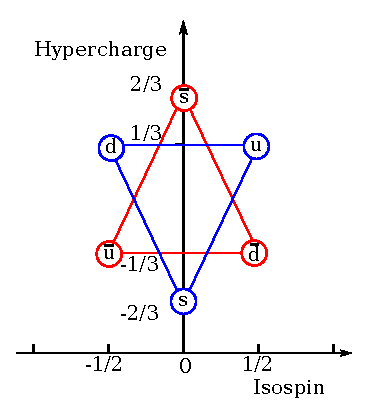
\includegraphics[width=0.3\textwidth]{theory/figures/threequarks}}\\
	\subfigure[]{
  	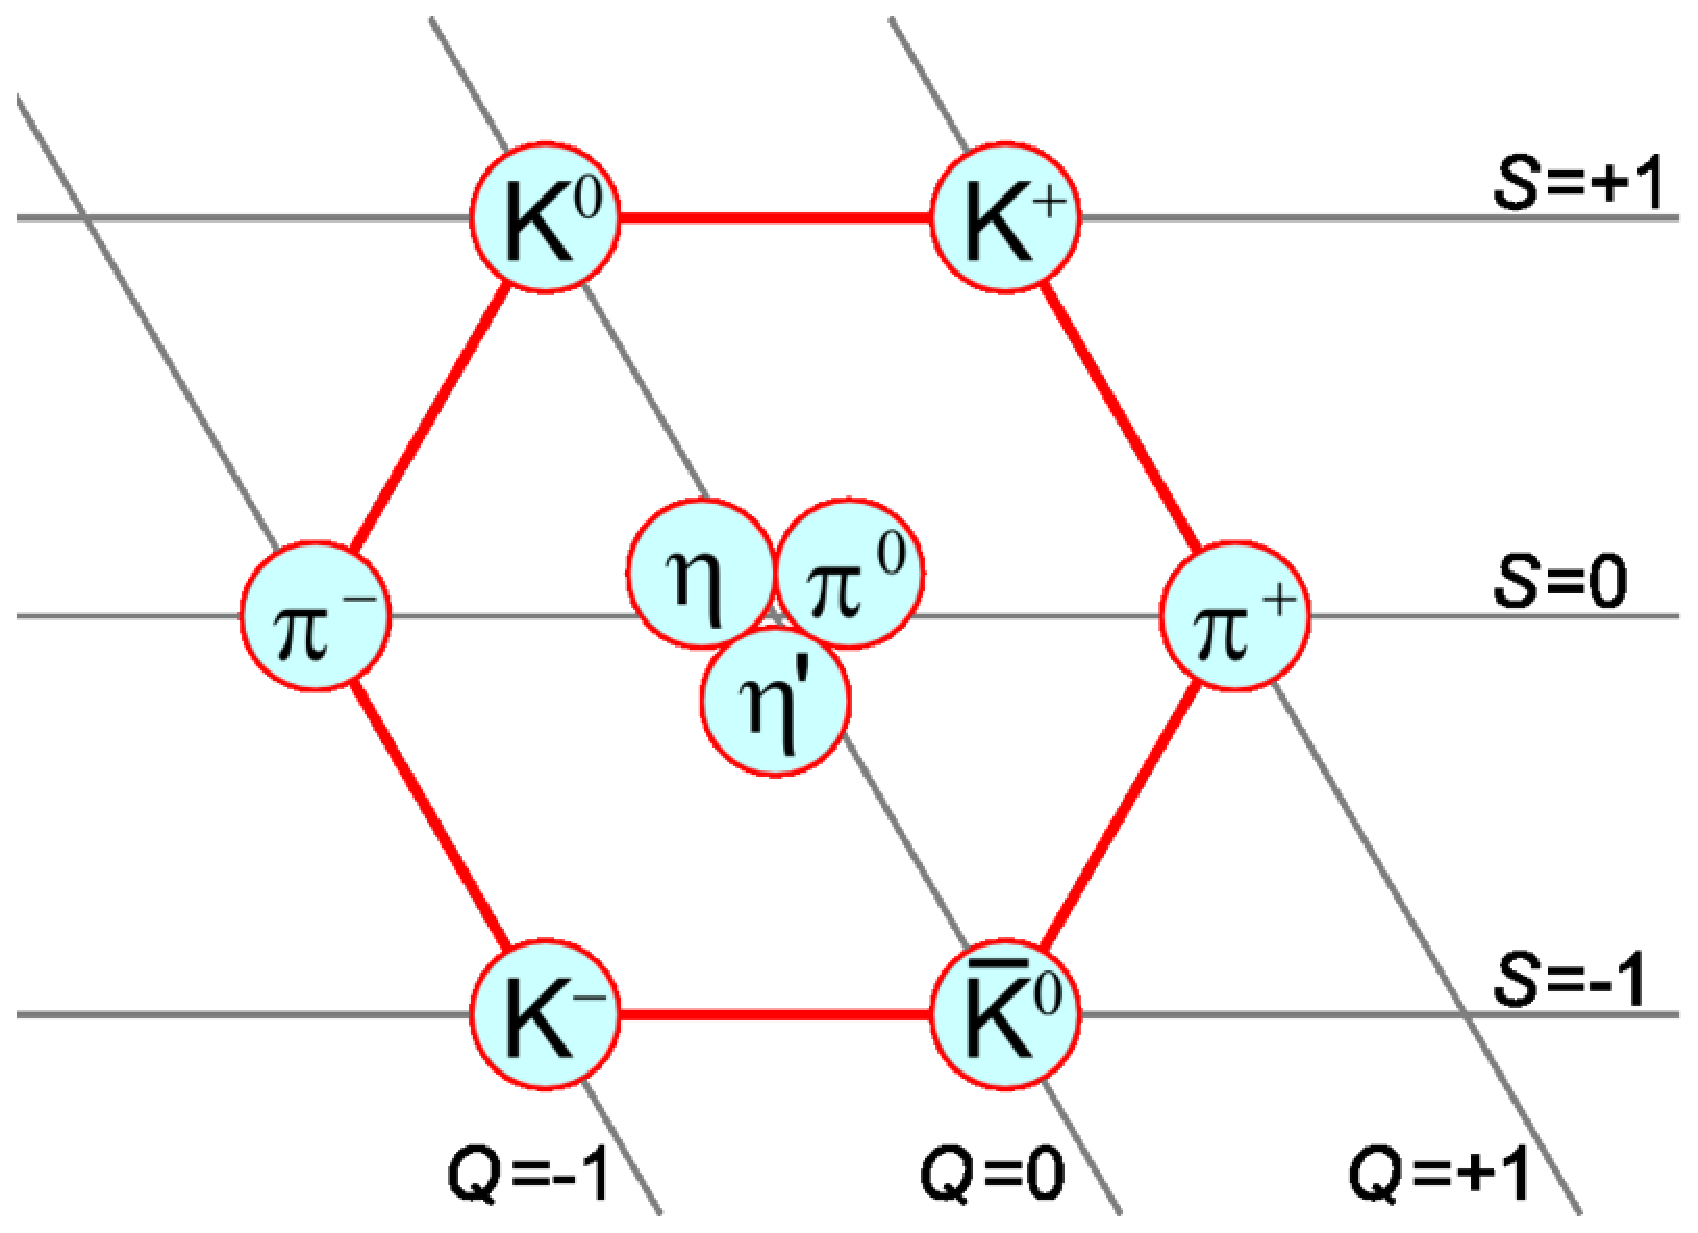
\includegraphics[width=0.37\textwidth]{theory/figures/mesons}}
	\subfigure[]{
  	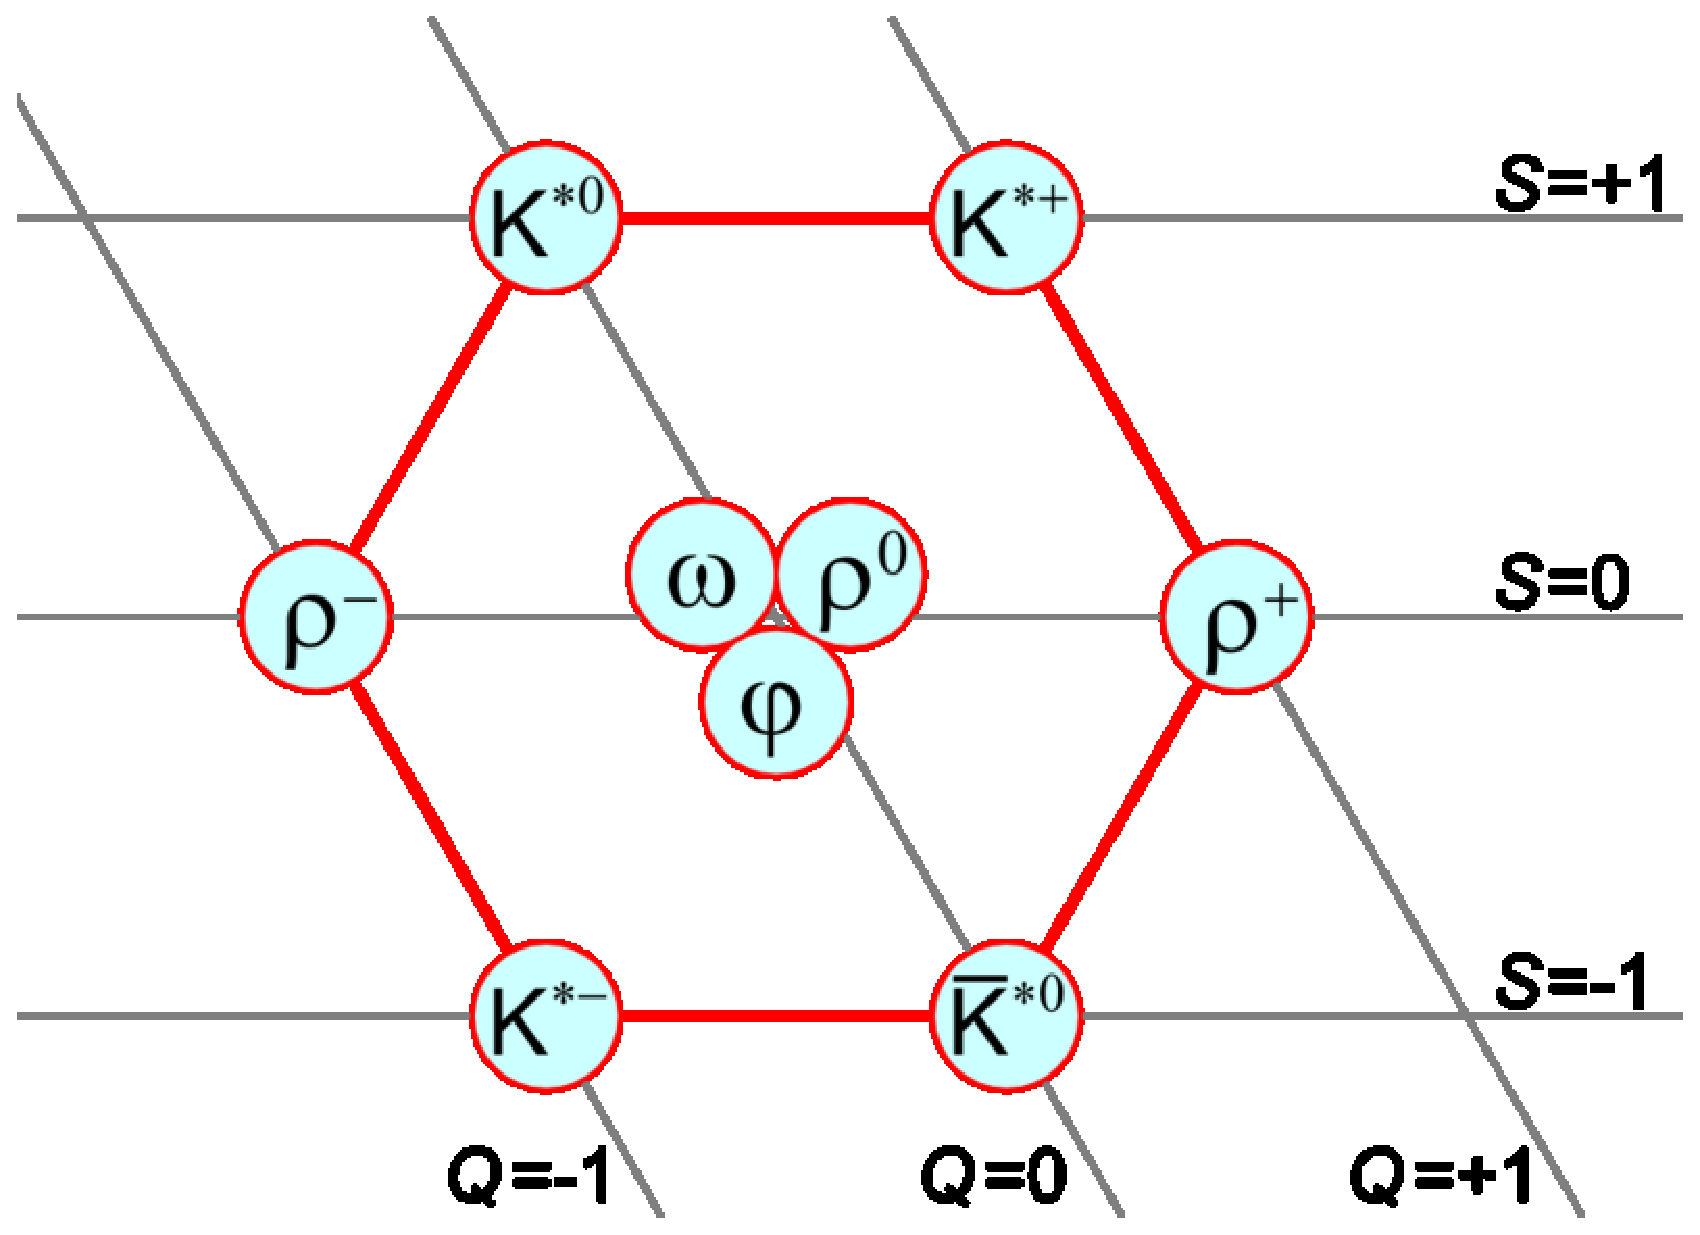
\includegraphics[width=0.37\textwidth]{theory/figures/mesons1}}
	\subfigure[]{
  	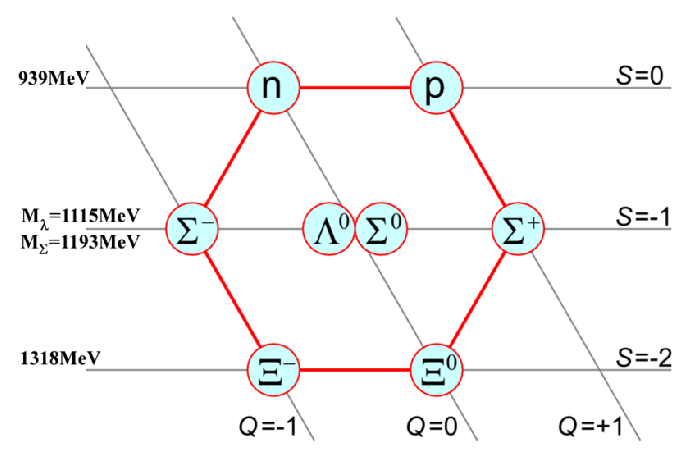
\includegraphics[width=0.4\textwidth]{theory/figures/Baryon_octet_w_mass}}
	\subfigure[]{
 	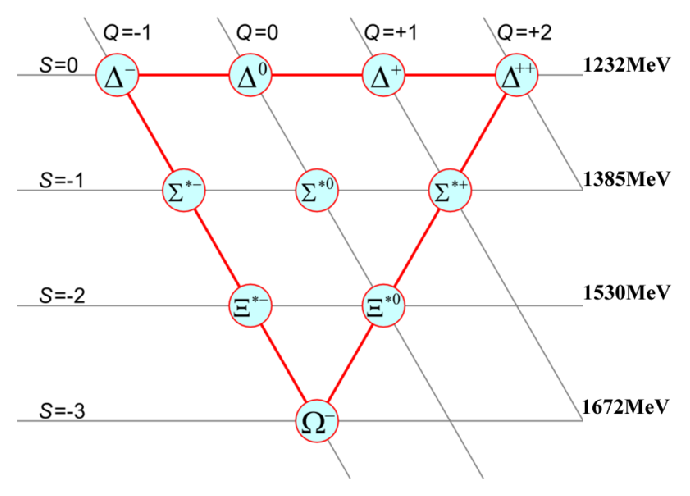
\includegraphics[width=0.4\textwidth]{theory/figures/Baryon_decuplet_w_mass}}
	\caption{Gell-Mann's \textit{Eightfold Way} (proposed also independently 
          by Yuval Ne'eman) identifies three fundamental components (a) 
          and classifies through their electric charge $q$ and strangeness $s$:
          a spin-0 meson octet (b), a spin-1 meson octet (c), 
          a spin-1/2 baryon octet (d) and a spin-3/2 baryon decuplet (e).
          It is now understood that this structure is a 
          consequence of flavour symmetry.\label{fig:eightfold}}
\end{center}\end{figure}

It was the beginning of the {\it quark model}, a theory that had to 
wait for multiple experimental evidence before being accepted,
nevertheless it successfully predicted a new particle, the strangeness $s$=-3 
particle $\Omega^{-}$ of the spin-3/2 baryon decuplet of Figure~\ref{fig:eightfold},
discovered in 1964 at Brookhaven~\cite{PhysRevLett.12.204}. 
Even when in 1968 deep inelastic experiments at the Stanford 
Linear Accelerator Center (SLAC) found out evidence for a 
substructure in protons~\cite{PhysRevLett.23.930,PhysRevLett.23.935}, physicists were reluctant to accept 
this point-like objects to be the quarks. Richard Feynman called 
them \textit{partons}, the term now used to identify quarks 
and antiquarks as well as gluons.

However, back then there was a tougher problem tormenting theoretical physicists. 
Quantum field theory was in fact apparently unsuitable for the description 
of the dynamics of particles interactions, since divergences appeared in the 
high energy domain. In 1954 Chen N. Yang and Robert Mills proposed a new gauge 
theory~\cite{PhysRev.96.191} based on the principle of {\it local gauge invariance},
i.e. the property of space-time regions of not being affected 
by a symmetry transformation performed 
locally in a different region. With the addition of a scalar 
field proposed by Peter Higgs, 
Fran\c{c}ois Englert and Robert 
Brout~\cite{PhysRevLett.13.321,PhysRevLett.13.508} and the implied 
modification of the vacuum structure, the Yang-Mills field 
became a very accurate description of the weak force interactions. 
Such unified model was consistently proposed, independently, in the 1960s 
by Abdus Salam, Sheldon Glashow and Steven 
Weinberg~\cite{Glashow1961579,PhysRevLett.19.1264}, 
but it suffered of a problem: 
as it was a perturbative theory, equations 
had to be expanded in a power series to be calculated but only the leading order 
term did not show ultraviolet divergences\footnote{Divergences in computations
are classified according to the energy scale at which they appear. Following
the Planck relation $E=h\nu$ and the relation between the wave lenght and
the frequency of radiation $\lambda\nu = c$, in natural units 
($\hbar=c=1$) energies of the order of 1~\tev\ 
or more lie in the ultraviolet (UV) range: $\lambda({\rm UV})\sim 10^{-9}$~m.
Divergencies appearing at the energy scale of 1~\gev\ or less are in the 
infrared (IR) range: $\lambda({\rm IR})\sim 10^{-6}$~m.}.

By the first years of the 1970s Gerard't Hooft demonstrated in his
PhD thesis under the supervision of  Martinus Veltman the
renormalization for the theory~\cite{tHooft1971173,Hooft1971167}, 
with the result that divergences could be 
cancelled and physical observables obtained with precisions higher than the 
leading order. 
The concept of \textit{renormalization group} was introduced and 
Yang-Mills theories were found to have a $\beta$-function (a function 
typical of gauge theories) generally negative. This was the discovery 
of \textit{asymptotic freedom}, a property that made Yang-Mills theory 
suitable also to describe strong interactions and that matched properly 
with the experimental effect named \textit{Bjorken scaling}\footnote{At 
SLAC it was observed during deep inelastic scattering experiments that 
strong interactions show a decrease of strenght at short distances (i.e. 
high momentum transfer) together with a scaling behaviour. A property is 
said to ``scale'' when it depends only by dimensionless kinematic quantities, 
such as a scattering angle or the ratio of the energy to a momentum transfer.}. 

At the same time, the three-quark model by Gell-Mann and Zweig was about to 
be expanded. In 1963 Nicola Cabibbo proposed the mixing of up, down and 
strange quark~\cite{PhysRevLett.10.531} 
in order to explain the non-conservation of quark flavour 
in weak interactions as $\Lambda \rightarrow p^{+}\pi^{-}$ with $\Delta S$=1 
and the empirical law $\Delta S = \Delta Q$ for strangeness changing processes. 
In 1970 Glashow, Iliopoulos and Maiani (GIM) predicted a fourth quark~\cite{PhysRevD.2.1285}, 
the charm, to account for the non-observation of Strangeness Changing Neutral 
Current (SCNC) processes. Thus, the quark mixing between the two families
of quarks ($u$, $d$) and ($c$, $s$) could be described with a $2\times 2$ 
matrix, parameterized by the Cabibbo angle $\theta_{C}$ and referred to as
 the Cabibbo-GIM matrix:
\begin{equation}\label{CabibboGIM}
V_{c} = {\setlength\arraycolsep{6pt}
\left( \begin{array}{cc}
\cos\theta_{C} & \sin\theta_{C}\\
-\sin\theta_{C}& \cos\theta_{C}
\end{array}
\right)} \quad .
\end{equation}
Furthermore, after the observation of events violating the Charge-Parity (CP) 
symmetry~\cite{PhysRevLett.13.286}, Makoto Kobayashi and 
Toshihide Maskawa supposed the 
existence of two more quarks, the bottom and the top, thus increasing 
the number of quark flavours to six~\cite{Kobayashi:1973fv}. 
This allowed the introduction in 
the extended $3\times 3$ mixing matrix (the Cabibbo Kobayashi Maskawa CKM matrix) 
of, besides three angles, a complex phase that is responsible of CP violation. 
All this conjectures found an important confirmation in November 1974, a date
later known as ``the November Revolution'' probably because it set the 
beginning of a real trust in the quark theory. 
Almost simultaneously at SLAC and at Brookhaven the charm quark was discovered 
in the bound state $c\bar c$, called $J$ meson by the Brookhaven team and 
$\psi$ by the SLAC one, so that in the end it was named $J/\psi$~\cite{PhysRevLett.33.1404,PhysRevLett.33.1406}. 
Not too much later, the bottom quark was observed in 1977 at 
Fermilab~\cite{PhysRevLett.39.252}, 
enhancing the belief in the top quark existence and in the six flavours theory.

The discovery of the tau lepton in 1975~\cite{PhysRevLett.35.1489} and of the 
$W$ and $Z$ bosons in 1983~\cite{Arnison1983103,Banner1983476,} finally set the scene for 
the Standard Model (SM) of particle physics. Table~\ref{tab:SM} 
shows the fundamental particles composing the SM: three generations of 
fermions, each of them having a corresponding 
antiparticle, the three forces (three Yang-Mills fields) with 
their vector bosons, and the Higgs boson whose field interaction with
particles results in the lagrangian mass terms. A great achievement of the SM was 
the unification of electromagnetic and weak theories in the Electroweak 
Theory by Salam, Glashow and Weinberg. In fact, since at a scale of about 
100~GeV the coupling constants converge, it is possible to describe them 
within the same mathematical model. Quantum ChromoDynamics (QCD) instead 
describes the strong interaction in terms of the color threefold charge 
and up to now is not known if also the strong coupling constant can become 
equal to the others at some high energy scale. However, a unified theory is 
strongly desired, as will be stressed in Section~\ref{sec:THquest}.
\begin{table}[htb]\centering\begin{tabular}{ccccc}\toprule
&\multicolumn{2}{c}{Leptons}&\multicolumn{2}{c}{Quarks} \\ 
& \multicolumn{2}{c}{spin 1/2}& \multicolumn{2}{c}{spin 1/2}\\
& $q=-1$ & $q=0$ &$q=2/3$ &$q=-1/3$ \\ \midrule
I & $e^{-}$ & $\nu_{e}$ & $u$ & $d$ \\
II & $\mu^{-}$ & $\nu_{\mu}$ & $c$ & $s$ \\
III & $\tau^{-}$ & $\nu_{\tau}$ & $t$ & $b$ \\\bottomrule\toprule
Force & Elm &\multicolumn{2}{c}{Weak}& Strong\\\midrule
Carrier boson & $\gamma$ & $W^{\pm}$ &$Z$ & $g$\\
spin & 1 & 1 &  1 & 1 \\
$q$ & 0 & $\pm$1 & 0 & 0\\\bottomrule\toprule
 \multicolumn{2}{c}{Higgs boson $H$}& \multicolumn{3}{c}{$q=0$, spin=0} \\
\bottomrule
\end{tabular}\caption{Elementary particles and forces of the SM.}\label{tab:SM} \end{table}

Even if the SM was somehow born to be merely a stepping stone, 
it consolidated through years, standing all experimental tests 
sometimes with a precision greater than 0.1\%. Experiments carried 
out at the Large Electron-Positron (LEP) collider at CERN, 
thanks to the clean signals given by $e^{+}e^{-}$ collision events, 
allowed to obtain very high precision measurements of the SM parameters
(see Figure~\ref{fig:smparam} for a summary of the measurements, with
their errors, of the free parameters of the SM).
\begin{figure}[htb]\begin{center}
	\subfigure{
  	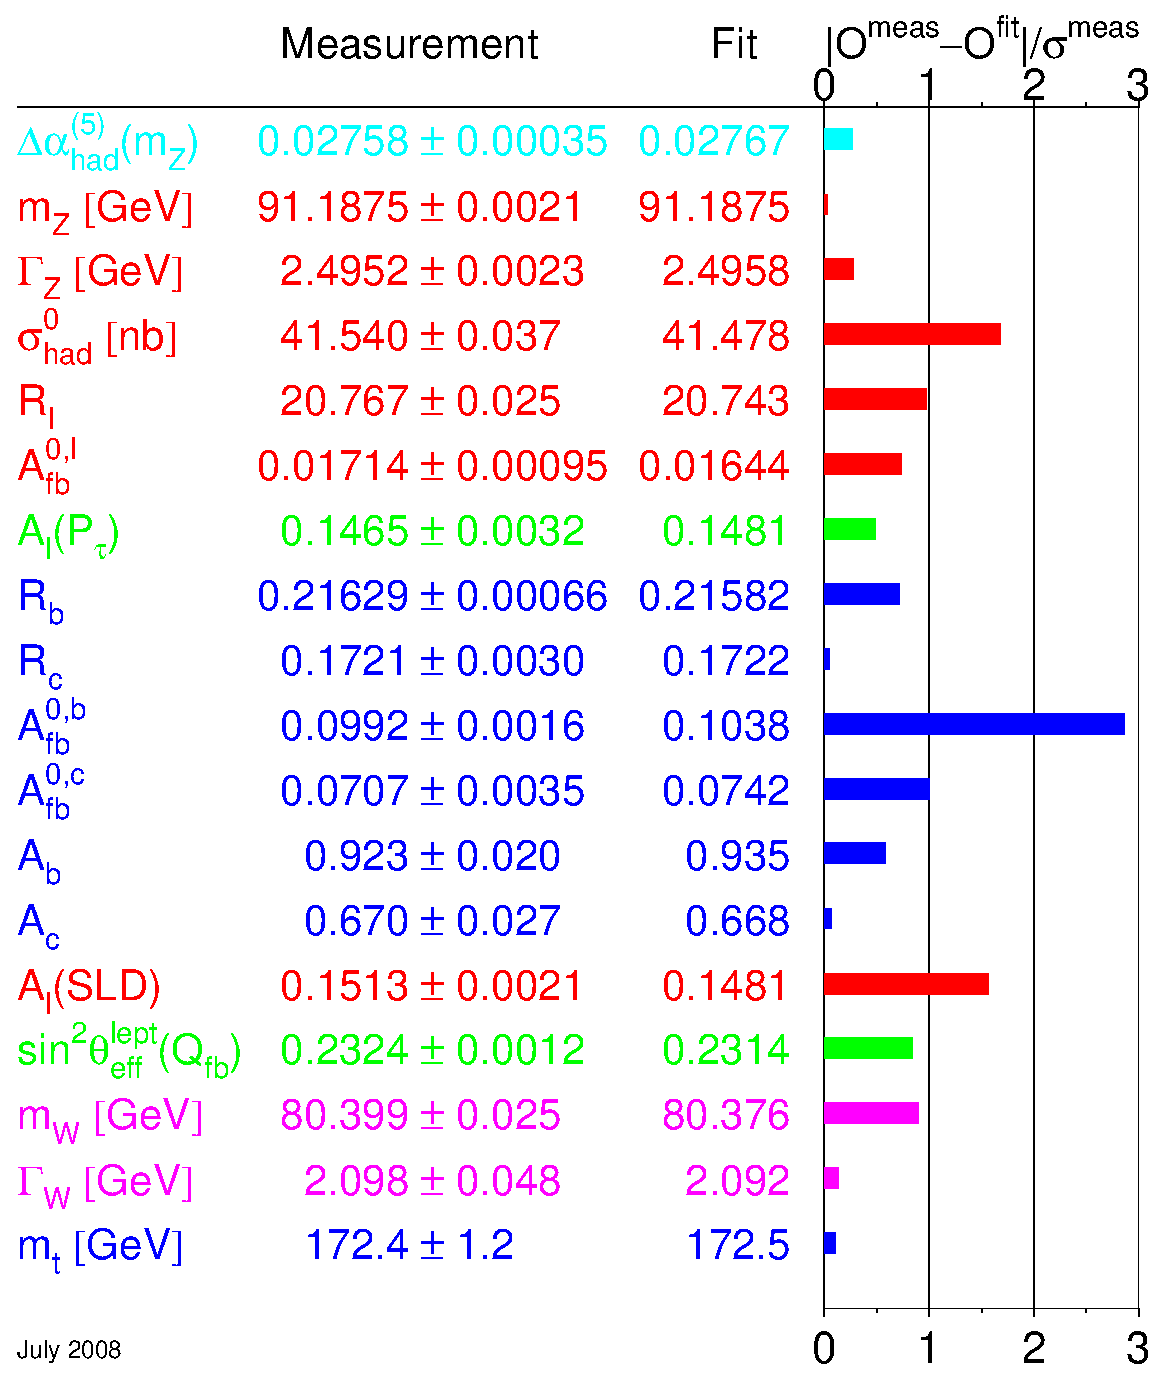
\includegraphics[width=0.4\textwidth]{theory/figures/fitSM}}%cernlep5_5-04}}
	\caption{Measured free parameters of the SM with the corresponding
          precision and the result of the consistency fit~\cite{Renton}.\label{fig:smparam}}
%\url{http://cerncourier.com/cws/article/cern/29076}}
\end{center}\end{figure}
 
In particular experiments ALEPH, DELPHI, L3 and OPAL performed the measurements 
of the $Z$ boson mass with a precision of 0.0023\% that made it one of the most 
precisely known quantities within the SM. %AAAAAAAAAAAAAAAAA \footnote{Note that the masses of the $W$ and $Z$ bosons are not predicted by the theory, but their ratio is (see Section~\ref{sec:ewlagr}).}. 
Furthermore, measurements of its total 
decay width and of its partial decay widths for all processes with a 
visible final state (i.e. different from $\nu\bar\nu$) allowed to set 
the number of light neutrino flavours to three, confirming the three-generation 
SM and excluding the possibility for a fourth family of leptons with masses
 lower than half of $m_Z$.

The penultimate discovery inside the SM has been the observation of the 
top quark in 1995 at the Fermilab's experiments CDF and 
D0~\cite{PhysRevLett.74.2626,PhysRevLett.74.2422}. 
The mass of the top quark resulted consistent with the predicted 
constraints, thus confirming again the SM as an accurate framework. 
At that point, and for almost 20 years, the last missing piece whose
absence could invalidate all the previous beautiful corroborations, was
the observation of a Higgs boson with a light mass for  self-consistency 
of the overall fit of data. When the LEP physics program was terminated,
direct searches gave, at 95\% CL, a lower limit of 114~\gev\ and an upper 
limit of 144~\gev\ on the mass of the Higgs boson~\cite{Renton}.

Then LEP was dismantled, the LHC was built, and in 2012 
the ATLAS and CMS experiments
observed a new $\sim$125~\gev\ mass boson~\cite{2012gk,Chatrchyan201230}
with the same spin-parity as the one expected from a Standard Model
Higgs boson. A precise {\it identikit} of this new particles, necessary
in order to say the final word about its nature (is it a Higgs boson?
Is it the Standard Model Higgs boson? Is it a ``new physics'' Higgs boson?),
is expected to come within the next decades of activity of the LHC and its
experiments.


\subsection{Building the Standard Model}\label{sec:THsm}

The Standard Model (SM) is a gauge theory invariant under the symmetry 
transformation $SU(3)_{C} \otimes SU(2)_{L} \otimes U(1)_{Y}$. The
three terms of the product of groups are the matrix representations
of the fundamental symmetries acting on the forces of Nature ({\it quantum fields})
governing the interactions of particles: 
$SU(3)_{C}$ is the {\it color} unbroken 
symmetry %containing the color triplets %, described by Quantum ChromoDynamics (QCD) 
 acting on the gluon field $G_a$; 
$SU(2)_{L} \otimes U(1)_{Y}$ is the unified {\it electroweak} broken 
symmetry, %described by Quantum ElectroDynamics (QED), 
with the weak symmetry $SU(2)_{L}$
%containing the left-handed weak isospin doublets 
acting on the vector boson fields $W_{1,2,3}$ and on the scalar Higgs field $\phi$,
and the electromagnetic symmetry $U(1)_{Y}$ %containing the right-handed isospin singlets.
acting on the vector boson field $B$ and on the scalar Higgs field $\phi$.

The quantum number $C$, the color charge, is carried only by
quarks, antiquarks and gluons 
in three different values labelled ``red'', ``gree'', ``blue''.
The quantum number $I$, the weak isospin, differentiates between left-handed
($I=1/2$) and right-handed ($I=0$) fermions, with the latter not undergoing weak interactions.
 %The quantum number $L$, the flavor charge, is carried by fermions as
 %{\it lepton number} for leptons and as {\it baryon number} for quarks.
The quantum number $Y$, the hypercharge, is defined as $Y=2(Q-I_3)$, 
where $Q$ is the electric charge and $I_3$ the third componend of the isospin,
which is $I_3=+1/2$ for up-type quarks and negatively charged leptons, and
 $I_3=-1/2$ for down-type quarks and neutrinos (and {\it vice-versa} for the antiparticles).

%These quantum numbers are the generators for the

Gravity is not (yet) included in the model, and even though
this is a flaw of the SM that is desirable to be fixed in a 
Grand Unified Theory (GUT), its action on particles is of many order
of magnitudes lower than the others' and is, therefore, negligible at the
fundamental components scale.


\subsubsection{Building the electroweak lagrangian}\label{sec:ewlagr}

The Lagrangian of the SM is built by {\it gauging} the symmetries in 
order to obtain invariance under those transformations.
Fermions are spin-1/2 particles that can be represented as spinors.
Using $\psi_{L}$ and 
$\psi_{R}$ to denote the left-handed and right-handed fermion fields 
respectively, 
the bare electroweak Lagrangian of the SM (considering 
for simplicity only leptons) is made of two terms:
\begin{equation}\label{eq:bareLagSM}
\mathcal{L}_{0} = \mathcal{L}_{lept}+ \mathcal{L}_{gauge}
\end{equation}
that are 
\begin{align}
&\left \{ \begin{array}{cl}
\mathcal{L}_{lept} &=\;\;  \bar\psi_{L}i\slashed{D}_{L}\psi_{L} + \bar\psi_{R}i\slashed{D}_{R}\psi_{R}\\
D_{L}^{\mu} &=\;\;  \partial^{\mu} + ig\dfrac{\bar{\sigma}\cdot\bar{W}^{\mu}}{2} + i\dfrac{g'}{2}Y_{L}B^{\mu}\\
D_{R}^{\mu} &=\;\;  \partial^{\mu} + i\dfrac{g'}{2}Y_{R}B^{\mu}
\end{array} \right. ,\label{eq:lagLep} \\
&\left \{ \begin{array}{cl}
\mathcal{L}_{gauge}  &=\;\;  -\frac{1}{4}W_{\mu\nu}^{l}W^{\mu\nu\, l}  -\frac{1}{4}B_{\mu\nu}B^{\mu\nu}\\
B_{\mu\nu} &=\;\;  \partial_{\mu}B_{\nu} - \partial_{\nu}B_{\mu}\\
W_{\mu\nu}^{l} &=\;\;  \partial_{\mu}W_{\nu}^{l} - \partial_{\nu}W_{\mu}^{l} - g\varepsilon^{jkl}W_{\mu}^{j}W_{\nu}^{k}
\end{array} \right. .\label{eq:lagGauge}
\end{align}
The gauge invariance is obtained through the definition of the
covariant derivatives $\slashed{D} = \gamma_{\mu}D^{\mu}$, 
which are different for the left- and
right-handed components of the field.
The chirality of the electroweak interactions does not find 
a theoretical motivation, but $SU(2)_{L} \otimes U(1)_{Y}$ transformations 
do make distinction between left and right helicity of the spinors.
Introducing the Weyl representation of the $\gamma$ matrices
\begin{equation}
\gamma^{0} = \left(\begin{array}{cc} 0 & 1 \\ 1 & 0 \\ \end{array}\right), \quad
\gamma^{i} = \left(\begin{array}{cc} 0 & \sigma^{i} \\ -\sigma^{i} & 0 \\ \end{array}\right) \quad \textnormal{and} \quad
\gamma^{5} = \left(\begin{array}{cc} -1 & 0 \\ 0 & 1 \\ \end{array}\right) \quad ,
\end{equation}
where $\sigma_{i}$ are the Pauli matrices, the left- and right-handed spinors transform as:
\begin{align}
&\left \{ \begin{array}{ll}
\psi_{L} = \frac{1}{2}(1 - \gamma_{5})\phi &\rightarrow \; \psi_{L}' = e^{iY\beta(x) + i\bar{\sigma}\bar{\alpha}(x)}\psi_{L} \\
\psi_{R} = \frac{1}{2}(1 + \gamma_{5})\phi &\rightarrow \; \psi_{R}' = e^{iY\beta(x)}\psi_{R}
\end{array} \right. .
\label{eq:chiral}
\end{align}

Equation~\ref{eq:lagLep} is the ``free matter'' Lagrangian 
describing the transformation under the symmetry $SU(2)_{L}$ of weak isospin
with coupling constant $g$, three boson fields $W^{l}_{\mu\nu}$ and
their weak generators $\bar{\sigma}$\footnote{These are the Pauli matrices: 
$$
\sigma_{1} = \left(\begin{array}{cc} 0 & 1 \\ 1 & 0 \\ \end{array}\right), \quad
\sigma_{2} = \left(\begin{array}{cc} 0 & -i \\ i & 0 \\ \end{array}\right), \quad
\sigma_{3} = \left(\begin{array}{cc} 1 & 0 \\ 0 & -1 \\ \end{array}\right).
$$}, and under the symmetry
$U(1)_{Y}$ of hypercharge with coupling constant $g'/2$,
the boson field $B_{\mu\nu}$ and its hypercharge generator $Y$.
Equation~\ref{eq:lagGauge} is the Lagrangian for the vector bosons 
dynamics with self-couplings, including trilinear and quadrilinear terms. 



The Lagrangian \ref{eq:bareLagSM} is invariant under group 
$SU(2)_{L} \otimes U(1)_{Y}$ transformation, but has the 
problem of leaving fermions massless. Thus a scalar 
Lagrangian with a quartic auto-interaction is introduced:
\begin{equation}\label{eq:lagScalar}
\left \{ \begin{array}{cl}
\mathcal{L}_{\phi} &=\;\;  (D_{\phi}^{\mu} \phi)^{\dag}(D_{\phi\,\mu} \phi) - V(\phi^{\dag}\phi)\\
V &=\;\; \mu^{2}\phi^{\dag}\phi + \lambda(\phi^{\dag}\phi)^{2}\\
D_{\phi}^{\mu} &=\;\; \partial^{\mu} + ig\dfrac{\bar{\sigma}\cdot\bar{W}^{\mu}}{2} + i\dfrac{g'}{2}Y_{\phi}B^{\mu}
\end{array}\right. ,
\end{equation}
where $\phi$ is an Higgs doublet, accounting for four 
degrees of freedom needed to give mass to three vector
bosons (the neutral $Z$ boson and the two $W^{\pm}$ bosons)
and to a scalar Higgs boson:
\begin{equation}\label{eq:higgsDoub}
\phi = \begin{pmatrix} \varphi^{+}\\\varphi^{0}
\end{pmatrix} =
\dfrac{1}{\sqrt{2}} 
\begin{pmatrix} \varphi_{1}+i\varphi_{2}\\ \varphi_{3}+i\varphi_{4}\end{pmatrix}.
\end{equation}

%Three terms, $\varphi^{+}$, $\varphi^{-}$ and $(\varphi^{0}-\bar\varphi^{0})/\sqrt{2}$, give mass to the three massive vector bosons $W^{\pm}$ and $Z$, leaving a massive Higgs scalar boson $(\varphi^{0}+\bar\varphi^{0})/\sqrt{2}$. 
The potential $V(\phi)$ depends on two parameters, $\mu^2$ and $\lambda$. 
The case $\lambda<0$ is unphysical, leading to no stable minima. For 
$\lambda>0$, two cases arise: $\mu^2>0$ and $\mu^2<0$. In the first case
(see Figure~\ref{fig:higgs1}) there is a single solution to the minimization
which corresponds to $|\phi|=0$ and gives as vacuum expectation value
$\bra{0}\phi \ket{0} = 0$. In the second case (see Figure~\ref{fig:higgs2}) 
the potential has a non-vanishing vacuum expectation value 
$\bra{0}\phi \ket{0} = v$ and %the symmetry is spontaneously broken, the minimum not being unique anymore.
the minimum is not unique anymore. The fundamental vacuum 
state is no more invariant under $SU(2)_{L} \otimes U(1)_{Y}$, 
meaning that these two symmetries are now 
broken\footnote{Instead, the symmetry $U(1)_{elm} \subset SU(2)_{L} \otimes U(1)_{Y}$ 
is not broken. This means that vacuum is electrically uncharged while 
it has isospin and hypercharge charges.}: 
this is the Spontaneous Symmetry Breaking (SSB) mechanism. 
The vacuum state is chosen as:
\begin{figure}[htb]\begin{center}
	\subfigure[]{\label{fig:higgs1}
  	\includegraphics[width=0.45\textwidth]{theory/figures/higgs1.eps}}
	\subfigure[]{\label{fig:higgs2}
  	\includegraphics[width=0.45\textwidth]{theory/figures/higgs2.eps}}
	\caption{Vacuum pontential for $\lambda>0$ and (a) $\mu^2>0$ or
          (b) $\mu^2<0$, with the typical shape of a mexican hat~\cite{Michael:1569839}.}
\end{center}\end{figure}

\begin{equation}\label{eq:vacuum}
\phi_{0} = \begin{pmatrix} 0 \\ v/\sqrt{2}
\end{pmatrix}
\end{equation}
where $v = \sqrt{-\mu^{2}/\lambda}$ is 
the vacuum expectation value. Finally, since
only the vector bosons got their mass up to now,
the only thing left to do is to introduce 
the scalar-fermion interaction in order to give
mass to the fermions. This is done defining:
\begin{equation}\label{eq:lagYukawa}
\mathcal{L}_{Yukawa} = -G_{lept}\big[\bar\psi_{R}(\phi^{\dag}\psi_{L}) + (\bar\psi_{L}\phi)\psi_{R}\big] .
\end{equation}Thus the complete electroweak Lagrangian of the SM, that can be generalized also to quarks (see Table \ref{tab:isospin}), is\begin{equation}\label{eq:lagSM}
\mathcal{L}= \mathcal{L}_{lept} +\mathcal{L}_{gauge} +\mathcal{L}_{\phi} +\mathcal{L}_{Yukawa}.
\end{equation}

\begin{table}[htb]\centering\begin{tabular}{cccc}\toprule
\multicolumn{4}{c}{Weak isospin left-handed doublets \bfseries $\psi_{L}$} \\ \midrule \\ 
$\begin{pmatrix} \nu_{e_{L}} \\ e_{L} \end{pmatrix}$ & $\begin{pmatrix} \nu_{\mu_{L}} \\ \mu_{L} \end{pmatrix}$ &$\begin{pmatrix} \nu_{\tau_{L}} \\ \tau_{L} \end{pmatrix}$ & \bfseries Leptons \\ \\ 
$\begin{pmatrix} u_{L} \\ d'_{L} \end{pmatrix}$ & $\begin{pmatrix} c_{L} \\ s'_{L} \end{pmatrix}$ &$\begin{pmatrix} t_{L} \\ b'_{L} \end{pmatrix}$ & \bfseries Quarks \\
 \\ \bottomrule\\ \toprule
\multicolumn{4}{c}{Weak isospin right-handed singlets \bfseries $\psi_{R}$} \\ \midrule \\ 
$ e_{R} $ & $ \mu_{R}$ &$\tau_{R}$ & \bfseries Leptons \\ \\ 
$u_{R}$ , $d'_{R} $ & $c_{R}$ , $s'_{R} $ &$ t_{R}$ , $b'_{R}$ & \bfseries Quarks \\
 \\ \bottomrule
\end{tabular}\caption{Weak isospin multiplets. $q'$ refers to the flavour eigenstate that correspond to the mass eigenstate transformed with the CKM matrix.}\label{tab:isospin} \end{table}

An important consequence of the introduction of the scalar Higgs 
field and the consequent spontaneous symmetry breaking
is the mixing of the vector bosons $B_{\mu}$ and $W^{1,2,3}_{\mu}$ 
to give the photon $A_{\mu}$, the two $W^{\pm}_{\mu}$ and 
the $Z_{\mu}$ bosons:
%\begin{equation}\label{eq:AZ}
%\left \{ \begin{array}{ll}
%A^{\mu} = \cos\theta_{W}B^{\mu} + \sin\theta_{W}W_{3}^{\mu}\\
%Z^{\mu} = -\sin\theta_{W}B^{\mu} + \cos\theta_{W}W_{3}^{\mu}\end{array}\right. ,
%\end{equation}
\begin{align}
  W_{\mu}^{\pm} & = \frac{1}{\sqrt{2}}\left(W_{\mu}^{1}\mp i W_{\mu}^{2}\right), \label{eq:Wpm} \\
  \left(
  \begin{array}{c}
  A_{\mu} \\ Z_{\mu}
  \end{array}
  \right)
  & =
  \left(
  \begin{array}{cc}
  \cos\theta_{W} & \sin\theta_{W} \\
  -\sin\theta_{W} & \cos\theta_{W}
  \end{array}
  \right)
  \left(
  \begin{array}{c}
  B_{\mu} \\ W_{\mu}^{3}
  \end{array}
  \right) , \label{eq:AZ}
\end{align}
where the Weinberg angle $\theta_{W}$ is defined through\begin{equation}\label{eq:weinb}
\left \{ \begin{array}{ll}
\dfrac{g}{\sqrt{(g')^{2}+g^{2}}} = \cos\theta_{W} \\
\dfrac{g'}{\sqrt{(g')^{2}+g^{2}}} = \sin\theta_{W} \end{array}\right. .
\end{equation} Masses acquired through the Higgs mechanism are listed in Table \ref{tab:mass}.


\begin{table}[htb]\centering
\begin{tabular}{cccc}\toprule
\multicolumn{4}{c}{Force Carriers} \\ \midrule
$\gamma $ &$W^{\pm}$ &$Z$ &$g$ \\
$0$ & $\sqrt{\dfrac{g^{2}v^{2}}{4}} $& $\sqrt{\dfrac{(g^{2}+g'^{2})v^{2}}{4}} $&  $0$ \\
$0$ & $80.4$ & $91.2$ & $0$ \\\bottomrule\\
\end{tabular}
\begin{tabular}{cccccccccc}\toprule
\multicolumn{10}{c}{Leptons and Quarks} \\ \midrule
$e$ & $\mu$ &$\tau$ &$\nu$ & $u$ & $d$ & $c$ & $s$ &$ t$ & $b$ \\
\multicolumn{10}{c}{$\dfrac{v}{\sqrt{2}}g_{f}$} \\
$0.511\cdot10^{-3} $ & 0.105 & 1.777 & $\sim0$ & 0.0024 & 0.0048 & 1.27 & 0.104 & 171.2 & 4.2 \\\bottomrule
\end{tabular}\caption{Particle Masses in GeV.}\label{tab:mass} \end{table}


\subsubsection{Adding the strong interaction}\label{sec:qcdlagr}

Adding the color transformations $SU(3)_{C}$, the Standard Model is
finally described by the symmetry group 
$SU(2)_{L}\otimes U(1)_{Y}\otimes SU(3)_{C}$.
In the same way electromagnetic interactions are 
described by Quantum ElectroDynamics (QED), 
strong interactions are described by Quantum ChromoDynamics (QCD~\cite{Ecker}).
However, while the photon does not carry electric charge,
the gluon does carry color charge (in particular it exists in
eight states, being a color octet) and can, therefore, self-interact.

The QCD lagrangian only involves quarks and gluons, and reads:
\begin{equation}
\left \{ \begin{array}{cl}
\mathcal{L}_{QCD} &=\;\; \sum\limits_{f=1}^{6}\bar{q}(i\gamma^\mu D_\mu - m_q)q 
                    -\frac{1}{4}F^{\mu\nu}_{a}F^{a}_{\mu\nu}\\
 D_\mu &=\;\; \partial_\mu + ig_sG_\mu^a T^a\\
  F^{a}_{\mu\nu} &=\;\;  \partial_\mu G_\nu^a - \partial_\nu G_\mu^a - 
                    gf^{a}_{\ bc}G^b_\mu G^c_\nu
\end{array} \right.
\end{equation}
where $q$ is the quark field and $m_q$ is the quark mass, summed over 
the six types of quarks, and $a$ runs over the eight degrees of 
freedom of the gluon field, $T^a$ being the generators
of the $SU(3)_C$ group. The field tensor $F^{a}_{\mu\nu}$ 
is derived from the gluon field $G_\mu^a$ and 
its third term describes the gluon self-interaction, with
$f^a_{\ bc}$ being the structure constants. 
%non-abelian nature  of the QCD, and it describes the
The strong coupling constant $\alpha_s$ is defined
as  $\alpha_s=g/4\pi$ and its values, large at
low energies (i.e. large distances), and small at high 
energies (i.e. short distances), determine the 
peculiar property called {\it asymptotic freedom} which
explains the confinement of the quarks inside the hadrons
(see Figure~\ref{fig:alpha_s}). Indeed, at
small distances $\alpha_s$ is so low that
the strong interaction can be treated perturbatively
and quarks and gluons described as free particles.
On the other hand, a quark cannot be found
isolated since at large distances the field strength
will increase enough to create new quarks 
from the vacuum and colorless hadrons will be formed.

\begin{figure}[tbph]
\begin{center}
\subfigure{
  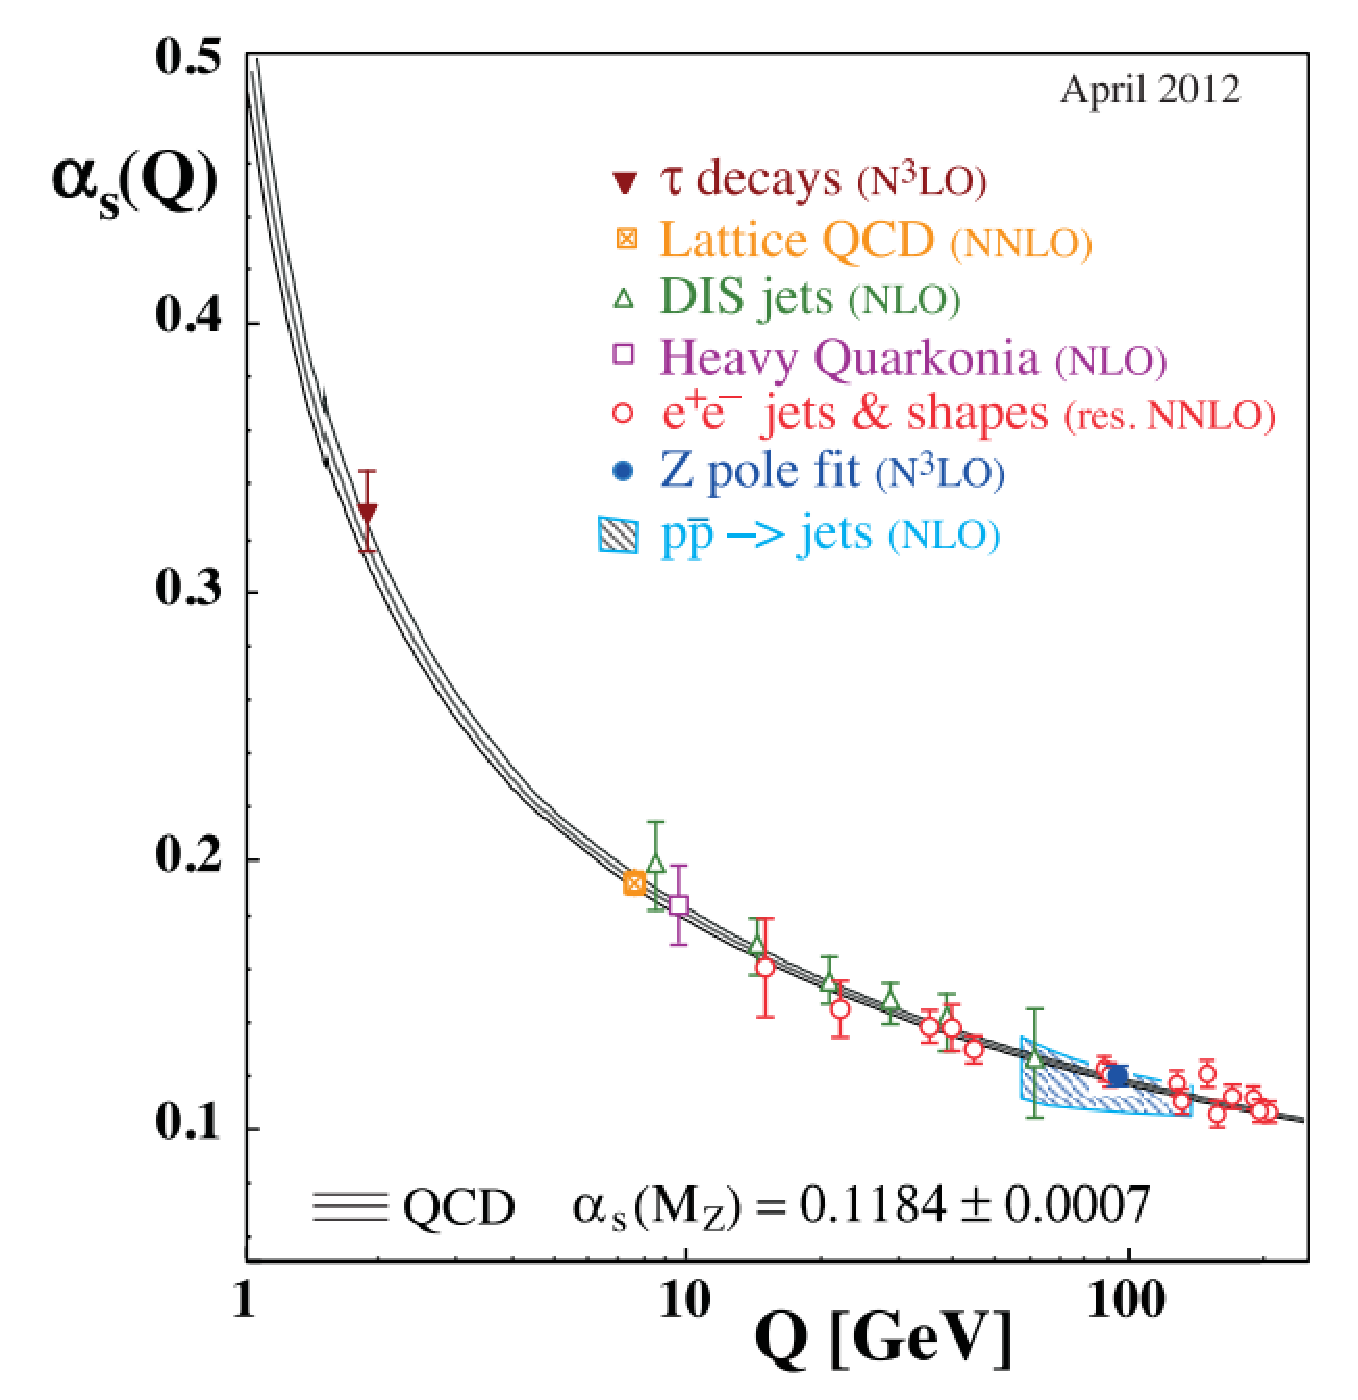
\includegraphics[width=0.5\textwidth]{theory/figures/asq-2012.eps}
}
\caption{Running of the strong coupling $\alpha_s$ with the energy scale $Q$,
proven from different measurements~\cite{alpha_s}.}
\label{fig:alpha_s}
\end{center}
\end{figure}

As an example of how quarks behave in hadrons,
protons are composed of two {\it valence} up quarks
and one {\it valence} down quark. The quarks continuosly
exchange gluons, which create in turn quark-antiquark pairs,
resulting in what is referred to as a ``sea'' 
of quarks and gluons. 
%randomly created and annihilated in vacuum fluctuations. 
As the sum of the rest masses of the valence quarks contributes 
only to about 1\% of the total nucleon
mass, what accounts for the missing 99\% is the
binding energy of gluons and sea quarks.
Further details on QCD will be given in Section~\ref{sec:MCphenomenology},
where the phenomenology of proton-proton collision
is discussed.



\section{Unanswered questions and new physics quests}\label{sec:THquest}

In the case the new boson discovered in July 2012 
really is a Standard Model Higgs boson, there would
be no more arguments to contradict the Standard Model
as an {\it effective theory}. Indeed many facts, both 
in theory and experiments, hints that the Standard Model,
despite is great success in describing the interaction
of fundamental particles, might be just an approximation
at low energy regimes of a more complete theory.

One of the principal objections to the Standard Model as 
``the final theory'' is the high number of arbitrary parameters 
of the theory. In fact, 19 parameters are needed to fit 
data from experimental observations. 
Three of them  are the couplings of the gauge groups 
$g_3, g, g'$ for the strong, electromagnetica and weak 
interactions respectively, also written as: 
\begin{equation}\label{eq:couplings}
\alpha_{s}=\dfrac{g_{3}^{2}}{4\pi} ,\quad 
\alpha_{elm} = \dfrac{e^{2}}{4\pi} =  \dfrac{g^{2}\sin^{2}\theta_{W}}{4\pi}, 
\quad \sin^{2}\theta_{W} = \dfrac{(g')^{2}}{g^{2}+(g')^{2}}.
\end{equation}
Then, 13 parameters are associated with the nine charged 
fermion masses and the four parameters of the CKM matrix 
(three quark-mixing angles and one phase), 
two are needed to describe the Spontaneous Symmetry Breaking mechanism, 
i.e. the Higgs vacuum expectation value $v$ and 
the quartic coupling constant $\lambda$, and the last one is the 
QCD $\theta$ parameter. Additionally, if neutrinos are massive 
(as it is almost certain from neutrino oscillation observations, 
see e.g. \cite{Langacker:817840}) there will be even more arbitrary 
parameters describing their masses and their mixing. 
Furthermore, massive neutrinos cannot exist in the Standard
Model, where only left-handed neutrinos are predicted and thus
no Dirac mass term can appear\footnote{A way out of this
problem postulates a new type of neutrinos, namely 
{\it Majorana neutrinos}, in contrast to {\it Dirac neutrinos}.}.


%If, based on these considerations,  one assumes that 
The arbitrariety of parameters, and in particular of the
fermion masses, introduces what goes under the name of
{\it naturalness problem}. A ``natural'' theory is
characterized by free parameters with values at, more or
less, the same order of magnitude. This does not happen in
the Standard Model, where the top quark, as an example,
has a mass $\sim 10^5$ larger than the up quark.
This issue further develops as follows. If the 
Standard Model is valid only up to  an energy scale 
$\Lambda$ (which, if it's the Planck scale, differs
from the electroweak scale by $\sim 10^{17}$!), 
then the scalar Higgs boson mass 
should encounter radiative corrections from 
vacuum polarization diagrams (like the one in Figure~\ref{topLoop}) 
of the order of $\Lambda$ giving to the mass the 
value: %~\cite{dawson-1997}:
\begin{equation}\label{eq:higgsMass}
M_{H}^{2} \sim M_{H_{0}}^{2} 
+ \dfrac{\lambda}{4\pi^{2}} \Lambda^{2} 
+ \delta M_{H}^{2}. \end{equation}
If the mass counterterm $\delta M_{H}^{2}$ does not 
cancel the quadratically divergent contribution and 
if the cutoff scale is chosen as the Planck scale, then
\begin{equation}
M_{H}^{2} \sim 10^{32},\end{equation} 
i.e. many orders of magnitude bigger than the experimentally 
measured value coherent with the Standard Model 
and with the unitarity constraint. This  
is the \textit{hierarchy problem}, and 
could be fixed within the Standard Model by 
choosing a fine-tuned mass counterterm, a 
solution considered not really elegant also 
because fine tuning will be required for every 
order in the perturbative expansion\footnote{This 
problem does not arise with loop corrections to 
fermion masses, which are protected by chiral 
symmetry, nor with boson masses,
which are protected by gauge invariance. It
is, actually, an issue of scalar particles
like the Higgs boson.}. %and that's the reason why fermion masses are said to be ``natural''.} 


\begin{figure}[htb]\begin{center}
%\includegraphics[width=.2\textwidth]{theory/figures/loop1}
\subfigure{ \def\svgwidth{0.25\textwidth}
\input{theory/figures/mod_loop1.eps_tex}}
\caption{The typical vacuum polarization diagram 
  for the Higgs is a top quark loop.}
\label{topLoop}\end{center}\end{figure}
%This argument looks the same of what made physicists pass from Fermi theory to Standard Model. In fact at that time the Fermi point like interactions were a good description of weak scattering processes of fermions $f+f\rightarrow f+f$, but the unitarity  predicted that at an energy $E_{crit} \sim 600$ GeV the theory would become inconsistent. Then it was found that new physics (the vector bosons of the Standard Model) was needed already from an energy scale about 100 GeV, maybe due to the small coupling constant of weak interaction. Now, the scattering process $W+W\rightarrow W+W$ has a scattering amplitude growing linearly to the self-coupling constant of the Higgs field $\lambda$. The formula for the critical energy is now related to the Higgs mass as \cite{Ho-Kim} $$\dfrac{E_{crit}}{v} = \exp\bigg(\dfrac{4\pi^{2}v^{2}}{3M_{H}^{2}}\bigg),$$ which for an higgs Higgs mass less than 150 GeV gives $E_{crit} \sim 10^{18}$, thus making the Higgs model valid up to that scale. However for an heavier Higgs with a mass about 700 GeV, such critical energy goes down to $10^{3}$ GeV.  It is to remark that in the electroweak interactions the Higgs contribution to radiative corrections is very low since is denoted by a logarithm function, thus giving low variations and not affecting the precision electroweak data. The meaning of this is, whatever the critical energy value will be, the Standard Model is an effective theory embedded in a more fundamental theory with $E_{crit}$ acting as a cutoff.

\begin{figure}[h!tb]\begin{center}
        \subfigure{ %\def\svgwidth{0.9\textwidth}
\input{theory/figures/mod_scales.eps_tex}}
	\caption{Typical length and energy scales
          of some of the fundamental parameters
          of the Universe.\label{fig:scales}}
\end{center}\end{figure}

Another disturbing feature of the Standard Model as it is 
is the lack of theoretical explanation for the generations 
of quarks and leptons to be exactly three, as suggested
(under certain assumptions) by precision measurements 
performed at LEP at the $Z$-pole ($\rts\sim 91$~\gev). 
From QCD comes the only constraint for quark generation
to be less that nine.

Cosmology and cosmological observations also challenge 
the Standard Model. The reason for baryon-antibaryon 
asymmetry is still not understood although we know 
that it is connected to  CP violation\footnote{The CP violating 
phase introduced in the CKM mechanism cannot, however, 
account for the total baryon-antibaryon asymmetry measured.}. 
Besides, astronomical observations~\cite{Ade:2013zuv} 
tell us that the energy density of the 
Universe is made only for a 4-5\% of ordinary baryonic 
matter, the other components being dark matter (20-25\%) 
and dark energy (70-76\%). Dark matter is non-baryonic 
matter that interacts only weakly and gravitationally and,
therefore, cannot be observed with telescopes but it
is revealed by its gravitational interaction with ordinary 
matter in space. 
It is now believed that Dark Matter is composed  of 
Weakly Interacting Massive Particles (WIMPs) whose 
masses range from a few GeV to a few TeV and  are 
not predicted within Standard Model. Dark energy instead is 
still more mysterious and maybe new physics will 
give some hints for its interpretation.

Another topic making the Standard Model likely to 
need improvements is the desire to go further in 
the unification of theories. Gravity is not 
implemented in the Standard Model, nor is available
a widely accepted quantum theory of gravity.
This is acceptable at the electroweak scale of 
few hundreds of GeV where the strength of gravity
is negligible, but its effect should become relevant 
going up to the Planck scale $\Lambda \sim 10^{19}$ GeV. 
Also, electroweak and strong forces forming the Standard 
Model gauge group $SU(2)_{L}\otimes U(1)_{Y}\otimes SU(3)_{C}$ 
are expected to unify at high energy since their coupling 
constants are running constants dependent on the energy 
scale (Figure~\ref{running}, $\alpha^{-1}_{i} = g^{2}_{i}/(4\pi)$). 
\begin{figure}[htb]\begin{center}
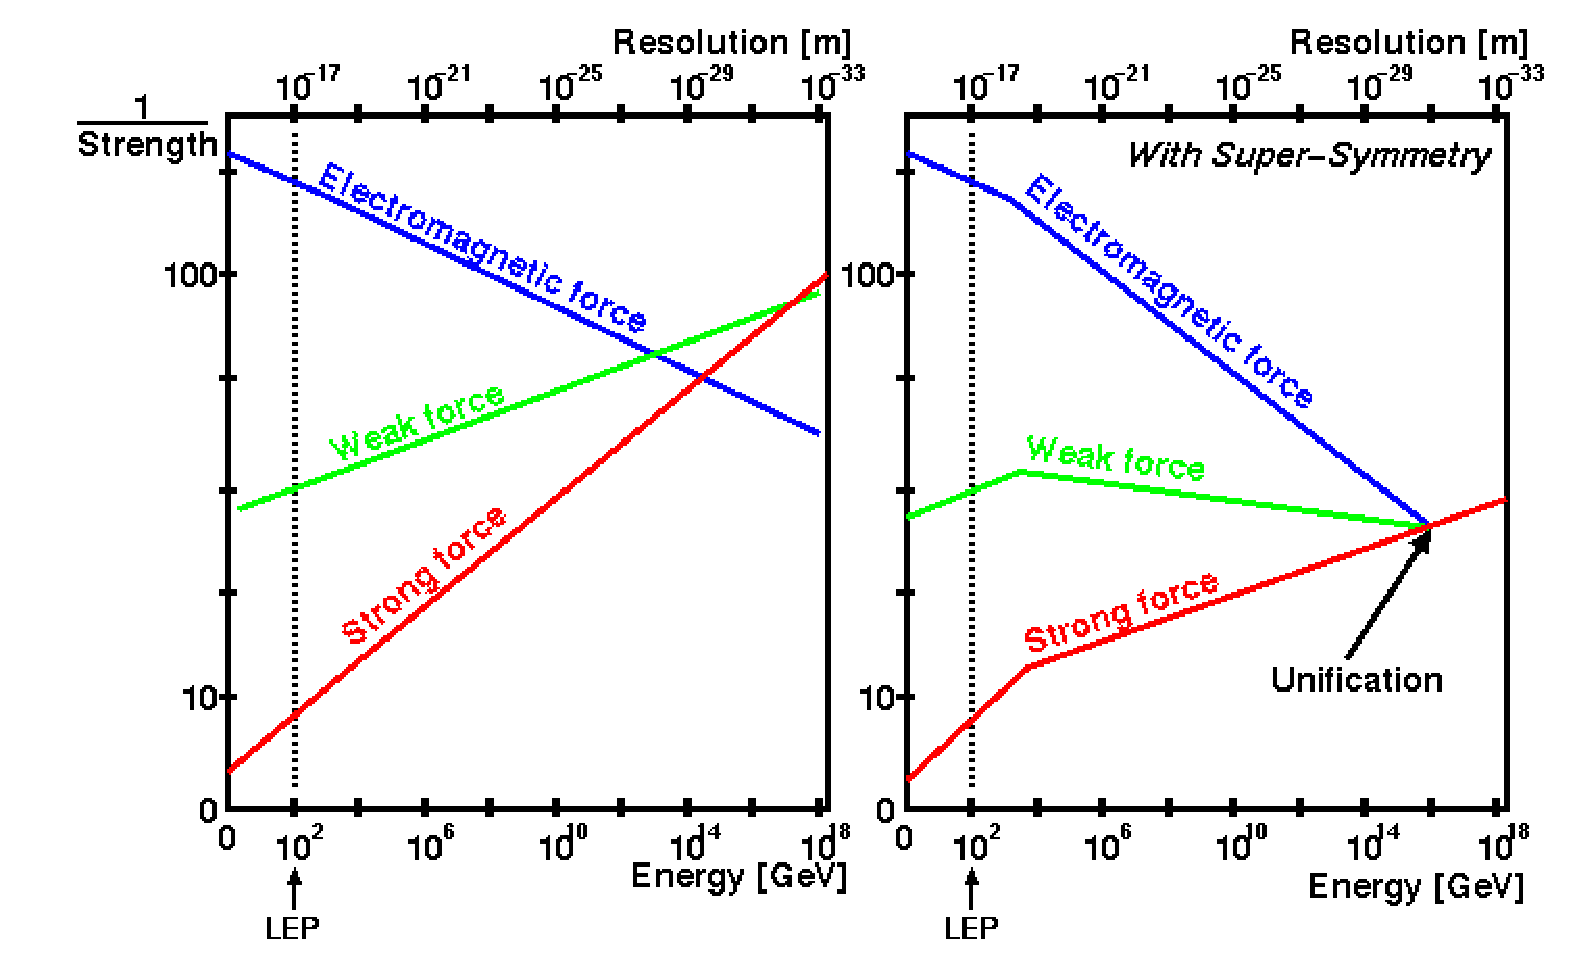
\includegraphics[width=.8\textwidth]{theory/figures/running_coupling}
\caption{Running coupling constants in the Standard Model (left) and 
in a hypothetical Supersymmetric Model (right, see Section~\ref{sec:susy}) 
as functions of the renormalization scale (picture from \url{http://scienceblogs.com},
original credits unknown). The energy scale explored at LEP is marked
on the two figures and corresponds to $10^2$~\gev. The LHC is able to
go just one order of magnitude further.}
\label{running}\end{center}\end{figure}

In the following some ``beyond-Standard Model'' theories
proposed to solve most of the issues illustrated
before are briefly illustrated.


\subsection{Supersymmetry}\label{sec:susy}

\subsection{Little Higgs}

\subsection{Extra-dimensions}





\section{Going beyond the SM with vector-like quarks}\label{sec:THvlq}

\cite{AguilarSaavedra:2009es,Martin:2009bg}

\subsection{Production}\label{sec:vlqprod}


\subsection{Decay}\label{sec:vlqdecay}






\clearpage{\pagestyle{empty}\cleardoublepage}
\clearpage{\pagestyle{empty}\cleardoublepage}

\chapter{The ATLAS experiment at the Large Hadron Collider}\label{chap:atlas}

The analyses presented in this dissertation have been performed analyzing data from 
proton-proton (p-p) collisions at the \cme $\rts=8\tev$ recorded during the year 2012 
at the ATLAS experiment~\cite{Aad:2008zzm}. In the following Chapter we will briefly 
describe the main features of the detector, located at the CERN laboratories in Geneva,
Switzerland.

The experimental facilities are situated at Point~1 along the Large Hadron Collider 
(LHC)~\cite{lhc} 27~km long ring, shown in Figure~\ref{fig:lhcring}. The accelerator
tunnel can reach an underground depth of 175~meters and is spread between Swiss
and French territory, while the cave where ATLAS is allocated is about 100~meters 
underground in the CERN Swiss site of Meyrin. 

\begin{figure}[tb]\begin{center}
	\subfigure{\label{fig:lhcring}
  	\includegraphics[width=0.8\textwidth]{detector/figures/ring.eps}}
	\caption{A schematic showing the accelerator complex at CERN. Protons are
        extracted from Hydrogen gas and injected in the first machine, the linear 
        accelerator LINAC2 that starts the acceleration chain. When protons reach
        an energy of 50\mev they are injected into the Proton Synchrotron Booster
        (PSB) and accelerated up to the energy of 1.4\gev. The second circular
        accelerator, the Proton Synchrotron (PS) brings the energy of the protons
        to 25\gev previous to injecting them into the last machine before the LHC,
        the Super Proton Synchrotron (SPS). Protons of 450\gev finally enter the
        LHC where they are boosted to energies of up to 4\tev.
        The four main LHC experiments are shown on the collider ring.}
\end{center}\end{figure}

The LHC program was approved by CERN Council in 1994, followed by the approval of
the four main experiments physics programs: ATLAS~\cite{Aad:2008zzm} and CMS~\cite{cms}
in 1996; ALICE~\cite{alice} in 1997; LHCb~\cite{lhcb} in 1998.
Works towards the installation of the most powerful particle accelerator of the world
started when the Large Electron Positron Collider (LEP) was dismantled in 2000 to 
give up its place in the tunnel to the LHC, which was then fully operational by 2008.

The LHC is composed of eight arcs 2.7~km long, each of which contains 154 dipole 
magnets, whose function is to  bend the beams along the circular trajectory, and
49 quadrupole magnets, that focus the beam. These superconducting magnets operate
at a temperature of 1.9~K, maintained by means of liquid Helium vessels.
Eight insertions are placed inbetween the arches. Each insertion has a specific
role that characterizes its design and can be injection, beam dumping, beam cleaning,
or ``physics'', i.e. make the beams collide within an experiment.

First proton beams were circulated on 10th September 2008 and right on the verge of
getting the first collisions at a \cme $\rts=900\gev$ nine days later, an electrical
connection joining superconducting wires of a dipole and a quadrupole
failed. This caused the release of liquid Helium in the insulating vacuum,
resulting in an explosion that severely damaged the machine.
After more than one year devoted to repair the damage and consolidate the security,
on 30th November 2009 the LHC became the world's highest energy particle 
accelerator\footnote{\url{http://press.web.cern.ch/press/PressReleases/Releases2009/PR18.09E.html}}:
\begin{quotation}\small
Geneva, 30 November 2009. CERN's Large Hadron Collider has today become the world’s highest energy particle accelerator, having accelerated its twin beams of protons to an energy of 1.18 TeV in the early hours of the morning. This exceeds the previous world record of 0.98 TeV, which had been held by the US Fermi National Accelerator Laboratory’s Tevatron collider since 2001. It marks another important milestone on the road to first physics at the LHC in 2010.
\end{quotation}





The main performance figure of merit for an accelerator is the luminosity, the 
instantaneous luminosity $\mathcal L$ being defined as 
\begin{equation}\label{eq:lumiN}
\mathcal{L}\times\sigma=\dfrac{dN}{dt}=f\times n\dfrac{N_1\times N_2}{A}\times\sigma.
\end{equation} 
Here $dN/dt $ is the event rate of a certain process and $\sigma$ is its cross 
section. This rate is directly proportional to the the frequency $f$, the number 
of bunches $n$ and the number of particles in the two bunches $N_1, N_2$, and
inversely proportional to the beam cross-section $A$.

Integrating over the accelerator active time (a ``fill'', when stable beams are kept
colliding) gives the \textit{integrated luminosity}, relating the total number 
of produced events $N_{tot}$ to the cross-section:
\begin{equation}\label{eq:intLumi}
\int \mathcal L dt  = \dfrac{N_{tot}}{\sigma} 
\end{equation}


\clearpage{\pagestyle{empty}\cleardoublepage}
\clearpage{\pagestyle{empty}\cleardoublepage}

\chapter{Monte Carlo simulation}\label{chap:mc}


\section{Parton shower}\label{sec:partonshower}

\section{Hadronization}\label{sec:hadronization}

\section{Underlying-event}\label{sec:underlyingevent}

\section{Generators}\label{sec:generators}



\clearpage{\pagestyle{empty}\cleardoublepage}
%\clearpage{\pagestyle{empty}\cleardoublepage}

%\chapter{Object reconstruction}\label{chap:objects}
\section{Object reconstruction}\label{chap:objects}

After having described the ATLAS detector, in the following Section we will
explain how object (electrons, muons, jets and the missing transverse energy \met) 
are reconstructed to be used in physics analyses. In addition details from
selections common to the analyses presented in this dissertation are given.


%\section{Electrons}\label{sec:electrons}
\subsection{Electrons}\label{sec:electrons}
Electrons are reconstructed for pseudorapidities up to $|\eta| = 2.5$, where
information from the ID is available, matching a track with an energy deposit
(cluster) in the electromagnetic calorimeter. 

To identify tracks from ID points an inside-out algorithm is used, starting from a 
seed of three aligned hits in the pixel detector or in the SCT. Five fundamental parameters,
shown and described in Figure~\ref{fig:trackpar}, are computed and used for the subsequent 
steps of hits association. The candidate track must be 

\begin{figure}[tb]\begin{center}
	\subfigure[]{
  	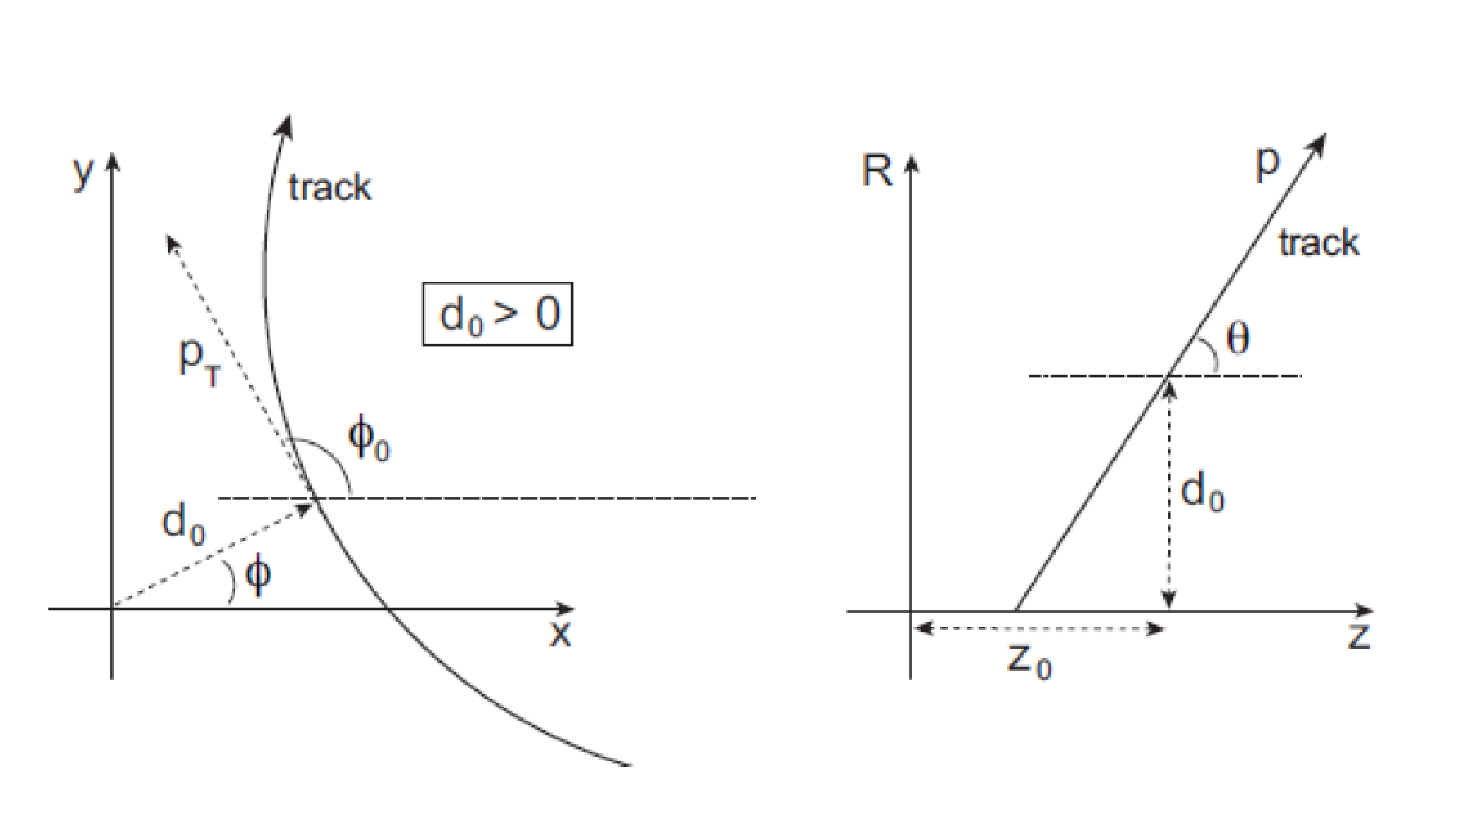
\includegraphics[width=0.7\textwidth]{objectsreconstruction/figures/tracks}}
	\caption{Schematic drawings of the parameters used for track reconstruction in the XY and $R$Z planes (left and right respectively).
          The parameters are: $q/p$, the charge divided by the momentum; $\theta$, or more used $\eta$, the angle
          with respect to the Z axis in the $R$Z plane measured from the perigee; $\phi_0$, the angle 
          with respect to the X axis in the XY plane measured from the perigee; $d_0$, the impact parameter, 
          or perigee with respect to the Z axis in the XY plane; $z_0$, Z component of the perigee.\label{fig:trackpar}}
\end{center}\end{figure}


Clusters are built starting from
$\Delta\eta\times\Delta\phi=0.025\times0.025$ single energy deposits summing
up into towers. Adjacent towers form clusters of $3\times7$ cells units in $\eta\times\phi$
in $|\eta|<1.4$ and $5\times5$ further.




excluding the transition region $1.37<|\eta| <1.52$
with inactive material.



%\section{Muons}\label{sec:muons}
\subsection{Muons}\label{sec:muons}



%\section{Jets}\label{sec:jets}
\subsection{Jets}\label{sec:jets}


%\section{Missing Transverse Energy}\label{sec:met}
\subsection{Missing Transverse Energy}\label{sec:met}


\clearpage{\pagestyle{empty}\cleardoublepage}
\phantomsection
\addcontentsline{toc}{chapter}{Part II}
\input{smallstuff/pII.tex}
%\chapter*{Part II}
\clearpage{\pagestyle{empty}\cleardoublepage}
\clearpage{\pagestyle{empty}\cleardoublepage}

\chapter{Searches for vector-like top partner pairs in the single lepton channel}~\label{chap:vlq}

In the following Chapter we will describe two searches for vector-like 
top partners \TTbar\ pairs performed in the single 
lepton\footnote{From now on, with the word ``lepton'' we will 
mean only either electron or muon, assumed to come from the leptonic
decay of a $W$ boson with its associated neutrino, which is considered
to be the only particle contributing to the transverse missing energy \met.} channel. 
These analyses
are optimized for different final states and are thus complementary.
The first search focuses on decay channels with high BR to $Wb$ and is 
performed using the full dataset of p-p collisions at the \cme of \rts=8~\tev\
collected during 2012 at the ATLAS detector, consinsting in 20.34~\ifb, while
the preliminary search for vector-like top partners with high BR to $Ht$
uses a partial dataset of the same data, amounting to 14.3~\ifb.

The Chapter is organized as follows: first Section~\ref{sec:presel}
introduces the common event preselection for data and few general concepts in the
analyses design; Section~\ref{sec:MCbkg}
presents the Monte Carlo samples used in the searches, which
are in general common to both analyses with only few exceptions that are reported;
Section~\ref{sec:qcdbkg} describes how the multi-jet background from QCD events is
obtained.
Finally, the two analyses are detailed in Section~\ref{sec:wbx} and Section~\ref{sec:htx}, 
which illustrate the event selection criteria, the background modeling estimation, 
the systematics affecting the analysis, the statistical treatment and the
results.

\section{Data sample and common event preselection}\label{sec:presel}

The data from p-p collision events recorded at the ATLAS experiment during
2012 at a \cme\ of $\rts=8\tev$ are considered. Physics object definitions 
were previously discussed in Section~\ref{sec:objects}.
Events collected during
stable beam periods are required to pass data quality requirements and
single lepton trigger selection. In order to maximize trigger
efficiency, different transverse momentum threshold triggers are combined
through a logical \OR, with the lower \pt\ ones including isolation requirements
that result in inefficiencies for high \pt\ lepton candidates, recovered with
the use of the higher threshold triggers. The electron triggers have
\pt\ thresholds of 24 and 60\gev, the muon ones of 24 and 36\gev.

After passing trigger requirements, events with more than one lepton are
discarded. In addition, the only lepton of the event has to match within $\dr<0.15$ the
triggered one. As basic preselectio, four jets satisfying the conditions
described in Section~\ref{sec:jets} are required, at least one of them
being tagged as a \bjet.

In order to suppress the multi-jet background from QCD processes,
combined cuts on the \met\ and on the tranverse mass of the 
leptonically decaying $W$ boson \mt\footnote{$\mt = \sqrt{2 p^\ell_{\rm T} \met (1-\cos\Delta\phi)}$, with
$p^\ell_{\rm T}$  being the transverse momentum (energy) of the muon (electron) and $\Delta\phi$ the
azimuthal angle separation between the lepton and the direction of
the missing transverse momentum.}\ 
are defined: $\met>20~\gev$ and $\met+\mt>60~\gev$.

At this point, a simple consideration about the typical expected jet
(and \bjet) multiplicity is made so as to define an orthogonality
cut between the two analyses. Table~\ref{tab:jetmult} shows the 
number of jets (\bjet s) per decay channel combinations of \TTbar\ pairs, 
in the case of single lepton selection with at least four jets
(i.e. one $W$ boson will always decay into lepton and neutrino,
and $Z$ boson decay to neutrinos is excluded in the $WbZt$ channel) and assuming that
the Higgs boson decays to a bottom quark-antiquark pair.
To avoid overlap between selected events from the two analyses, in the
\wbx\ analysis events with $\geq$6 jets and $\geq$3 \bjet s are 
rejected\footnote{As will be explained later in Section~\ref{sec:htxEVT}, another orthogonality
cut will be applied in the low \bjet\ multiplicity channel of the \htx\ analysis.}.

\begin{table}\centering
	\begin{tabular}{lccc}\toprule
	 & $Wb$ & $Ht$ & $Zt$ \\\midrule
             &\cellcolor{lightgray} & & \cellcolor{lightgray}\\
	\multirow{-2}{*}{$Wb$} & \cellcolor{lightgray}\multirow{-2}{*}{\bf 4 (2)} & \multirow{-2}{*}{6 (4)} & \cellcolor{lightgray}\multirow{-2}{*}{{\bf 6} ({\bf2}/4)} \\
        \multirow{2}{*}{$Ht$} & \multirow{2}{*}{6 (4)} & \multirow{2}{*}{8 (6)} & max: 8 (4/6)\\
             & & & \cellcolor{lightgray}min: {\bf6 (2)}\\
        \multirow{2}{*}{$Zt$} & \cellcolor{lightgray}& max: 8 (4/6) & \cellcolor{lightgray}max: {\bf8} ({\bf2}/6) \\
             & \cellcolor{lightgray}\multirow{-2}{*}{\bf6 (2/4)} & \cellcolor{lightgray}min: {\bf6 (2)} & \cellcolor{lightgray}min: {\bf6} ({\bf2}/4)\\
	\bottomrule\end{tabular}\caption{Jets (\bjet s) multiplicities in the various possible final states. $Z$ boson decays 55\% hadronically, 15\% of the 
        times into \bbbar, therefore the min/max number of \bjet s is reported. Highlighted are the channels that after the orthogonality cut
        will contribute to the \wbx\ analysis.}\label{tab:jetmult}
\end{table}




\section{Background and signal modeling}\label{sec:datasets}

The main background for both analyses is $t\bar{t}$ 
production with jets ($t\bar{t}$+jets in the following) 
and different choices for the generator are made
in the analyses because of the specific needs of having well
modeled regions.
In the case of the $t\bar{t}$+jets background prediction for the \htx\ analysis 
further corrections to match the data are applied, due to a mismodeling in the
heavy- and light-flavour content of the simulated sample (see Section~\ref{sec:htxEVT}).

$W$ boson production  in association with jets ($W$+jets in the following) 
and multi-jet events from QCD processed also contributes, the latter
sneaking into the event selection via the misidentification of a jet or a photon as an
electron or the presence of a non-prompt lepton from, e.g., semileptonic $b$- or $c$-hadron decay.
Other background smaller components are single top quark, $Z$+jets, diboson
($WW,WZ,ZZ$), and $t\bar{t}$ production associated with a vector or Higgs boson.

All event generators using {\sc Herwig}~\cite{herwig} are also interfaced to {\sc
Jimmy} v4.31~\cite{jimmy} to simulate the underlying event.  
With the exception of the 
signal samples, all simulated 
samples utilise {\sc Photos 2.15}~\cite{PhotosPaper} to model
photon radiation and {\sc Tauola 1.20}~\cite{TauolaPaper} to model
$\tau$ decays.  

All simulated samples include multiple p-p
interactions and go through the  {\sc Geant4}~\cite{geant}
detector geometry and response simulation~\cite{atlas_sim}
with the exception of the signal samples, for which a fast simulation of
the calorimeter response is used.

All simulated samples are then processed through the same reconstruction 
software as the data and are reweighted to match 
the instantaneous luminosity profile in data. 

%Additional corrections are applied so that the 
%object identification efficiencies, energy
%scales and energy resolutions match those determined in data control
%samples.


\subsection{Monte Carlo simulated samples}\label{sec:MCbkg}

\subsubsection{$t\bar{t}$ MC@NLO}\label{subsec:MC@NLO}
Simulated samples of $t\bar{t}$ pair production  in association with jets 
($t\bar{t}$+jets or simply $t\bar{t}$ in the following)
are generated with {\sc MC@NLO} v4.01~\cite{mcatnlo_1,mcatnlo_2,mcatnlo_3} using the {\sc CT10} set of parton distribution functions (PDFs)~\cite{ct10},
with the parton-shower and fragmentation steps being performed by 
{\sc Herwig} v6.520~\cite{herwig}.
The top quark mass is assumed to be equal to $172.5\gev$ and 
the samples are normalized to approximate next-to-next-to-leading-order 
(NNLO) theoretical cross section~\cite{ttbarxs}; the cross section used 
has been computed with {\sc Hathor} 1.2~\cite{ttbarxs} using the {\sc MSTW2008}
NNLO PDF set~\cite{mstw} and is $\sigma_{t\bar{t}}= 238^{+22}_{-24}$~pb, 
where the total uncertainty results from the sum in quadrature of the 
scale and PDF+$\alpha_S$ uncertainties according to 
the {\sc MSTW} prescription~\cite{mstw2}. 
This is the $t\bar{t}$ used in the \wbx\ analysis.

\subsubsection{$t\bar{t}$ Alpgen}\label{subsec:alpgen}
Simulated samples of $t\bar{t}$+jets are generated using
%and $W/Z$+jets events are generated using
 the {\sc Alpgen v2.13}~\cite{alpgen} leading-order (LO) generator and the 
{\sc CTEQ6L1} PDF set~\cite{cteq6}, with parton shower and fragmentation  
modelled through {\sc Herwig} v6.520~\cite{herwig}.

A parton-jet matching scheme called ``MLM matching''~\cite{mlm} is used
in orderd to avoid double-counting  of partonic configurations
eventually generated both at the matrix-element calculation level
and at the parton-shower evolution step.

Separate samples are generated for $t\bar{t}$+light jets ($t\bar{t}$+light 
or $t\bar{t}$+LF in the following, from ``light flavour'') 
with up to three additional light partons ($u$, $d$, $s$ quarks or gluons),
and for $t\bar{t}$+heavy-flavour jets ($t\bar{t}$+HF in the following), 
including $t\bar{t}b\bar{b}$ and
$t\bar{t}c\bar{c}$.  
An algorithm based on the angular separation
between the extra heavy quarks is used to remove 
the overlap between $t\bar{t}q\bar{q}$ ($q=b,c$) 
generated from the matrix element calculation and 
from parton-shower evolution in the  $t\bar{t}$+light samples
is employed: matrix-element prediction is chosen over the parton-shower one
when $\Delta R(q,\bar{q})>0.4$, else vice-versa.

%The algorithm used is implemented in the HFOR tool~\cite{hfor}.

Again a top quark mass of $172.5\gev$ is assumed, and normalisation to the
NNLO theoretical cross section is used (see~\ref{subsec:MC@NLO})

\subsubsection{$W/Z$+jets}

Simulated samples of $W/Z$ boson production in association with jets
($W/Z$+jets in the following) are generated with up to five additional 
partons using the {\sc Alpgen v2.13}~\cite{alpgen} LO generator and the 
{\sc CTEQ6L1} PDF set~\cite{cteq6}, interfaced to {\sc Herwig} v6.520 
for parton showering and fragmentation.

``MLM matching'' is used also here to avoid double-counting of partonic configurations 
between  matrix-element  calculation and parton showering.

The $W$+jets samples are generated separately for $W$+light jets, 
$Wb\bar{b}$+jets, $Wc\bar{c}$+jets, and $Wc$+jets, 
with the relative contributions normalized using the fraction 
of $b$-tagged jets in $W$+1-jet and $W$+2-jets data 
control samples~\cite{whf}, while
the $Z$+jets samples are generated separately 
for $Z$+light jets, $Zb\bar{b}$+jets, and $Zc\bar{c}$+jets and
normalized to the inclusive NNLO theoretical cross section~\cite{vjetsxs}.

Overlap between $W/Zq\bar{q}$+jets ($q=b,c$) 
events generated from the matrix element calculation and those
generated from parton-shower evolution in the $W/Z$+light jets
samples is avoided via an algorithm analogous to the one used
for $t\bar{t}$ Alpgen.

For the $W$+jets background, a normalisation from data for the shapes 
obtained from the simulation is derived since the simulation 
overestimates the number of $W$+jets events
by up to $\sim$20\%, depending on the jet multiplicity.

By exploiting the predicted asymmetry between
$W^+$+jets and $W^-$+jets production in p-p collisions~\cite{wasym},
the total number of $W$+jets events in data ($N_W=N_{W^+}+N_{W^-}$), 
can be estimated based on the measured
difference between the number of positively- and negatively-charged $W$
bosons, $(N_{W^+}-N_{W^-})_{\rm meas}$, and the asymmetry predicted from the simulation:
\begin{equation}
N_W = \left(\frac{N_{W^+}+N_{W^-}}{N_{W^+}-N_{W^-}}\right )_{\rm MC}(N_{W^+}-N_{W^-})_{\rm meas}
\label{eq:nw}
\end{equation}

Events are categorised in terms of  multiplicity of $b$ and $c$ jets and scale factors are
derived using Equation~\ref{eq:nw}.
The fraction of $W$+light jets events is scaled accordingly
in order to preserve the overall normalisation of the $W$+jets background before $b$ tagging.


\subsubsection{Other backgrounds}\label{subsec:otherbkg}
%,tchanxs,Wtchanxs,schanxs}. 
Simulated samples of single top quark backgrounds corresponding to the
$s$-channel and $Wt$ production mechanisms are generated with {\sc
MC@NLO} v4.01~\cite{mcatnlo_1,mcatnlo_2,mcatnlo_3} using the {\sc
CT10} PDF set~\cite{ct10}.  In the case of $t$-channel single top
quark production, the {\sc AcerMC} v3.8 LO generator~\cite{acermc}
with the {\sc MRST LO**} PDF set is used.

Simulated samples of $t\bar{t}$ produced in association with a $W$ or $Z$ boson
($t\bar{t}V$ $(V=W,Z)$ in the following) are generated with the {\sc Madgraph v5} LO
generator~\cite{madgraph} and the {\sc CTEQ6L1} PDF set.  

Samples of $t\bar{t}$ produced in association with a Higgs boson
($t\bar{t}H$ in the following) are generated with the 
{\sc Pythia} 6.425~\cite{py6} LO generator and the {\sc MRST LO**} PDF set~\cite{mrst},
assuming a Higgs boson mass of $125\gev$ and considering the 
$H\to b\bar{b}$, $c\bar{c}$, $gg$, and $W^+W^-$ decay modes.

Parton shower and fragmentation are modelled with {\sc Herwig}
v6.520~\cite{herwig} in the case of {\sc MC@NLO}, with {\sc Pythia}
6.421 in the case of {\sc AcerMC}, and with {\sc Pythia} 6.425 in the
case of {\sc Madgraph}.  All these samples are generated assuming a top
quark mass of $172.5\gev$. The single top quark samples are normalised to
the approximate NNLO theoretical cross sections~\cite{stopxs,stopxs_2}
using the {\sc MSTW2008} NNLO PDF set, while the $t\bar{t}V$ samples
are normalised to the NLO cross section predictions~\cite{ttbarVxs1,ttbarVxs2}.
The $t\bar{t}H$ sample is normalised using the NLO theoretical cross section 
and branching ratio predictions~\cite{lhcxs}.
Finally, the diboson backgrounds are modelled using {\sc Herwig} with
the {\sc MRST LO**} PDF set, and are normalised to their NLO
theoretical cross sections~\cite{dibosonxs}.

\subsubsection{Signal samples}\label{subsec:MCsignal}


For vector-like $T$ signals, samples corresponding to a singlet $T$ quark 
decaying to $Wb$, $Zt$ and $Ht$ are generated with the {\sc Protos} v2.2 
LO generator~\cite{jaas,protos} 
using the  {\sc MSTW2008} LO PDF set, and interfaced to {\sc Pythia} for 
the parton shower and fragmentation. 

For each decay channel ($Wb$, $Zt$ and $Ht$) the branching ratio has been 
set to 1/3. Events are reweighted
in order to reproduce any desired branching ratio configuration. 

The predicted branching ratios in the weak-isospin singlet and doublet scenarios as 
a function of $m_{T}$ are given in Table~\ref{tab:BRT}.

The $m_{T}$ values considered range from $350\gev$ to $850\gev$ in steps of $50\gev$, 
with the Higgs boson mass assumed 
to be $125\gev$. All Higgs boson decay modes are considered, 
with branching ratios as predicted by {\sc hdecay}~\cite{hdecay}.

Signal samples are normalized to the approximate NNLO theoretical cross sections~\cite{ttbarxs} using the {\sc MSTW2008} NNLO PDF set.
The cross section values used are summarized in Table~\ref{tab:sigmaTT}.



\begin{table}[h!]
\begin{center}
\begin{tabular}{c c c c c c c}
\hline
\hline
 & \multicolumn{3}{c}{Singlet} &  \multicolumn{3}{c}{Doublet} \\
 $m_{T}$ ($\gev$) & $BR(T \to Wb)$ & $BR(T \to Zt)$ & $BR(T \to Ht)$ & $BR(T \to Wb)$ & $BR(T \to Zt)$ & $BR(T \to Ht)$\\
\hline
350 	&  0.545 	&  0.116 	&  0.338	&  0.000 	&  0.255 	&  0.745 	\\ 
400 	&  0.513 	&  0.139 	&  0.348	&  0.000 	&  0.285 	&  0.715 	\\
450 	&  0.502 	&  0.158 	&  0.341	&  0.000 	&  0.316 	&  0.684 	\\ 
500 	&  0.497 	&  0.173 	&  0.330	&  0.000 	&  0.343 	&  0.657 	\\
550 	&  0.495 	&  0.185 	&  0.321	&  0.000 	&  0.365 	&  0.635 	\\
600 	&  0.494 	&  0.194 	&  0.312	&  0.000 	&  0.383 	&  0.617 	\\ 	
650 	&  0.494 	&  0.202 	&  0.304	&  0.000 	&  0.399 	&  0.601 	\\ 
700 	&  0.494 	&  0.208 	&  0.298	&  0.000 	&  0.411 	&  0.589 	\\ 
750 	&  0.494 	&  0.214 	&  0.292	&  0.000 	&  0.422 	&  0.578 	\\ 
800 	&  0.494 	&  0.218 	&  0.288	&  0.000 	&  0.431 	&  0.569 	\\
850 	&  0.494 	&  0.222 	&  0.284	&  0.000 	&  0.439 	&  0.561 	\\ 
\hline
\hline
\end{tabular}
\caption{\label{tab:BRT} Branching ratios for $T$ decay as a function
of $m_{T}$ as computed with {\sc Protos} in the weak-isospin singlet and doublet scenarios.}
\end{center}
\end{table}
%%%%%%%%
\begin{table}[h!]
\begin{center}
\begin{tabular}{c c c c c}
\hline
\hline
 $m_{T}$ ($\gev$) & $\sigma(TT)$ (pb) & Scale uncertainties (pb) & PDF+$\alpha_s$ uncertainties (pb) & Total uncertainty (pb)\\
\hline
350 	&  5.083 		&  +0.140/-0.285 		&  + 0.569/-0.488 		&  +0.586/-0.565		\\
400 	&  2.296 		&  +0.066/-0.130 		&  + 0.269/-0.221 		&  +0.277/-0.257		\\
450 	&  1.113 		&  +0.034/-0.063 		&  + 0.136/-0.107 		&  +0.140/-0.125		\\
500 	&  0.5702 		&  +0.0185/-0.0327 		&  + 0.0723/-0.0545	 	&  +0.0746/-0.0636		\\
550 	&  0.30545 	&  +0.01040/-0.01769 	&  + 0.04012/-0.02889 	&  +0.0414/-0.0339		\\
600 	&  0.1696 		&  +0.0060/-0.0099 		&  + 0.0230/-0.0161	 	&  +0.0238/-0.0189		\\	
650 	&  0.09707 	&  +0.00359/-0.00571 	&  + 0.01363/-0.00936 	&  +0.01410/-0.01097	\\
700 	&  0.05694 	&  +0.00218/-0.00338 	&  + 0.00828/-0.00559 	&  +0.00856/-0.00653	\\
750 	&  0.03411 	&  +0.00135/-0.00204 	&  + 0.00513/-0.00343 	&  +0.00530/-0.00400	\\
800 	&  0.02080 	&  +0.00085/-0.00126 	&  + 0.00329/-0.00216 	&  +0.00340/-0.00250	\\
850 	&  0.01287 	&  +0.00054/-0.00079 	&  + 0.00215/-0.00138 	&  +0.00222/-0.00159 	\\
\hline
\hline
\end{tabular}
\caption{\label{tab:sigmaTT} Theoretical cross section at NNLO  for $TT$ production as a function
of $m_{T}$ as computed by {\sc Hathor}, and scale and PDF uncertainties.}
\end{center}
\end{table}
%%%%%%%%

\subsection{Multi-jet background}\label{sec:qcdbkg}

QCD production can pass the event selection in the electron
channel as non-prompt electrons or as ``fake'' electrons, i.e.
either electrons from photon conversions or mis-identified jets
that left a high amount of energy in the electromagnetic calorimeter.
For events in the muon channel the main contributions come from
non-prompt leptons from semileptonic $b$- and $c$-hadron decays.


The contribution to the background from multi-jet events is
estimated via data-driven methods, since
simulation is not expected to predict this contribution
with the desired level of accuracy.
The technique used is called ``Matrix Method'' (MM in the following)~\cite{ttbar_3pb}.  


\section{Search for \TTbar\ pairs decaying to $Wb+X$}\label{sec:wbx}

\subsection{Boosted $W$ reconstruction}\label{subsec:boostedW}

\subsection{Control regions}\label{sec:wbxCR}

\subsection{Event selection}\label{sec:wbxEVT}

%\subsection{}\label{sec:}

%\subsection{}\label{sec:}

\subsection{Systematics}\label{sec:wbxSYS}



\section{Preliminary search for \TTbar\ pairs decaying to $Ht+X$}\label{sec:htx}

\subsection{Control regions}\label{sec:htxCR}

\subsection{Event selection}\label{sec:htxEVT}

%\subsection{}\label{sec:}

%\subsection{}\label{sec:}

\subsection{Systematics}\label{sec:htxSYS}



\clearpage{\pagestyle{empty}\cleardoublepage}
\clearpage{\pagestyle{empty}\cleardoublepage}

\chapter{Preliminary search for \TTbar\ pairs decaying to $Wb+X$}\label{chap:wbx}

\section{Boosted $W$ reconstruction}\label{sec:boostedW}

\section{Control regions}\label{sec:wbxCR}

\section{Event selection}\label{sec:wbxEVT}

%\section{}\label{sec:}

%\section{}\label{sec:}

\section{Systematics}\label{sec:wbxSYS}


\clearpage{\pagestyle{empty}\cleardoublepage}
\clearpage{\pagestyle{empty}\cleardoublepage}

\chapter{Preliminary search  for \TTbar\ pairs decaying to $Ht+X$}\label{chap:htx}

\section{Control regions}\label{sec:htxCR}

\section{Event selection}\label{sec:htxEVT}

%\section{}\label{sec:}

%\section{}\label{sec:}

\section{Systematics}\label{sec:htxSYS}



%%%%NB COPY PASTE
The total prior systematic uncertainty
in the background normalisation in the $\geq 4$ $b$-tags channel is 
$\sim$42\%, with the dominant uncertainties being from $b$ tagging efficiency (16\%),
$c$ tagging efficiency (11\%), jet energy scale (11\%), $t\bar{t}$ modelling (11\%), 
$t\bar{t}$+heavy-flavour fractions (32\%) and $t\bar{t}$ cross section (10\%).
As a result of the two-parameter fit, the total background uncertainty is reduced 
by about 80\% in this channel. The total  systematic uncertainty
in the signal normalisation in the $\geq 4$ $b$-tags channel is 
$\sim$21\%, completely dominated by the uncertainty in the $b$ tagging efficiency.


\clearpage{\pagestyle{empty}\cleardoublepage}
\clearpage{\pagestyle{empty}\cleardoublepage}

\chapter{Final results}\label{chap:results}

Through Chapters~\ref{chap:vlq},~\ref{chap:wbx} and~\ref{chap:htx}
we presented the strategy adopted for the searches of vector-like
top partners in the single lepton channel and implemented into
two complementary analyses: the \wbx\ and the \htx\ analyses.
Each of these analyses is probing a different
area of the two-dimensional plane (described in Section~\ref{sec:strategy}) 
defined in order to perform
a model-independent scan of the three possible decay channels BR 
mixing phase space.
In this chapter we are going to illustrate how the results
obtained by the individual analyses (Sections~\ref{sec:wbxRES} 
and~\ref{sec:htxRES}) perform when the search channels are
combined (Section~\ref{sec:results_comb}).
In Section~\ref{sec:coverage} we compare
the coverage of the BRs two-dimensional
mixing plane by the four quasi-model independent
searches for vector-like quarks performed
by the Exotics group.


\section{Combination of the \wbx\ and \htx\ analyses}\label{sec:results_comb}

As the \wbx\ and the \htx\ analyses do not overlap
thanks to the orthogonality requirements (rejection of
events with $\geq$ 6 jets and $\geq$ 3 \btag ged jets
in the \wbx\ analysis, rejection of events with $H_T>700~\gev$
in the \chii\ channel of the \htx\ analysis), it is possible
to obtain a fully combined result. Figure~\ref{fig:searchchan}
reports the final search channels to be used.

\begin{figure}[h!tb]\begin{center}
	\subfigure[]{\label{fig:htx2}
%\includegraphics[width=0.45\textwidth]{htx_analysis_14ifb/figures/final/HTAll_6jetin2btagex_ELEMUON.eps}}
\includegraphics[width=0.45\textwidth]{results/figures/THESIS_c8_signal/HTAll_6jetin2btagex_ELEMUON.eps}}
	\subfigure[]{\label{fig:htx3}
%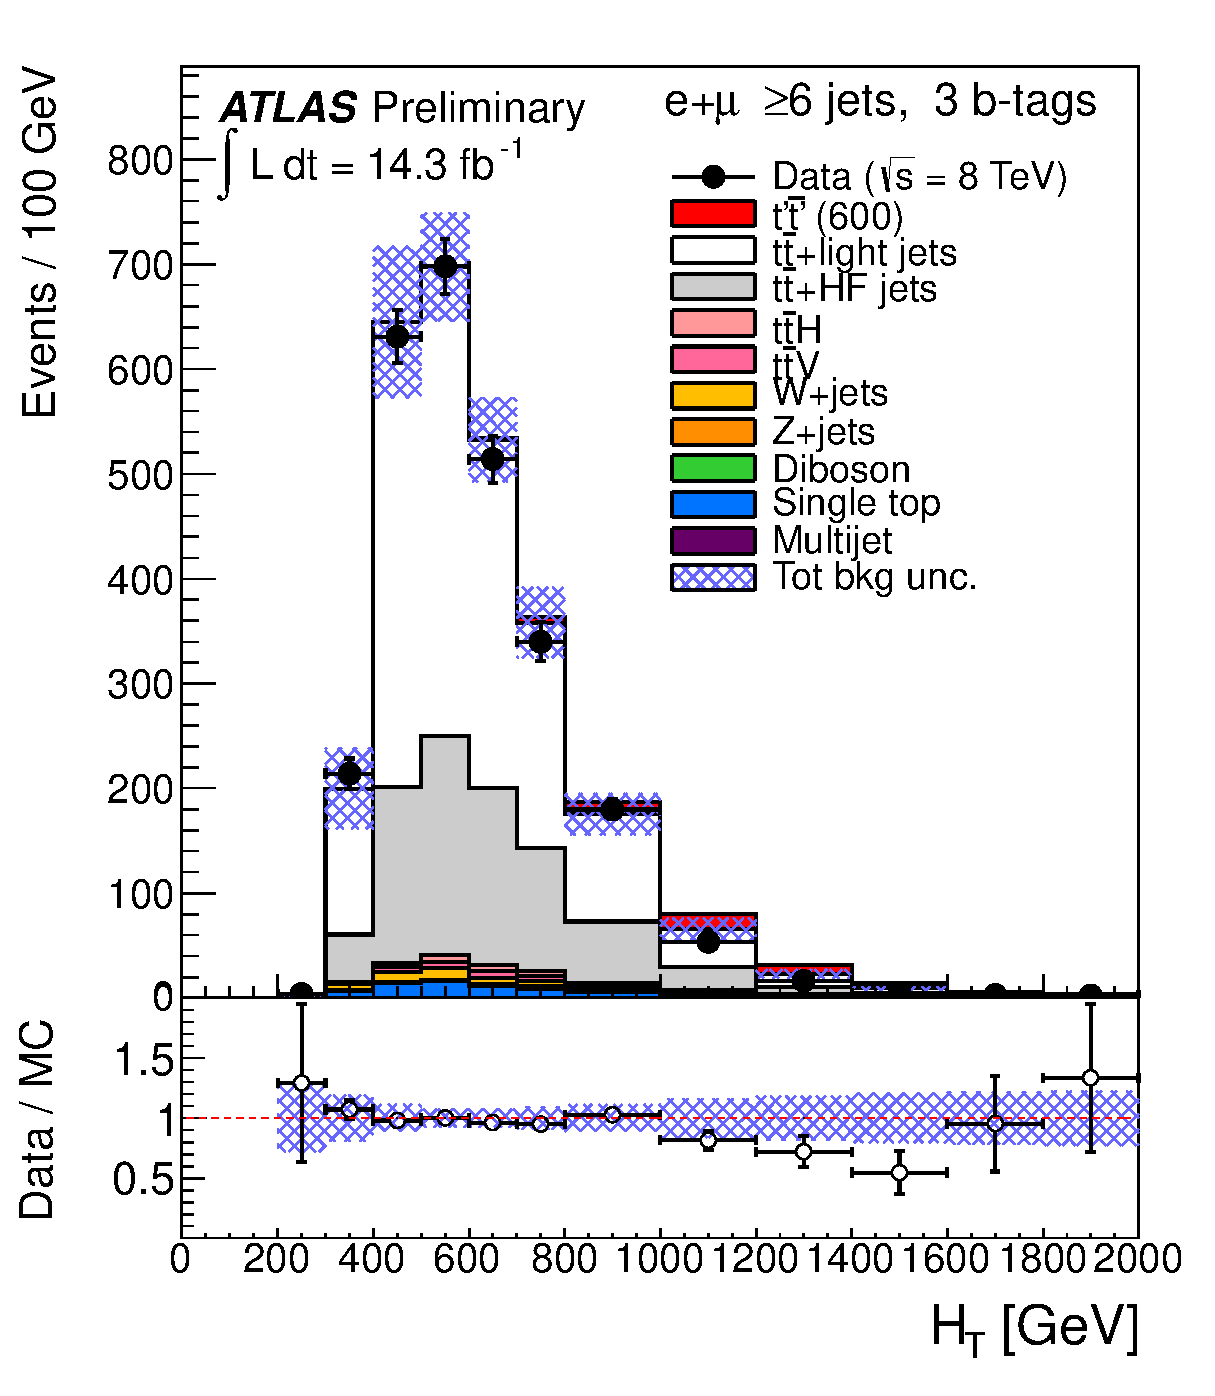
\includegraphics[width=0.45\textwidth]{htx_analysis_14ifb/figures/final/HTAll_6jetin3btagex_ELEMUON.eps}}
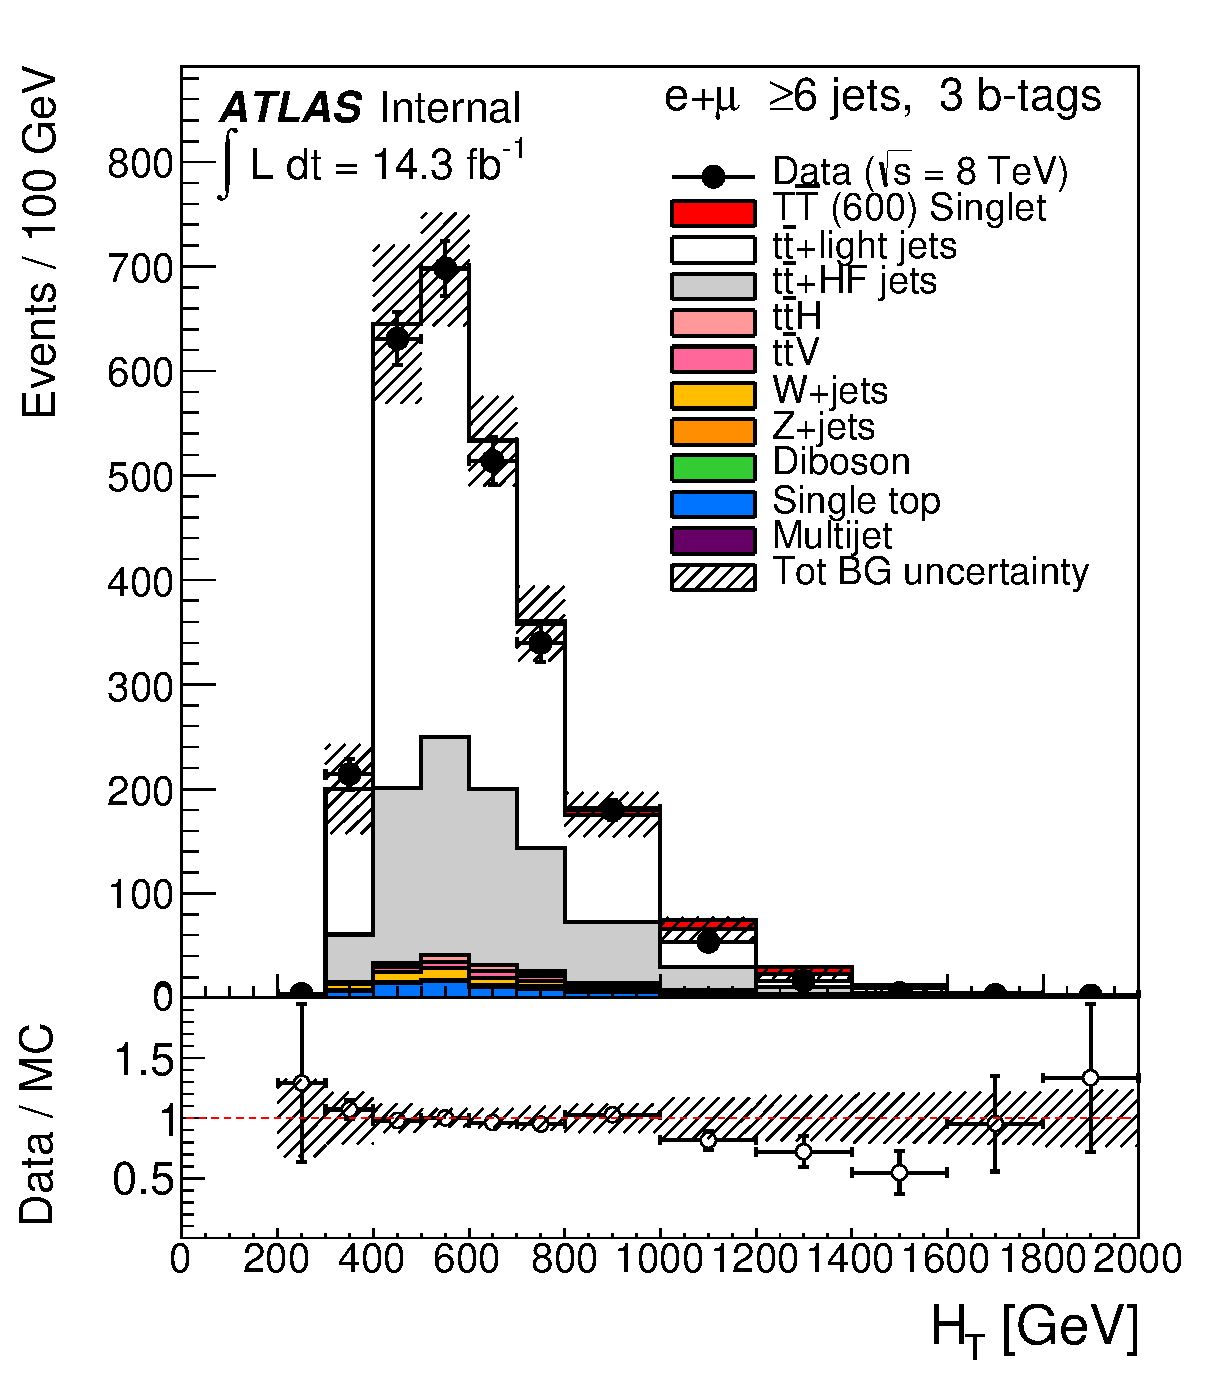
\includegraphics[width=0.45\textwidth]{results/figures/THESIS_c8_signal/HTAll_6jetin3btagex_ELEMUON.eps}}
	\subfigure[]{\label{fig:htx4}
%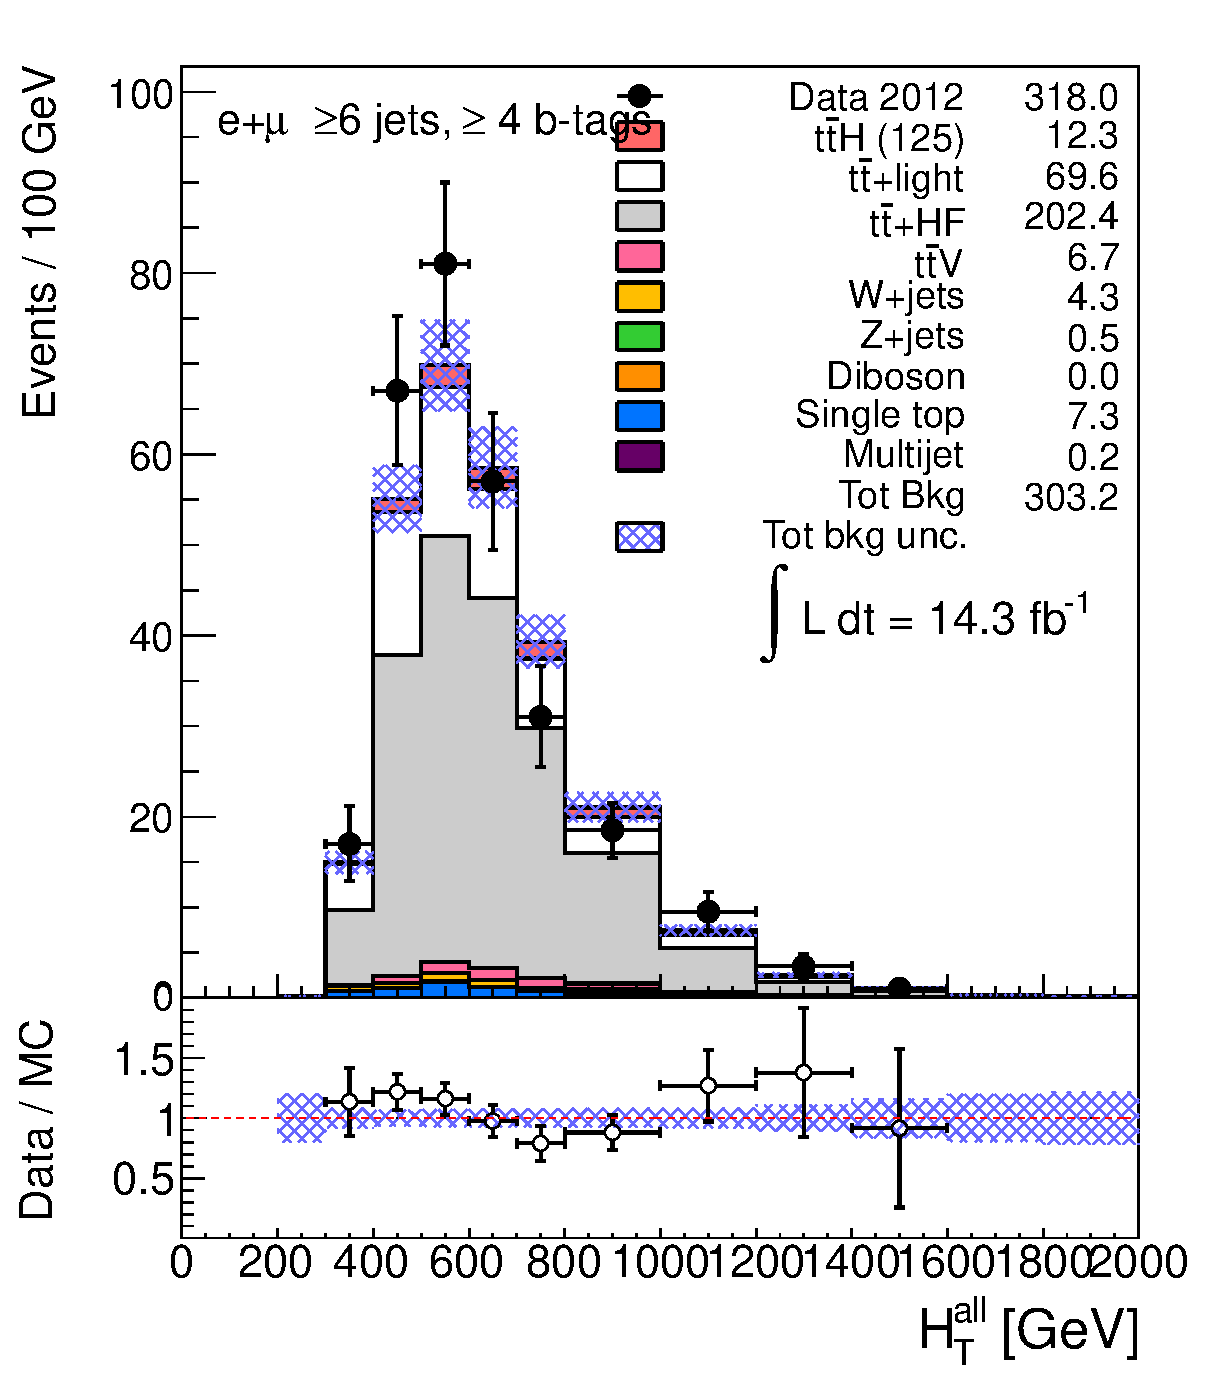
\includegraphics[width=0.45\textwidth]{htx_analysis_14ifb/figures/final/HTAll_6jetin4btagin_ELEMUON.eps}}
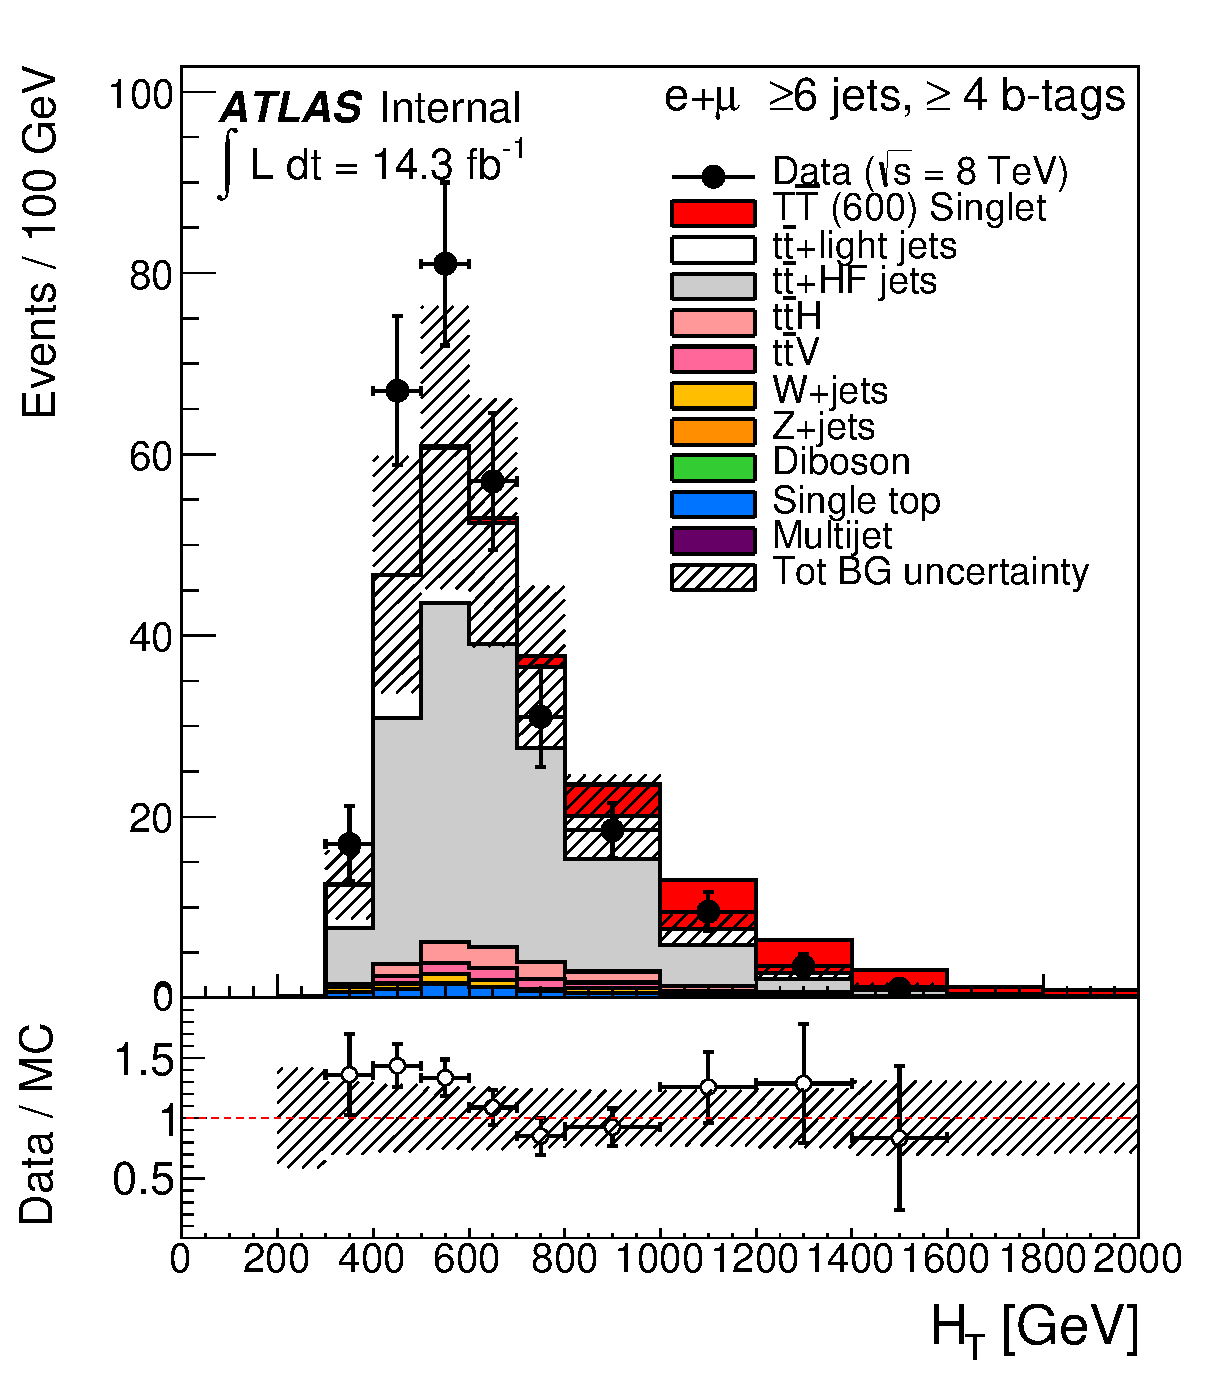
\includegraphics[width=0.45\textwidth]{results/figures/THESIS_c8_signal/HTAll_6jetin4btagin_ELEMUON.eps}}
	\subfigure[]{\label{fig:wbx1}
%\includegraphics[width=0.45\textwidth]{wbx_analysis_14ifb/figures/confnoteplots/VLQAna_WbX_1W_MWb_4_ELEMUON_cutflow1234567_NOMINAL.eps}}
\includegraphics[width=0.45\textwidth]{results/figures/THESIS_c8_signal/VLQAna_WbX_1W_MWb_4_ELEMUON_cutflow1234567_NOMINAL.eps}}
	\caption{Final discriminant variables distributions in the search channels
        of the \htx\ analysis ($\HT$ in (a) \chii, (b) \chiii\ and (c) \chiv\ channels)
        and of the \wbx\ analysis (\mreco\ in the \tight\ channel). In all plots the
        signal is shown for the singlet model. The uncertainty bands include statistical 
        and systematic uncertainties.\label{fig:searchchan}}
\end{center}\end{figure}

For the purpose of a combined statistical analysis
of the four channels,
choices on the systematic 
uncertainties treatment have to be done.
Uncertainties that are common to both analyses and that
are treated in the same way are considered as fully 
correlated and are: integrated luminosity; lepton reconstruction, 
identification and trigger (1 component); jet vertex fraction;
jet energy resolution;
$b$ tagging (9 components); $c$ tagging (5 components); light-jet 
tagging (1 component);
background cross sections ($t\bar{t}$, single top, diboson, $t\bar{t}V$).
For the JES uncertainty, while the \wbx\ analysis considers a single component
the \htx\ uses the 8 components breakdown and is then impossible to 
correlate the individual JES uncertainty sources one by one.
Since in the \htx\ analysis the dominant JES uncertainty eigenvector is the BASELINE
(see Section~\ref{sec:htxSYS}) the choice is to correlate the \wbx\ analysis JES 
uncertainty with the BASELINE uncertainty of the \htx\ analysis.
The systematic uncertainties that are not taken as correlated are:
$W$+jets normalization, divided into 5 components in the \wbx\ 
analysis and only 1 in the \htx\ analysis where, however, is a negligible 
background; $t\bar{t}$ modeling, as the two analyses use different $t\bar{t}$ 
Monte Carlo generators and probe very different
final state kinematics region with different flavor composition.

The benchmark model chosen to show the exclusion limit as a function
of the mass is the vector-like singlet $T$ quark scenario, as
it is the common benchmark model for the two analyses. In this
case the \htx\ analysis performed better than the \wbx\ analysis,
giving an  observed (expected) 95\%  CL  limit value of
$m_{\T}>640\,(615)\gev$.
Figure~\ref{fig:limits1D_combo} shows the observed and expected 
upper limits on the \TTbar\ production cross section 
times branching fraction as a function of $m_{\T}$ for a weak-isospin
singlet  after combination of the two analyses.
The observed (expected) 95\% CL limit is 
$m_{\T}>670\,(675)\gev$ for the central value 
of the theoretical cross section,
improving by $\sim$30$\gev$ the expected sensitivity 
obtained by the \htx\ analysis alone.

\begin{figure}[h!tb]
\centering
\includegraphics[width=0.45\textwidth]{results/figures/lim_singlet_comb.eps} 
\caption[bla]{Observed (solid line) and expected (dashed line) 95\% CL upper limit on the $\T \bar{\T}$ cross section times branching fraction
for a vector-like singlet $\T$ quark  as a function of the $\T$ quark mass, resulting from the combination of
the \wbx\ and the \htx\ analyses.
The surrounding shaded bands correspond to the $\pm1$ and $\pm2$ standard deviations around the expected limit. 
The thin red line and band show the theoretical prediction and its $\pm1$ standard deviation uncertainty.

\label{fig:limits1D_combo}}
\end{figure}

Figure~\ref{fig:limits2D_combo} shows the two-dimensional BR plane for 
different values of $m_{\T}$ with the  resulting 95\% CL exclusion limits.
Comparing this result with the ones of Figures~\ref{fig:limits2D_wbx} 
and~\ref{fig:limits2D_htx} it is evident the improvement resulting
from the combination of the two analyses, covering a much larger
area than the simple addition of two individual ones.
From this picture, vector-like top partners are completely excluded
no matter of the model in the mass range from 350~\gev\ up to 550~\gev\ 
(almost up to 600~\gev).

\begin{figure}[h!bt]
\centering
\includegraphics[width=0.9\textwidth]{results/figures/lim_Scan2D_comb.eps}
\caption{
Observed (red filled area) and expected (red dashed line) 95\% CL exclusion in the plane of
$BR(\T \to Wb)$ versus $BR(\T \to Ht)$, for different values of the vector-like $\T$ quark mass.
The grey (dark shaded) area corresponds to the unphysical region where the sum of branching ratios exceeds unity. 
The default branching ratio values from the \texttt{PROTOS} event generator for the weak-isospin singlet and doublet cases 
are shown as plain circle and star symbols, respectively. This result  from the combination of
the \wbx\ and \htx\ analyses includes both statistical and systematic uncertainties.
\label{fig:limits2D_combo}}
\end{figure}

It is interesting to compare the 
combined result
of the \wbx\ and \htx\ analyses
of Figure~\ref{fig:limits2D_combo} 
with the separate analysis results
to understand the impact on sensitivity
of the statistical combination of
the search channels.
This comparison is presented in 
Figure~\ref{fig:limits2D_potentialcombo},
where the combined result is overlapped
to the two separate results in the BR
plane.
Looking e.g. at the 650~\gev\ mass point,
it can be clearly seen how the singlet
scenario, lying outside of the expected exclusion
region in the case of the single \htx\ analysis,
is then swallowed in the exluded area when
the same analysis is combined with the
\wbx\ analysis, which alone does not even
reach the proximities of that benchmark point.


\begin{figure}[h!bt]
\centering
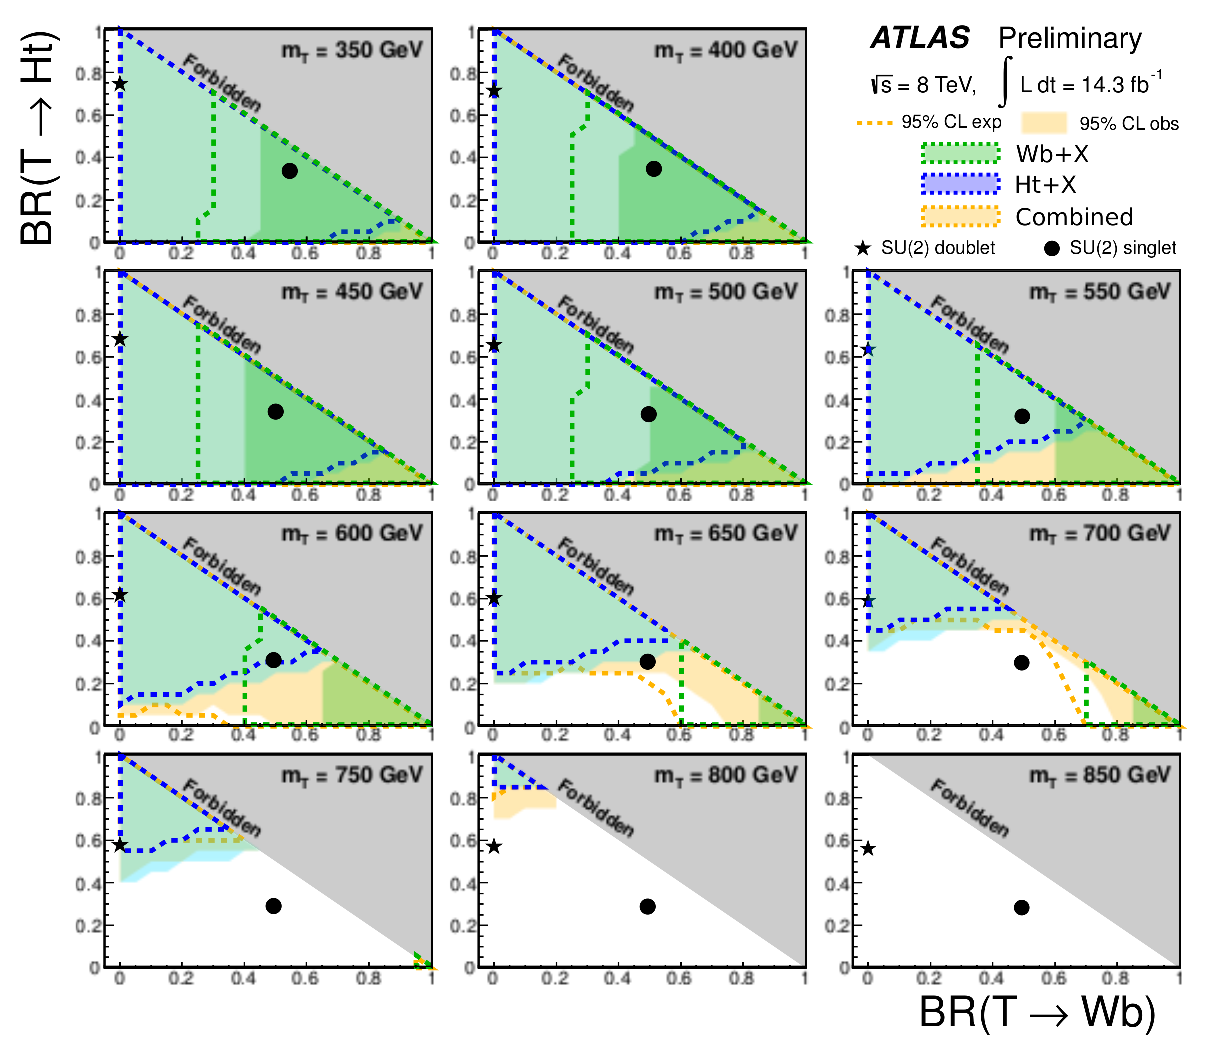
\includegraphics[width=0.9\textwidth]{results/figures/combinationoverlap.eps}
\caption{
Observed (filled area) and expected (dashed line) 95\% CL exclusion in the plane of
$BR(\T \to Wb)$ versus $BR(\T \to Ht)$, for different values of the $\T$ quark mass,
as result of the \wbx\ analysis (green), \htx\ analysis (blue), and the combination of the two (yellow).
The grey (dark shaded) area corresponds to the unphysical region where the sum of branching ratios exceeds unity. 
The default branching ratio values from the \texttt{PROTOS} event generator for the weak-isospin singlet and doublet cases 
are shown as plain circle and star symbols, respectively. All results
include both statistical and systematic uncertainties.
\label{fig:limits2D_potentialcombo}}
\end{figure}

\section{Comparison to other searches}\label{sec:coverage}

As briefly introduced in Section~\ref{sec:strategy}, two
additional analyses have been performed on the same dataset
as the \wbx\ and \htx\ analyses to search for heavy vector-like
top and bottom quarks in final states with exactly two leptons:
a search in the same-sign 
dilepton channel~\cite{ATLAS-CONF-2013-051} and 
a search in the opposite-charge dilepton channel~\cite{ATLAS-CONF-2013-056}.
It was shown that the four analyses probe different 
regions of the 2-dimensional mixing plane and are,
hence, complementary. Even though the single lepton and
the dilepton channels can be considered enough
separated, it was not possible to ensure a complete
orthogonality between all the analyses and they have
not, therefore, been combined\footnote{This
fact is mainly due to the different timescales
and frameworks at which the analyses have been developed. 
The \wbx\ and \htx\ searches
have been conceived to be combined since the
early stages of their design and were performed
inside the same analysis framework.}.
It is however useful to visualize how
the four searches contribute to the full
coverage of the BRs mixing plane by
observing Figure~\ref{fig:limits2D_allcombo}.
Here the results from the four searches,
each obtained independentely, are simply
overlapped. This picture corresponds somehow to
a ``worst case scenario'' of a possible
real combination of the four searches, as
in general the statistical analysis in the
case of additional signal enriched
channels would gain sensitivity. 
This can easily be grasped when looking
at the comparison between the combined result
of the \wbx\ and \htx\ analyses
with the plain overlap of the separate
coverages, shown in the previous section 
in Figure~\ref{fig:limits2D_potentialcombo}.

Figure~\ref{fig:limits2D_allcombo} shows that already
without combining any of the four searches,
\T\ quarks with masses up to 550~\gev, almost up
to 600~\gev, are excluded at 95\% CL without 
any assumption on the model. The same kind of
picture has been obtained in the BR plane for
\B\ quarks, shown in Figure~\ref{fig:limits2D_allvlb}.
Here the analyses contributing to the
95\% CL exclusion in the BR($B\to Hb$) vs  BR($B\to Wt$)
plane are the two searches in the multilepton channel.
The absence of a search probing the top-left corner
of the BR plane leaves for \B\ masses from 400~\gev up to
600~\gev only a very small area uncovered.


\begin{landscape}
\begin{figure}[h!bt]
\centering
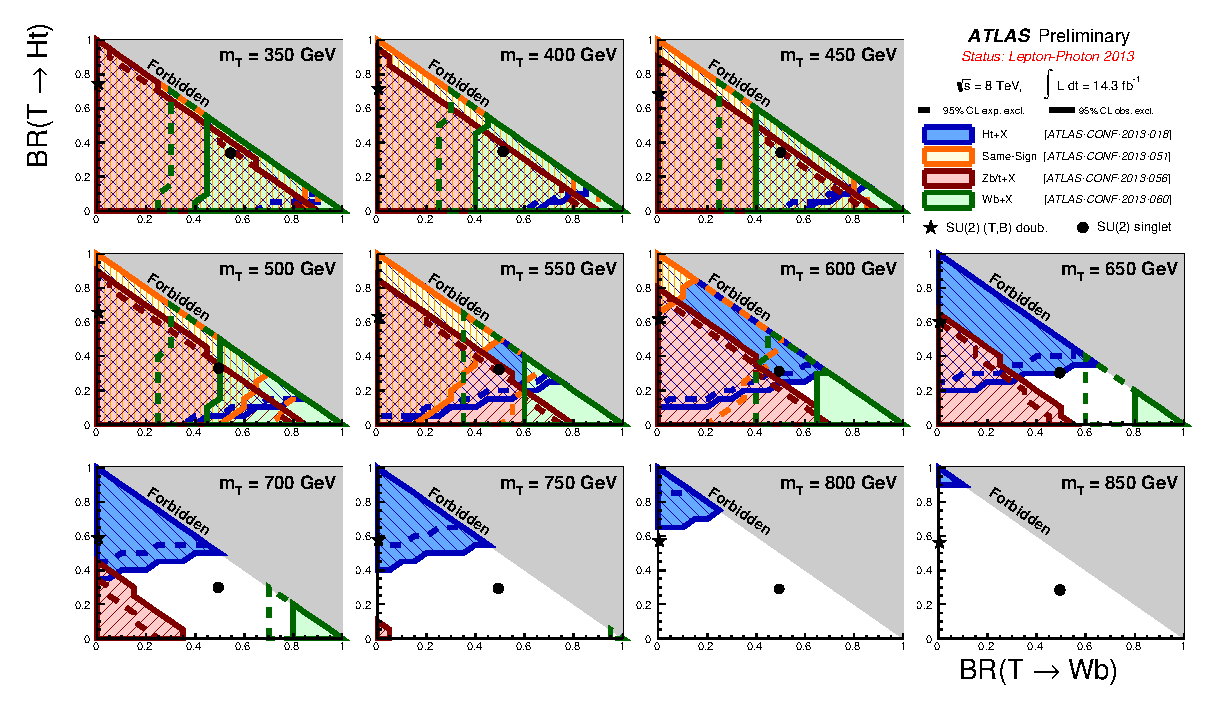
\includegraphics[width=1.5\textwidth]{results/figures/ATLAS_VLQ_TT_june2013_step4.eps}
\caption{
Observed (filled area) and expected (dashed line) 95\% CL exclusion in the plane of
$BR(\T \to Wb)$ versus $BR(\T \to Ht)$, for different values of the $\T$ quark mass.
In blue is shown the area excluded by the single lepton \htx\ analysis;
in orange is shown the area excluded by the same-sign dilepton analysis;
in red is shown the area excluded by the opposite-sign dilepton $\TTbar\to Zt+X$ analysis;
in green is shown the area excluded by the single lepton \wbx\ analysis.
The grey (dark shaded) area corresponds to the unphysical region where the sum of branching ratios exceeds unity. 
The default branching ratio values from the \texttt{PROTOS} event generator for the weak-isospin singlet and doublet cases 
are shown as plain circle and star symbols, respectively. This result includes both statistical and systematic uncertainties.
\label{fig:limits2D_allcombo}}
\end{figure}
\end{landscape}


\begin{landscape}
\begin{figure}[h!bt]
\centering
\includegraphics[width=1.5\textwidth]{results/figures/ATLAS_VLQ_BB_june2013_step2.eps}
\caption{
Observed (filled area) and expected (dashed line) 95\% CL exclusion in the plane of
$BR(\B \to Wt)$ versus $BR(\B \to Hb)$, for different values of the $\B$ quark mass.
In orange is shown the area excluded by the same-sign dilepton analysis;
in red is shown the area excluded by the opposite-sign dilepton $\TTbar\to Zt+X$ analysis.
The grey (dark shaded) area corresponds to the unphysical region where the sum of branching ratios exceeds unity. 
The default branching ratio values from the \texttt{PROTOS} event generator for the weak-isospin singlet and doublet cases 
are shown as plain circle and star symbols, respectively. This result includes both statistical and systematic uncertainties.
\label{fig:limits2D_allvlb}}
\end{figure}
\end{landscape}



\section{Outlook}\label{sec:combOUT}

At the time this dissertation is being
written, all of the four searches for
vector-like quarks are being updated to
the full available statistics of
pp collisions at \rts=8~\tev, about 20~\ifb,
for publication. The four searches maintain the
core strategies but have improvements in
background modeling (in particular with better
and more statistically populated Monte Carlo samples)
and reduced systematic uncertainties.
Searches in new channels are being developed, namely
$B\to Wt+X$ and $B\to Hb+X$, thus allowing for
the full coverage of the BR plane corners.
The complete plan for vector-like quark searches
in ATLAS is to combine all these analyses to 
achieve the highest sensitivity available.


\clearpage{\pagestyle{empty}\cleardoublepage}

\phantomsection
\addcontentsline{toc}{chapter}{Conclusions}
\clearpage{\pagestyle{empty}\cleardoublepage}

\chapter*{Conclusions and outlook}\label{chap:conclusions}

\vskip-1.5cm

Two quasi-model independent searches for 
pair production of vector-like top partners 
in proton-proton collisions at a \cme\ of 8~\tev\ 
have been presented in this dissertation. The final states considered
for both analyses involve one lepton and many jets but different
strategies are adopted in order to achieve sensitivities in different
corners of the decay phase space. Indeed, a peculiar fact for these
searches that has been stressed many times over these pages is the 
unpredicted nature of the heavy vector-like top partners model. 
As a direct consequence, the two analyses have been designed
and developed to be optimized for a particular decay mode and
to have orthogonal channels in order to allow
for a combined search that could exploit the specific sensitivities.

Three particular models, interesting from a theoretical point
of view (but not for this more favoured than others), are considered
over the two analyses: the chiral fourth-generation, with 
BR$(T\to Wb)=1$ for any value of the heavy quark mass; 
the singlet vector-like, with BR$(T\to Wb)\sim 0.5$ and 
BR$(T\to Ht)\sim 0.3$ for almost all
values of the heavy quark mass considered in the searches;
the doublet vector-like, with BR$(T\to Wb)= 0$ and 
BR$(T\to Ht)\in$ [0.50, 0.75] for all the values of the heavy quark mass.
In the \wbx\ analysis, it was possible to exclude at a 95\% CL
pair-produced chiral fourth-generation top partners and vector-like
$Y$ quarks with masses up to 740~\gev, and pair-produced vector-like 
singlet top partners with  masses up to 505~\gev.
In the \htx\ analysis, it was possible to exclude at a 95\% CL
pair-produced vector-like singlet and doublet top partners with 
masses up to 640~\gev\ and 790~\gev\ respectively.
When the two analyses are combined, the observed exclusion limit
for the only model where both analyses are sensitive, the
vector-like singlet $T$, is pushed $\sim$30~\gev\ further the
best result of the two, obtained by the \htx\ analysis,
achieving a 95\% CL exclusion of pair-produced vector-like singlet 
top partners with masses up to 670~\gev. While this might not
look like a significant improvement, the power of the combination
of the two searches is evident looking at the coverage of the
two-dimensional branching ratio plane, where  95\% CL exclusion is set for
pair-produced vector-like top partners with masses up to 550~\gev\ 
independently from the model, and also the plane for the 600~\gev\ mass
point is almost fully excluded. This strongly encourages to perform,
in the future, full combination of searches for vector-like quarks.

The mass range excluded at 95\% CL up to now
is getting closer and closer to the point where pair-production
of vector-like quarks will start to be disfavoured with respect
to single production. In this sense, while it is desirable to continue to
exploit the experience achieved up to now with the searches for
pair-produced vector-like quarks in the single lepton and multi-lepton
channels, it is a good idea to start designing searches for
single-produced vector-like quarks for LHC Phase-II.
Further improvements are possible for the searches
presented in this dissertation without changing the core of
the analysis strategies. During Phase-II they will benefit
of the increased \cme\ available for heavy quark production
in pp collisions with \rts=14~\tev\ and of the high integrated
luminosity (100~\ifb\ of data are expected over three years
of operation). With high luminosity comes the challenge of
dealing with higher pile-up, but considering that vector-like
quark searches involve high-\pt\ objects this should not
represent a major issue.

Besides the great discovery potential, the combination
of multiple searches will provide useful insights on the
exotic quark properties, like their quantum numbers or
the measurement of their branching ratios. 
Adding searches for single production of vector-like quarks
would also allow to measure the electroweak couplings of
these particles with the Standard Model quarks from the third generation.
Finally, these searches are even more interesting since
they will probe a wide range of
signatures that are often shared with other new physics
scenarios. Given the fact that during these last successful years
of LHC operation no hints on what lies ``beyond the Standard Model''
have emerged, the winning strategy is for sure not to confine ourselves 
to exclusive models.


\clearpage{\pagestyle{empty}\cleardoublepage}

\appendix


\clearpage{\pagestyle{empty}\cleardoublepage}

\chapter{The Tag Rate Function method}\label{app:trf}

When requiring high \btag ged jet multiplicity in an analysis, 
usually the available statistics in Monte Carlo simulated  samples 
is significantly reduced. This leads to large fluctuations
for the final discriminant variable distribution
and, as a direct consequence, reduced sensitivity of
the search because of unphysical variations of 
the systematic uncertainties affected by the unreliable
statistical uncertainties.
Furthermore this can introduce a bias in the observed limits
depending on the side of the fluctuation of the Monte Carlo
templates with respect to the data in the final signal region.
A Tag Rate Function (TRF) method can mitigate this problem
by keeping the full Monte Carlo pre-tag statistics and deriving
the shape and normalization predictions in the \btag ged channels
through a reweighting procedure.

While the vector-like signal samples, obtained using a fast simulation
of the detector, have enough statistics in the final channels for
both the \wbx\ and \htx\ analyses, Monte Carlo backgrounds are highly
affected by the cuts specifically designed to reduce their presence
in the final selection.
Therefore, the TRF method is applied to all Monte Carlo samples in
the \htx\ analysis, which requires high \btag ged jet multiplicities
in its search channels, and to all non-\ttbar\ Monte Carlo samples
($W$+jets, $Z$+jets, diboson, single-top, $\ttbar V$) in the \wbx\ 
analysis, which requires only one \btag ged jet but drastically
reduces the background contribution to the signal region through
tight selection requirements.

In this appendix the principle of this method and the various 
studies performed to validate its usage in the analyses
are discussed.



\section{TRF method principle}

When a direct cut on the
\btag ging weight returned by the \btag ging algorithm
is applied, events that do not have the requested number
of jets satisfying this cut are rejected. Considering that
commonly chosen working points for the \btag ging algorithms
have a measured efficiency of 70\%, it is easy to imagine the
potential loss in acceptance when requiring more that one
\btag ged jets.
By using the TRF method, no event is rejected based on 
the $b$-tagged jet multiplicity, but instead all the pre-tag events 
are reweighted.
The event weight is calculated using the
per-jet  \btag ging efficiency
(which depends on the jet's $\pt$, $\eta$ and true jet flavour)
and based on the kinematics and flavour of the 
jets found in each event.
This weight can be interpreted as the probability of the 
given event to contain the desired number of \btag ged jets. 

Given a jet with $\pt$, $\eta$ and flavour $f$, its 
tagging probability can be written as:
\begin{equation}
	\varepsilon \left(\pt,|\eta|,f\right).
\end{equation}

For instance, for a given event with $N$ jets, the probability of 
containing exactly one $b$-tagged jet can be computed as:
\begin{align}
	P_{=1} &= \sum\limits_{i=1}^N \left( \varepsilon_{i} \prod\limits_{j \neq i} \left( 1 - \varepsilon_{j} \right) \right).\end{align}
This can be generalized as the probability of containing exactly $M$
$b$-tagged jets by iterating over all the possible subsets of $M$ and $N-M$
jets as:
\begin{align}
        P_{=M} &= \sum\limits_{i,\dots,m=1}^N 
        \left( 
        \prod\limits_{i=1}^{m=M} \varepsilon_{i}  
        \prod\limits_{j=m+1}^N \left( 1 - \varepsilon_{j} \right) 
        \right),
	%P_{=m} &= \sum\limits_{i,j,\dots,m=1}^N \left( \varepsilon_{i}\varepsilon_{j}\dots\varepsilon_{m}(1-\delta(i,j,\dots,m)) \prod\limits_{k \neq i\neq j \dots\neq m} \left( 1 - \varepsilon_{k} \right) \right), \\
\end{align}
and in general the probability for inclusive $b$-tagging selections can be
computed:
\begin{align}
	P_{=0} &= \prod\limits_{i=1}^N \left( 1 - \varepsilon_{j} \right), \\
	P_{\geq 1} &= 1 - P_{=0},\\
&\dots \notag\\
	P_{\geq m} &= 1 - \sum\limits_{i=0}^{m-1} P_{=i}.
\end{align}

\subsection{Validation}
This method relies on the correct calibration of the \btag ging efficiency in 
Monte Carlo samples. 
Closure tests performed with the official calibration files have shown that 
the efficiency parametrization is not as accurate as expected.
Assuming a correct calibration, the average of the histogram of 
$1/\varepsilon$ vs $\eta$, $\pt$ and true jet flavour should be 
flat and with mean equal to one.

In Figure~\ref{fig:closure} the result of this test is shown, and it 
can be observed that for the official maps (the left colums) there 
are departures from closure of to up to 40\% in some regions of the light flavor
map, and on average of 13\%.
New efficiency maps have been derived using a combination 
of $t\bar{t}$ \texttt{MC@NLO}, $t\bar{t}$ \texttt{ALPGEN}, and 
\texttt{Protos} $\TT$ Monte Carlo samples.
The plots on the right column of Figure~\ref{fig:closure} 
show reasonably good closure for the newly derived efficiency map,
which will therefore be used for the probability computations in the TRF method.

\begin{figure}[h!tb]\begin{center}
	\subfigure[]{
    \includegraphics[width=0.45\textwidth]{appendices/figures/trf/5closureRebin.eps}}
	\subfigure[]{
    \includegraphics[width=0.45\textwidth]{appendices/figures/trf/5myclosureRebin.eps}}
	\subfigure[]{
    \includegraphics[width=0.45\textwidth]{appendices/figures/trf/4closureRebin.eps}}
	\subfigure[]{
    \includegraphics[width=0.45\textwidth]{appendices/figures/trf/4myclosureRebin.eps}}
	\subfigure[]{
    \includegraphics[width=0.45\textwidth]{appendices/figures/trf/0closureRebin.eps}}
	\subfigure[]{
    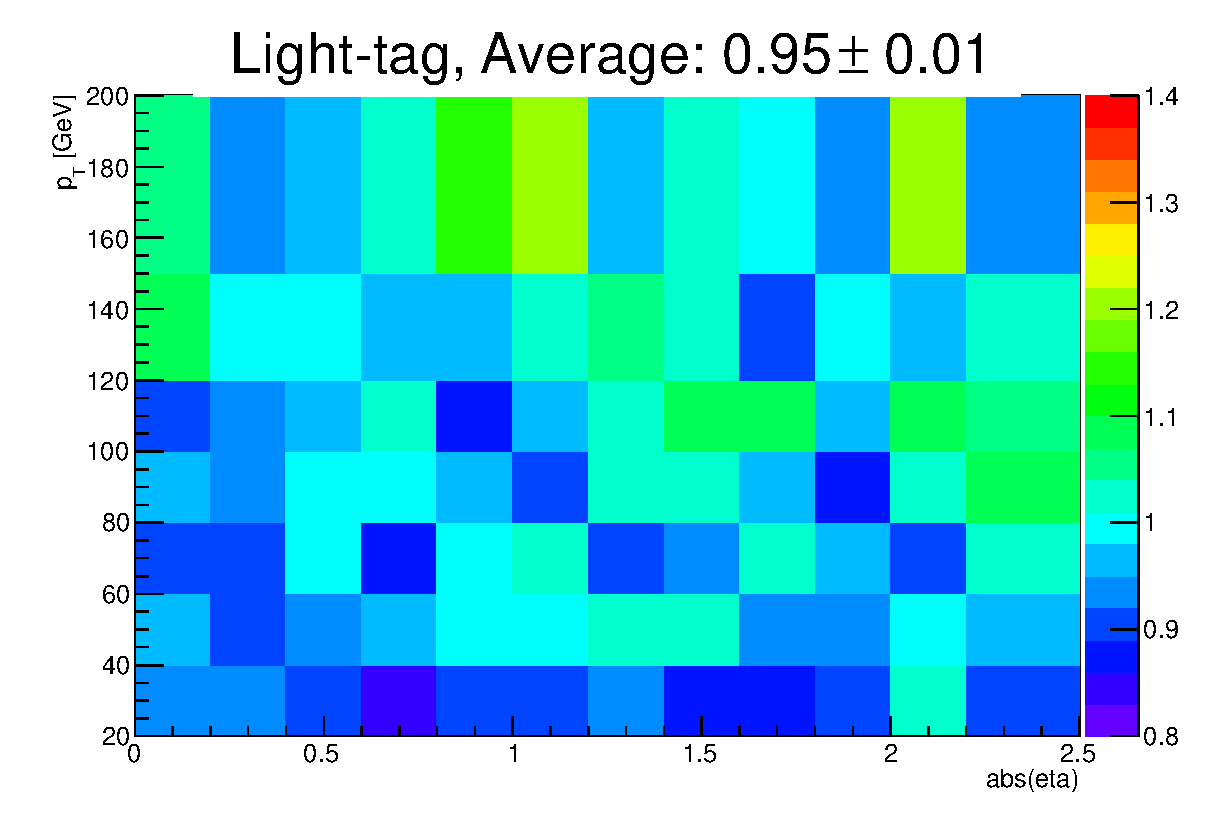
\includegraphics[width=0.45\textwidth]{appendices/figures/trf/0myclosureRebin.eps}}
	\caption{Results of the closure test using efficiency from the official calibration file (left column) and the private efficiency map (right column). The test is split in the different jet flavours: $b$-jets (top), $c$-jets (middle) and light jets (bottom).\label{fig:closure}}
\end{center}\end{figure}

As a validation check, Figure~\ref{fig:btags} compares the spectrum
of the number of \btag ged jets distribution in the  $t\bar{t}$ Monte Carlo
sample simulated with \texttt{ALPGEN} obtained using the TRF method
and the direct \btag ging. The shapes are found to be compatible.

\begin{figure}[h!tb]\begin{center}
	\subfigure[]{\label{fig:trf4j}
    \includegraphics[width=0.32\textwidth]{appendices/figures/trf/ttbarAlpgen_HFOR_ntags_4jetex.eps}}
	\subfigure[]{\label{fig:trf5j}
    \includegraphics[width=0.32\textwidth]{appendices/figures/trf/ttbarAlpgen_HFOR_ntags_5jetex.eps}}
	\subfigure[]{\label{fig:trf6j}
    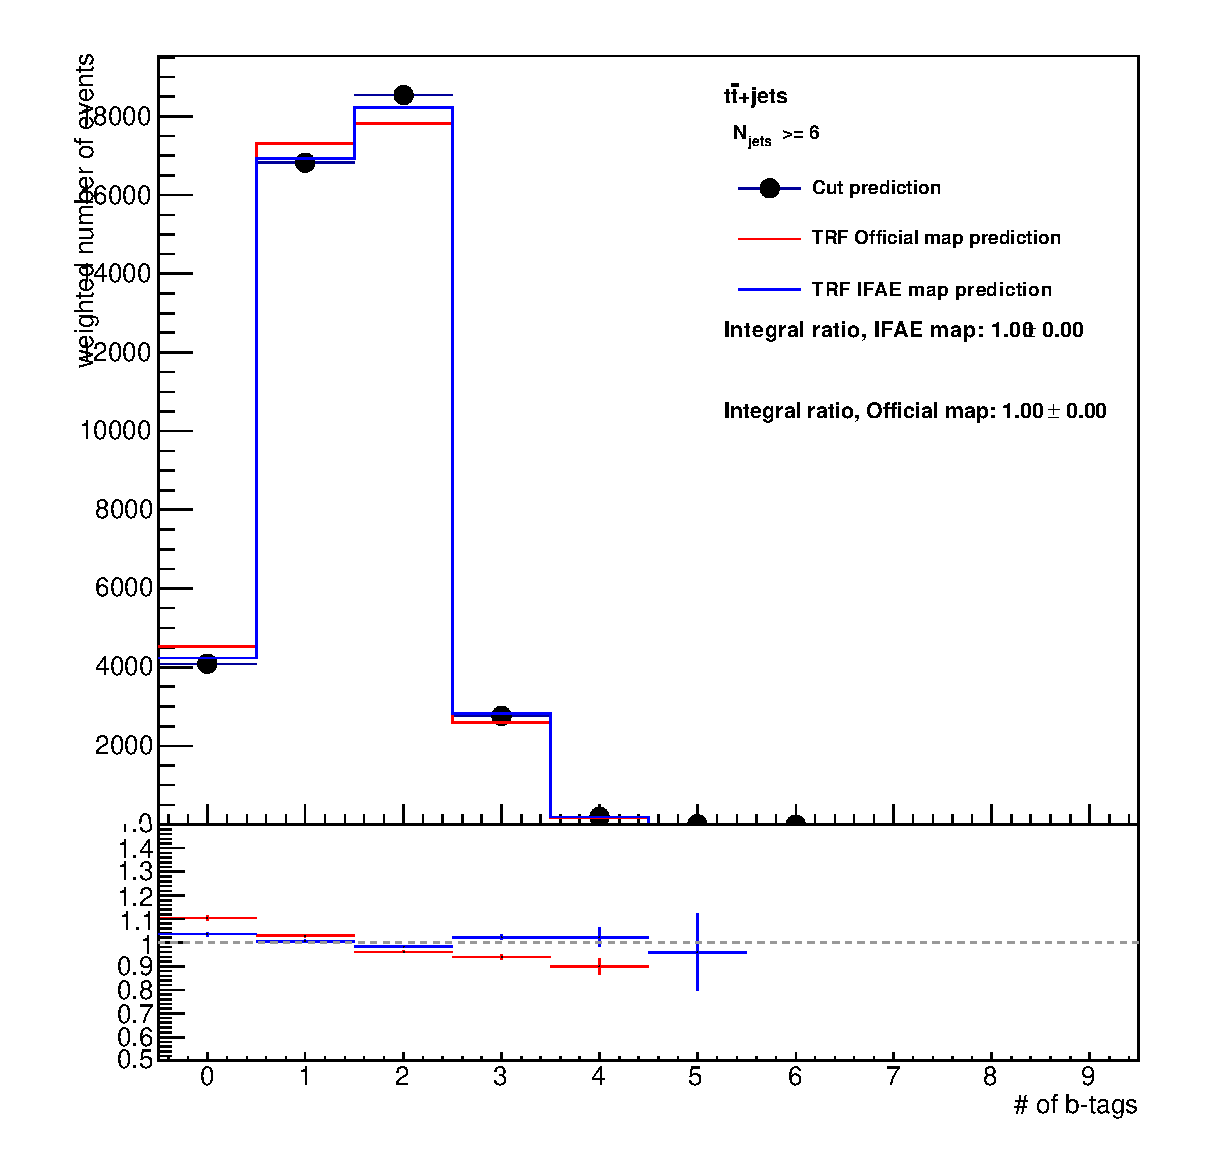
\includegraphics[width=0.32\textwidth]{appendices/figures/trf/ttbarAlpgen_HFOR_ntags_6jetin.eps}}
	\caption{Comparison of the TRF and direct $b$-tag cut prediction for the $b$-tag spectrum, in the 4 jet exclusive (a), 5 jet exclusive (b) and 6 jet inclusive (c) channels.\label{fig:btags}}
\end{center}\end{figure}


\section{TRF in the \wbx\ analysis}
%\section{TRF and \nontt\ background in the \wbx\ analysis}

As previously mentioned, the \wbx\ analysis applies the
TRF method only to Monte Carlo simulated samples of
$W/Z$+jets, single top, diboson and $t\bar{t}V$.
Table~\ref{tab:TRFvsCUT} compares the predicted yields 
at the various steps of the selection obtained
applying the TRF method and the direct cut on the
\btag ging weight for each of these simulated
processes. It can be seen that good agreement
is observed for selections where the direct \btag ging
still leaves sufficient Monte Carlo statistics,
while going tighter into the signal regions only
the TRF method returns non-zero prediction.
Also to be noted is that in all cases
the statistical uncertainty on the predicted yield is
improved by the TRF method.


\section{TRF in the \htx\ analysis}

The TRF method is used for all the Monte Carlo backgrounds in the
\htx\ analysis due to the high \btag\ multiplicity
(up to $\geq 4$) required. The validity of the method is checked by comparing 
the normalization and shape of final discriminant $H_T$ distribution
for the most relevant background, the \ttbar\ sample simulated with
\texttt{ALPGEN}, in different jet and \bjet multiplicity channels,
using the TRF method and direct \btag ging.
As it can be seen in these plots, the prediction obtained with the TRF 
method is accurate up to the statistical error.


\begin{landscape}
\begin{figure}[htb]\begin{center}
\vskip-.5cm
\hskip-1cm
\resizebox{1.5\textwidth}{!}{
	\subfigure[]{
  	\includegraphics[width=0.3\textwidth]{appendices/figures/trf/ttbarAlpgen_HFOR_htall_4jetex0btagex.eps}}
	\subfigure[]{
  	\includegraphics[width=0.3\textwidth]{appendices/figures/trf/ttbarAlpgen_HFOR_htall_4jetex1btagex.eps}}
	\subfigure[]{
  	\includegraphics[width=0.3\textwidth]{appendices/figures/trf/ttbarAlpgen_HFOR_htall_4jetex2btagex.eps}}
	\subfigure[]{
  	\includegraphics[width=0.3\textwidth]{appendices/figures/trf/ttbarAlpgen_HFOR_htall_4jetex3btagex.eps}}
	\subfigure[]{
  	\includegraphics[width=0.3\textwidth]{appendices/figures/trf/ttbarAlpgen_HFOR_htall_4jetex4btagin.eps}}}\\
\hskip-1cm
\resizebox{1.5\textwidth}{!}{
	\subfigure[]{
  	\includegraphics[width=0.3\textwidth]{appendices/figures/trf/ttbarAlpgen_HFOR_htall_5jetex0btagex.eps}}
	\subfigure[]{
  	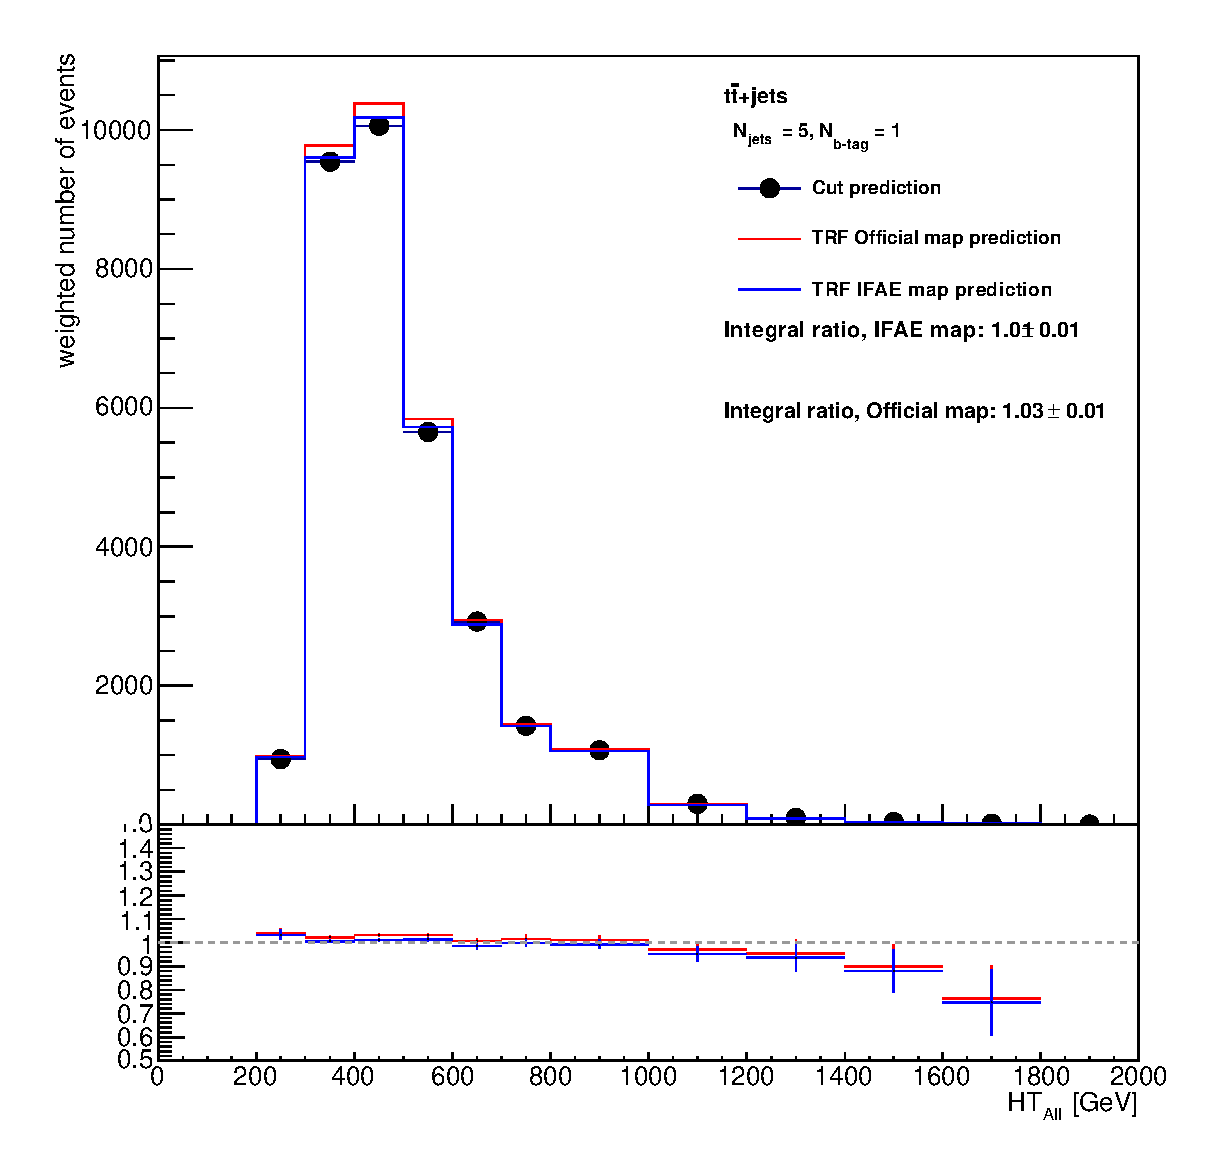
\includegraphics[width=0.3\textwidth]{appendices/figures/trf/ttbarAlpgen_HFOR_htall_5jetex1btagex.eps}}
	\subfigure[]{
  	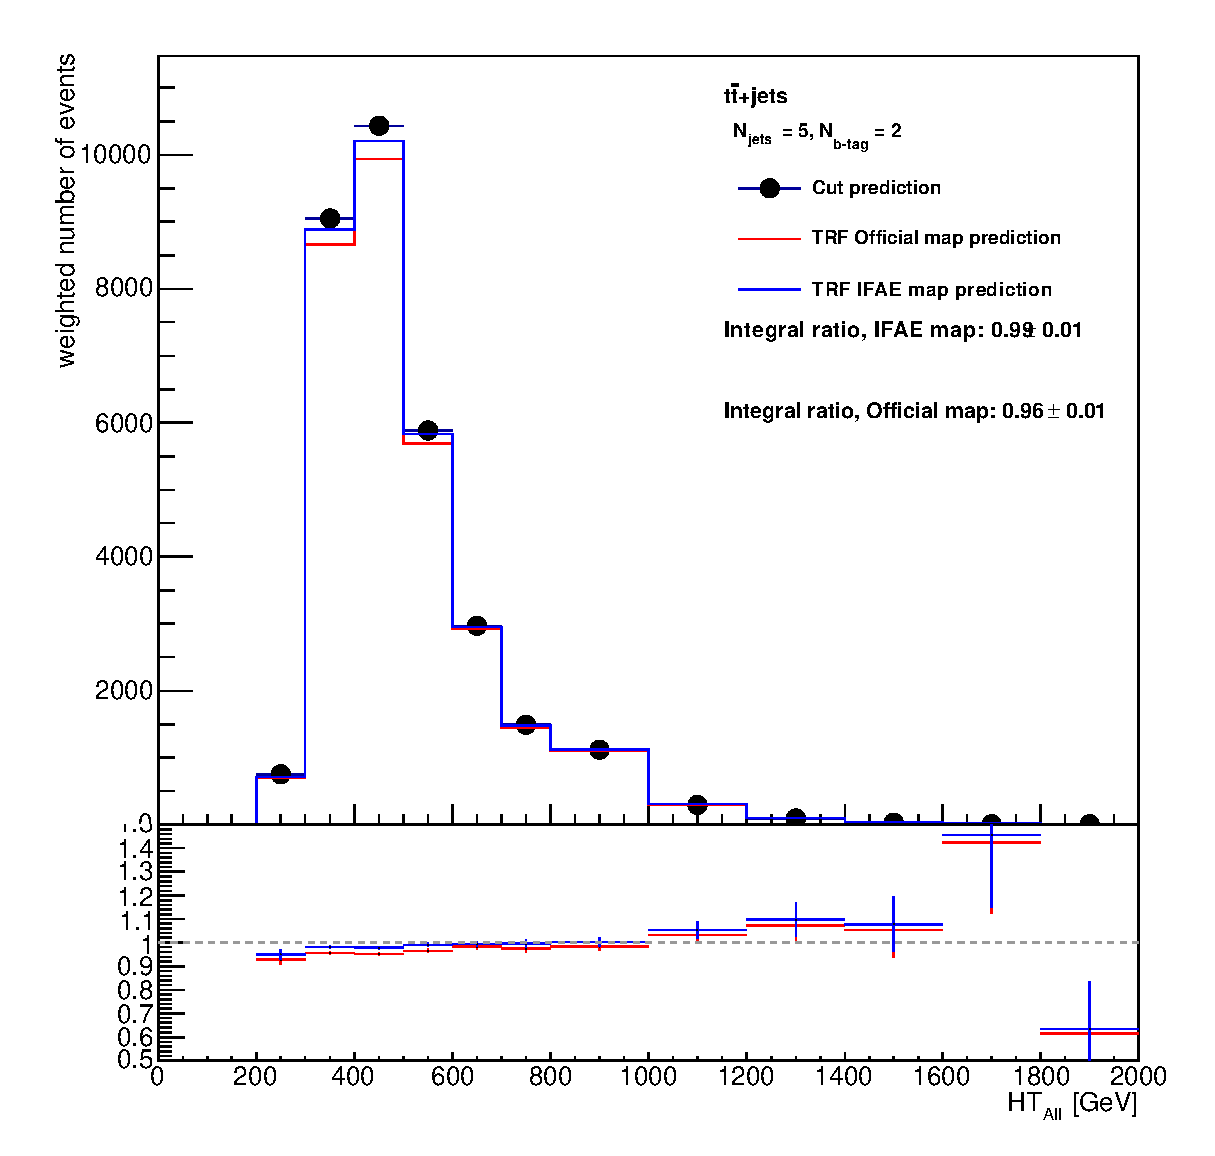
\includegraphics[width=0.3\textwidth]{appendices/figures/trf/ttbarAlpgen_HFOR_htall_5jetex2btagex.eps}}
	\subfigure[]{
  	\includegraphics[width=0.3\textwidth]{appendices/figures/trf/ttbarAlpgen_HFOR_htall_5jetex3btagex.eps}}
	\subfigure[]{
  	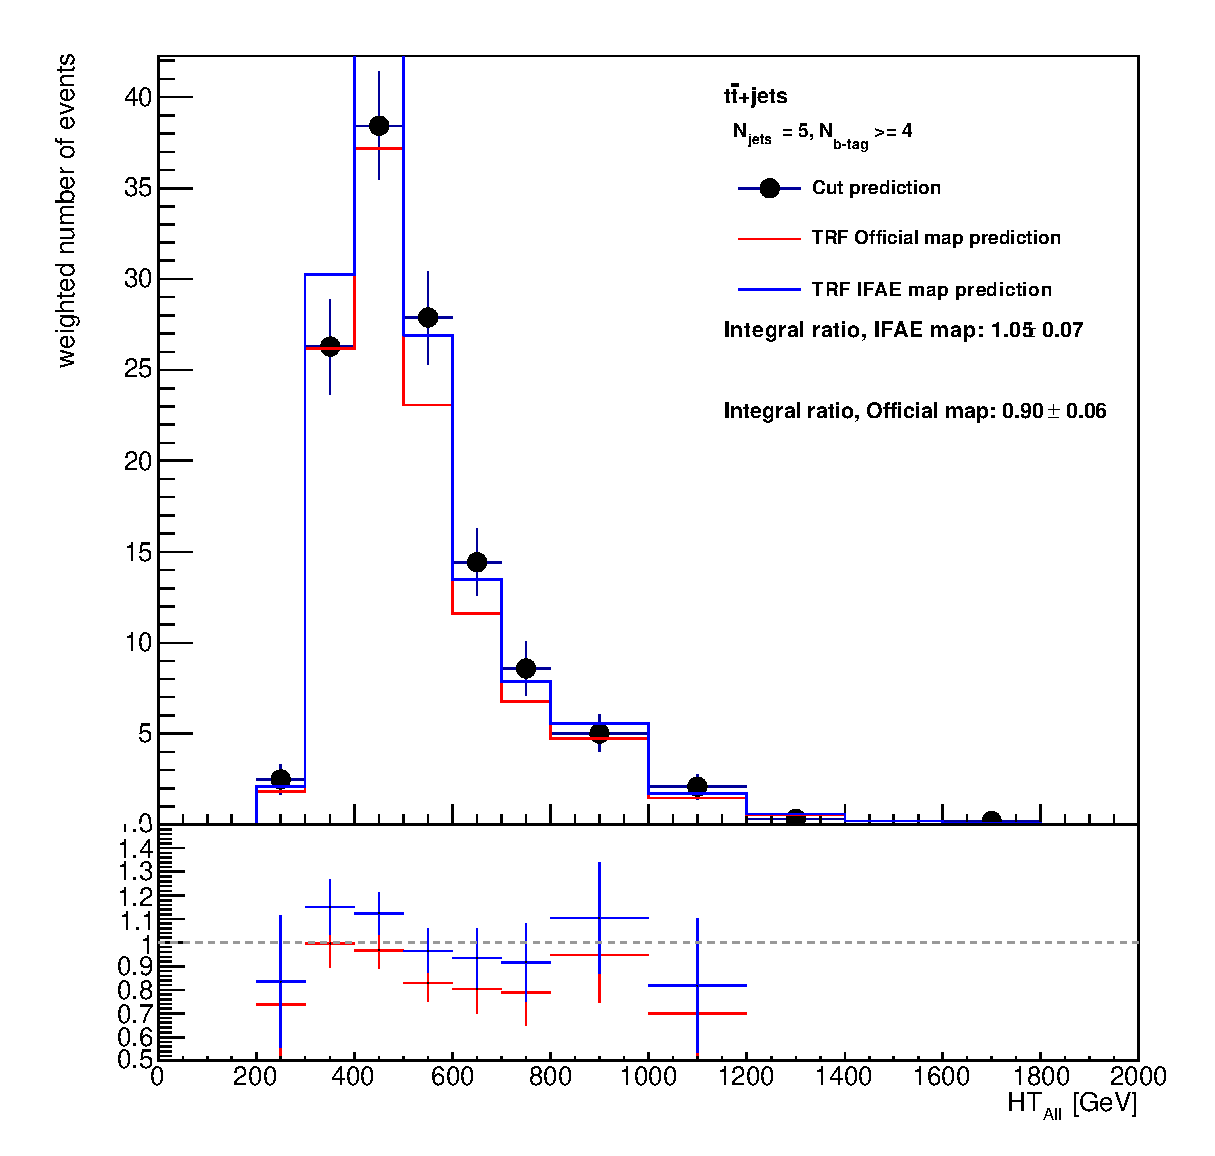
\includegraphics[width=0.3\textwidth]{appendices/figures/trf/ttbarAlpgen_HFOR_htall_5jetex4btagin.eps}}
}\\
\hskip-1cm
\resizebox{1.5\textwidth}{!}{
	\subfigure[]{
  	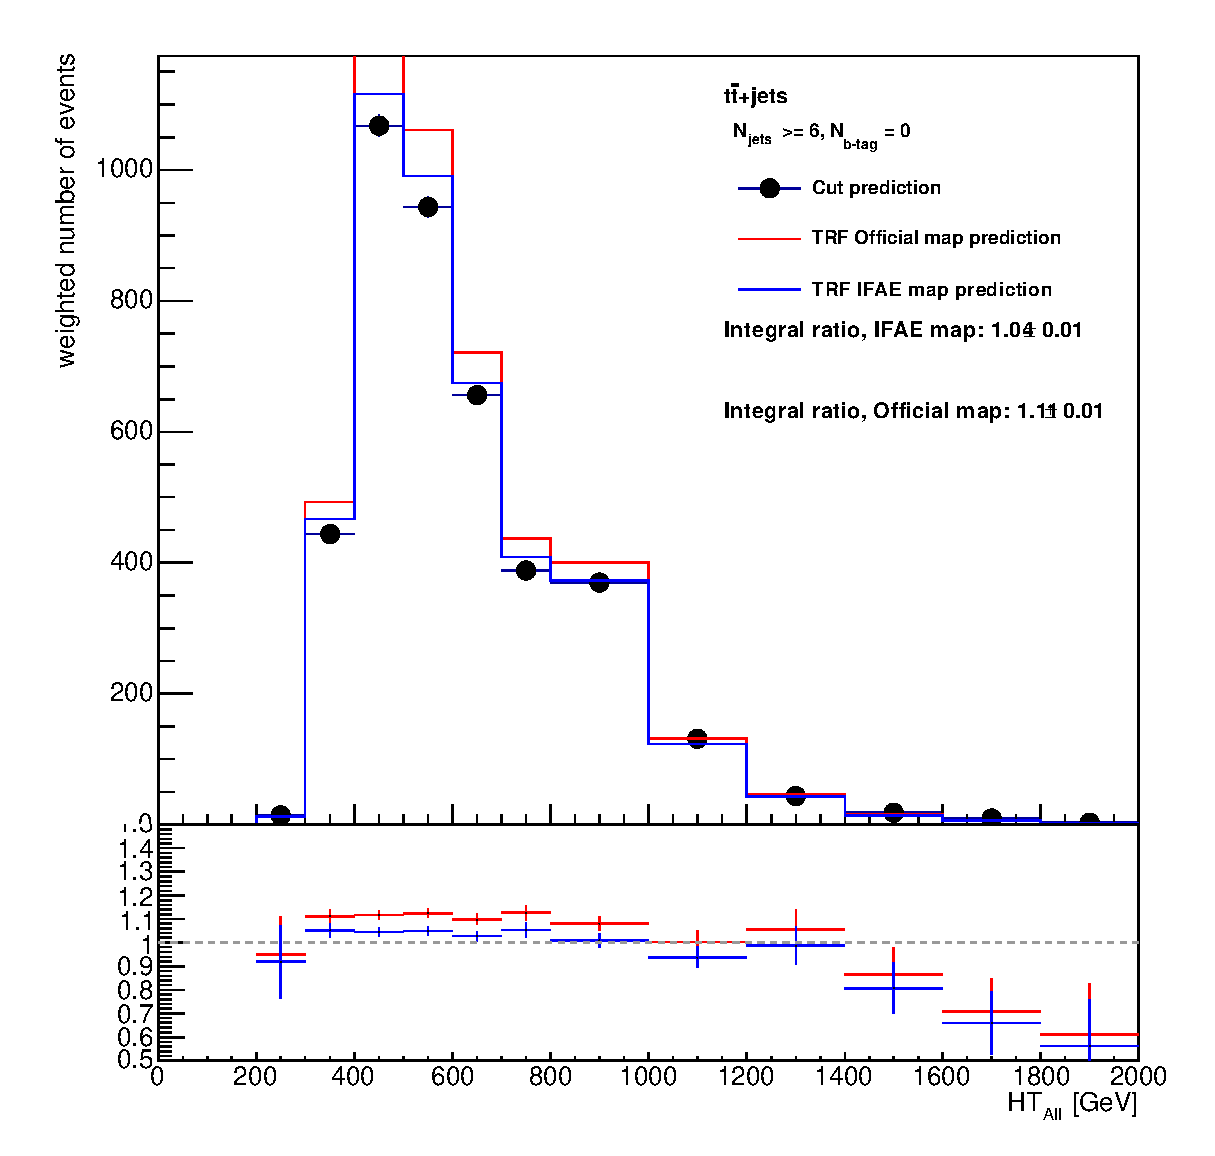
\includegraphics[width=0.3\textwidth]{appendices/figures/trf/ttbarAlpgen_HFOR_htall_6jetin0btagex.eps}}
	\subfigure[]{
  	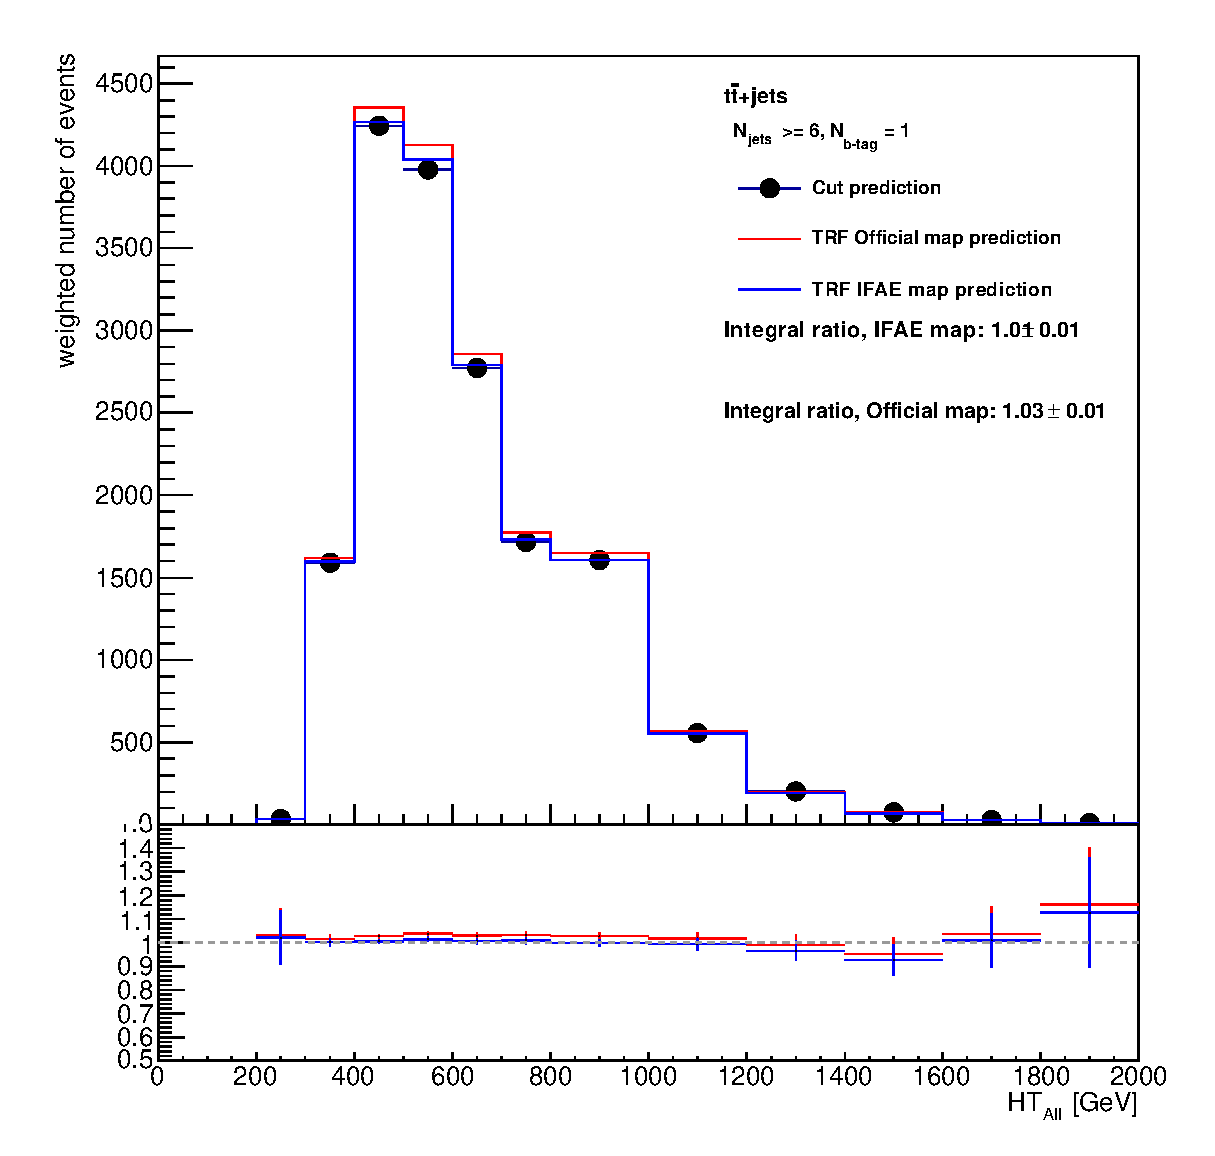
\includegraphics[width=0.3\textwidth]{appendices/figures/trf/ttbarAlpgen_HFOR_htall_6jetin1btagex.eps}}
	\subfigure[]{
  	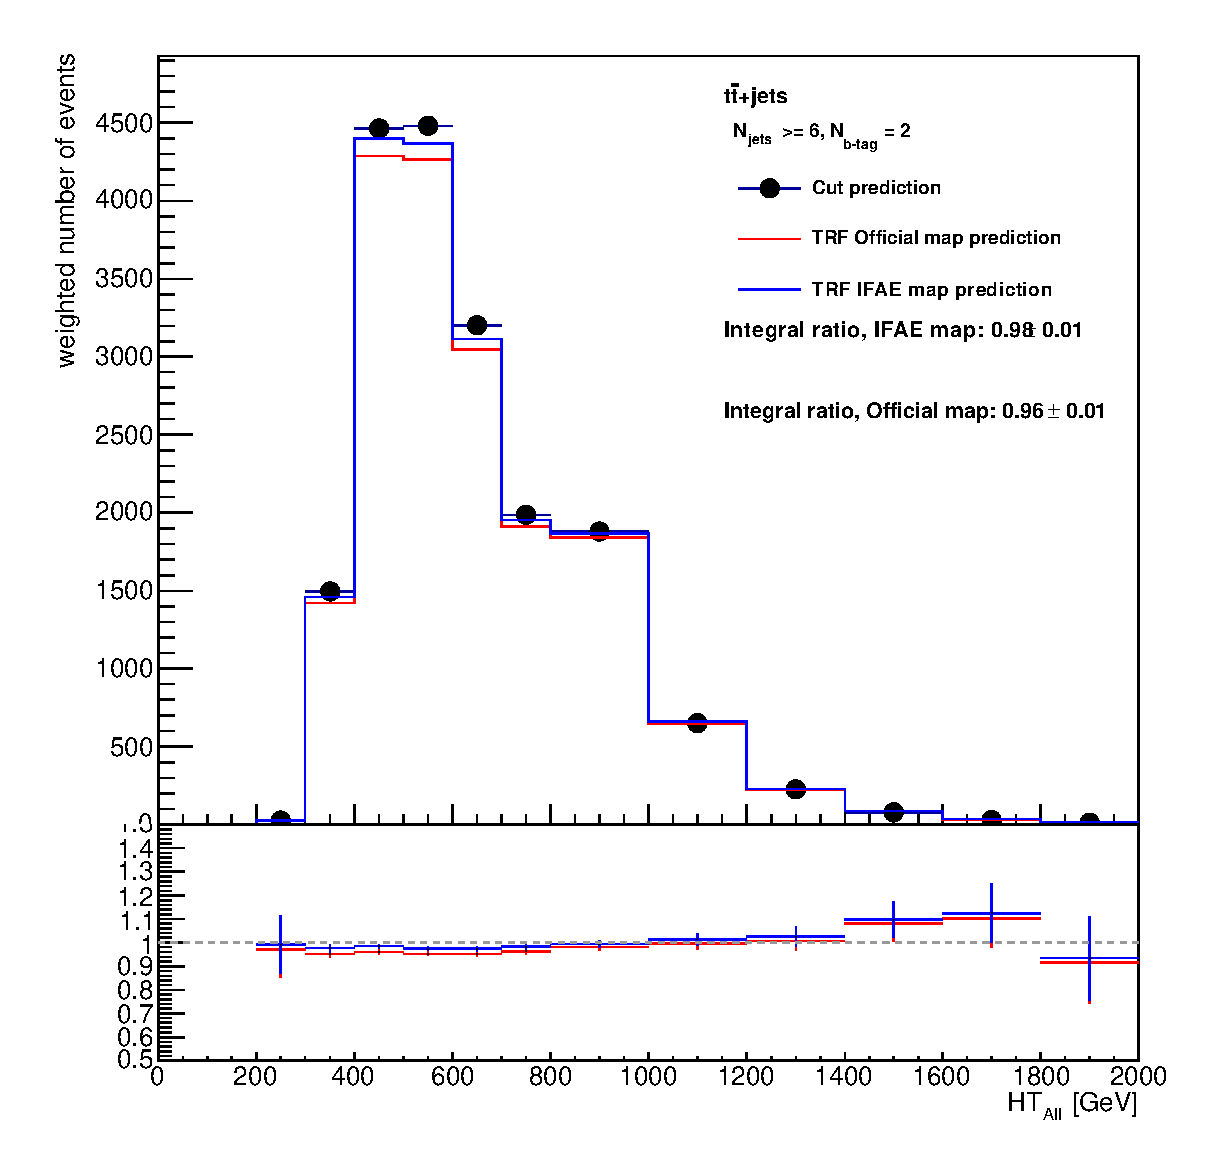
\includegraphics[width=0.3\textwidth]{appendices/figures/trf/ttbarAlpgen_HFOR_htall_6jetin2btagex.eps}}
	\subfigure[]{
  	\includegraphics[width=0.3\textwidth]{appendices/figures/trf/ttbarAlpgen_HFOR_htall_6jetin3btagex.eps}}
	\subfigure[]{
  	\includegraphics[width=0.3\textwidth]{appendices/figures/trf/ttbarAlpgen_HFOR_htall_6jetin4btagin.eps}}
}
	\caption{Comparison of the TRF and $b$-tag cut prediction for the $HT_{all}$ distribution in the (a--e) 4 jet exclusive, (f--j) 5 jet exclusive and (k--o) 6 jet inclusive channels, for different $b$-tagging multiplicities (from left to right, 0, 1, 2, 3 exclusive and 4 inclusive) for the $t\bar{t}$ \texttt{ALPGEN} sample. }
  \label{fig:validate_ttbar_ht}
\end{center}\end{figure}
\end{landscape}

%%%%%%%%%%%%%%%
\begin{table}\small
\begin{center}
\begin{tabular}{lcccc} \toprule
  & \multicolumn{2}{c}{TRF} & \multicolumn{2}{c}{Direct tagging}\\
  & Entries & Predicted yield & Entries & Predicted yield  \\
\midrule
\multicolumn{5}{c}{$W$+jets} \\
\midrule
Preselection            & 66381  & 37679.2 	$\pm$ 	324.0 	 & 8880  & 37317.3 	$\pm$ 	527.8 	\\
$\geq 1~W$              & 1321  & 723.2 	$\pm$ 	40.3 	 & 185  & 713.9 	$\pm$ 	66.7 	\\
$H_T>800~$GeV           & 520  & 314.0 	        $\pm$ 	27.4 	 & 84  & 308.0 	        $\pm$ 	41.7 	\\
$p_T(b_1) > 160~$GeV    & 262  & 146.9 	        $\pm$ 	17.8 	 & 44  & 155.3 	        $\pm$ 	30.5 	\\
$p_T(b_2) >80~$GeV      & 63  & 46.9 	        $\pm$ 	11.5 	 & 11  & 39.9 	        $\pm$ 	13.8 	\\
$\Delta R(l,\nu)<1.2$   & 28  & 16.3 	        $\pm$ 	6.0 	 & 5  & 14.7 	        $\pm$ 	7.2 	\\
min$\Delta R(l,b)>1.4$  & 15  & 6.3 	        $\pm$ 	2.8 	 & 2  & 5.2 	        $\pm$ 	4.0 	\\
min$\Delta R(W,b)>1.4$  & 9  & 5.5 	        $\pm$ 	2.8 	 & 1  & 3.7 	        $\pm$ 	3.7 	\\
\midrule
\multicolumn{5}{c}{$Z$+jets} \\
\midrule 
Preselection            & 19500  & 6054.4 	$\pm$ 	84.3 	 & 4573  & 6015.1 	$\pm$ 	147.7 	\\
$\geq 1~W$              & 331  & 133.9 	        $\pm$ 	14.2 	 & 87  & 125.9 	        $\pm$ 	19.0 	\\
$H_T>800~$GeV           & 130  & 47.8 	        $\pm$ 	8.7 	 & 32  & 49.4 	        $\pm$ 	12.2 	\\
$p_T(b_1) > 160~$GeV    & 74  & 25.2 	        $\pm$ 	6.7 	 & 19  & 29.8 	        $\pm$ 	10.2 	\\
$p_T(b_2) >80~$GeV      & 22  & 12.8 	        $\pm$ 	6.0 	 & 9  & 15.9 	        $\pm$ 	7.4 	\\
$\Delta R(l,\nu)<1.2$   & 5  & 1.1 	        $\pm$ 	0.6 	 & 1  & 0.8 	        $\pm$ 	0.8 	\\
min$\Delta R(l,b)>1.4$  & 2  & 0.2 	        $\pm$ 	0.2 	 & 0  & 0.0 	        $\pm$ 	0.0 	\\
min$\Delta R(W,b)>1.4$  & 2  & 0.2 	        $\pm$ 	0.2 	 & 0  & 0.0 	        $\pm$ 	0.0 	\\
\midrule
\multicolumn{5}{c}{Dibosons} \\
\midrule 
Preselection            & 18629  & 555.5 	$\pm$ 	7.0 	 & 3532  & 552.2 	$\pm$ 	11.4 	\\
$\geq 1~W$              & 336  & 10.9 	        $\pm$ 	1.1 	 & 50  & 8.6 	        $\pm$ 	1.4 	\\
$H_T>800~$GeV           & 85  & 2.9 	        $\pm$ 	0.6 	 & 14  & 2.4 	        $\pm$ 	0.7 	\\
$p_T(b_1) > 160~$GeV    & 32  & 0.9 	        $\pm$ 	0.3 	 & 4  & 0.5 	        $\pm$ 	0.3 	\\
$p_T(b_2) >80~$GeV      & 14  & 0.5 	        $\pm$ 	0.2 	 & 2  & 0.3 	        $\pm$ 	0.2 	\\
$\Delta R(l,\nu)<1.2$   & 9  & 0.2 	        $\pm$ 	0.1 	 & 1  & 0.1 	        $\pm$ 	0.1 	\\
min$\Delta R(l,b)>1.4$  & 8  & 0.1 	        $\pm$ 	0.1 	 & 1  & 0.1 	        $\pm$ 	0.1 	\\
min$\Delta R(W,b)>1.4$  & 4  & 0.1 	        $\pm$ 	0.0 	 & 0  & 0.0 	        $\pm$ 	0.0 	\\
\midrule
\multicolumn{5}{c}{Single top} \\
\midrule 
Preselection            & 74327  & 14670.8 	$\pm$ 	97.9 	 & 59854  & 14722.9 	$\pm$ 	107.0 	\\
$\geq 1~W$              & 2799  & 469.9 	$\pm$ 	14.1 	 & 2349  & 468.0 	$\pm$ 	14.9 	\\
$H_T>800~$GeV           & 986  & 164.7 	        $\pm$ 	7.9 	 & 826  & 162.8 	$\pm$ 	8.4 	\\
$p_T(b_1) > 160~$GeV    & 624  & 105.2 	        $\pm$ 	6.4 	 & 539  & 107.6 	$\pm$ 	6.9 	\\
$p_T(b_2) >80~$GeV      & 292  & 51.6 	        $\pm$ 	4.4 	 & 263  & 53.8 	        $\pm$ 	4.7 	\\
$\Delta R(l,\nu)<1.2$   & 165  & 30.2 	        $\pm$ 	3.6 	 & 147  & 30.4 	        $\pm$ 	3.7 	\\
min$\Delta R(l,b)>1.4$  & 61  & 14.0 	        $\pm$ 	2.4 	 & 55  & 14.0 	        $\pm$ 	2.4 	\\
min$\Delta R(W,b)>1.4$  & 21  & 4.4 	        $\pm$ 	1.3 	 & 19  & 4.8 	        $\pm$ 	1.4 	\\
\midrule
\multicolumn{5}{c}{$t\bar{t}V$} \\
\midrule 
Preselection            & 171489  & 706.1 	$\pm$ 	2.1 	 & 142296  & 709.0 	$\pm$ 	2.3 	\\
$\geq 1~W$              & 19492  & 78.6 	$\pm$ 	0.7 	 & 15862  & 78.3 	$\pm$ 	0.8 	\\
$H_T>800~$GeV           & 8516  & 34.2 	        $\pm$ 	0.5 	 & 6963  & 34.2 	$\pm$ 	0.5 	\\
$p_T(b_1) > 160~$GeV    & 4419  & 17.9 	        $\pm$ 	0.3 	 & 3657  & 18.0 	$\pm$ 	0.4 	\\
$p_T(b_2) >80~$GeV      & 2267  & 9.3        	$\pm$ 	0.2 	 & 1912  & 9.5 	        $\pm$ 	0.3 	\\
$\Delta R(l,\nu)<1.2$   & 1227  & 5.1 	        $\pm$ 	0.2 	 & 1029  & 5.2 	        $\pm$ 	0.2 	\\
min$\Delta R(l,b)>1.4$  & 321  & 1.3 	        $\pm$ 	0.1 	 & 265  & 1.4 	        $\pm$ 	0.1 	\\
min$\Delta R(W,b)>1.4$  & 138  & 0.5 	        $\pm$ 	0.1 	 & 104  & 0.6 	        $\pm$ 	0.1 	\\
\bottomrule
\end{tabular}
    
\caption{Comparison of expected yields between TRF and direct tagging as a function of cuts applied from the preselection level up to the \tight\ selection.\label{tab:TRFvsCUT}}
\end{center}
\end{table}
%%%%%%%%%%%%%%%
%%%called in event reco ch.4

\clearpage{\pagestyle{empty}\cleardoublepage}

\clearpage{\pagestyle{empty}\cleardoublepage}

\chapter{Multi-jet background estimation in the single muon plus jets channel}\label{app:qcdmm}

We report in this appendix the method developed in year 2011 to better predict
the contribution from multi-jet background events in analyses with a single
muon and jets in the final state. 
For what concerns the studies presented in this appendix, data
from pp collisions at \cme\ of 7~\tev\ collected with the ATLAS
detector in 2011 are used, with a total integrated luminosity
of 689.5~\ipb. Details on the status of top analyses
using this dataset can be found in Reference~\cite{topCommonObjects2012}.
We refer to Section~\ref{sec:qcdbkg}
for the description of the general approach of the
Matrix Method and will present here the improvements we
made in the estimation by introducing a parametrization of
the $\epsilon_\mathrm{fake}$ as a function of the leption
transverse momentum and of the minimum of $\Delta R(\mu,j)$.
These parametrizations for the fake efficiencies 
are combined with the already consolidated parametrization
in terms of muon pseudorapidity, which was used before.


The idea is that an increase in leading jet $p_T$ corresponds 
to higher hadronic activity nearby the lepton, 
which results in the fact that the event will no 
longer satisfy the tight selection requirement of 
isolation $\min\Delta R(\mu,j)>0.4$. This means a lower 
$\epsilon_\mathrm{fake}$. For the same reason we expect 
the fake efficiency to be lower for muons closer to jets.
We also expect this effects to increase with the number of 
jets in the event, a dependence that should be entering
in the $\epsilon_\mathrm{fake}$ parametrization as a function
of $\min\Delta R(\mu,j)$ (see Figure~\ref{fig:etaDep} and~\ref{fig:ljptmindrDep}). 

The muons are selected as ``tight'' if they pass the standard selection 
that was used in 2011 top analyses~\cite{topCommonObjects2012} 
(\texttt{combined} muons
passing {\tt EF$\_$mu18} trigger and track quality and isolation cuts,
summarized in Table~\ref{tab:tightloosemu}), while for the ``loose'' 
selections the requirements on calorimeter and tracker isolation
(\textit{etcone30}$<4~$GeV and \textit{ptcone30}$<4~$GeV respectively) 
are dropped.

\begin{table}[htb]\centering
\begin{tabular}{lcc}
cut & loose & tight \\\midrule
track ID quality cuts & $\checkmark$ & $\checkmark$\\
\texttt{combined} muon & $\checkmark$ & $\checkmark$\\
\texttt{tight} muon & $\checkmark$ & $\checkmark$\\
min$\Delta R(\mu,j)>0.4$ & $\checkmark$ & $\checkmark$\\
$e/\mu$ overlap removal& $\checkmark$ & $\checkmark$\\
\texttt{etcone30} $<4~$GeV &  & $\checkmark$\\
\texttt{ptcone30} $<4~$GeV &  & $\checkmark$\\\bottomrule
\end{tabular}
\caption{Selection cuts for tight and loose muons. The track ID quality cuts include
 $\pt(\mu) > 20 \GeV$ and $|\eta(\mu)| < 2.5$.}\label{tab:tightloosemu}
\end{table}

$\epsilon_\mathrm{real}$ is estimated in a sample of $Z\rightarrow \mu\mu$ 
restricted to events with exactly 2 muons, one ``tight'' and one ``loose'' 
and requiring the dilepton reconstructed mass of the boson to be between 80-100~GeV. 
The control region to estimate $\epsilon_\mathrm{f}$ is chosen as 
$5$~GeV$< E^{Miss}_T<15$~GeV in order to isolate a sample enriched 
in QCD, then the event is required to have a ``loose'' muon and at 
least one jet. Since contamination from muons from $W$ and $Z$ decays 
is still present in the low $E^{Miss}_T$ region, we try to achieve 
higher purity by correcting $N^{tight}$ and $N^{loose}$ as 
\begin{eqnarray}
N^{tight}_{corr} &&=  N^{tight} - N^{tight}_{W+jets,MC} - N^{tight}_{Z+jets,MC}) - N^{tight}_{t\bar{t},MC}\\
N^{loose}_{corr} &&=  N^{loose} - N^{loose}_{W+jets,MC} - N^{loose}_{Z+jets,MC}) - N^{loose}_{t\bar{t},MC}
\end{eqnarray}

Figure~\ref{fig:etaDep}~and~\ref{fig:ljptmindrDep}  
show $\epsilon_\mathrm{r}$ as a function of muon $\eta$ 
and  $\epsilon_\mathrm{f}$ as a function of the variables 
on which we parametrize, i.e. muon $\eta$, leading jet $p_T$ 
and the minimum of $\Delta R(\mu,j)$.  The functions used don't 
have a specific physical meaning and are respectively 
\begin{equation}\label{eq:paruntagljpt}
f_{LJpT}(x) = p_0 + p_1/(x/100)^{p_2}
\end{equation} and 
\begin{equation}\label{eq:parmindr}
f_{min\Delta R}(x) = 0.5 p_0 (1+TMath::Erf( (x-p_1)/(\sqrt{2}p_2))).
\end{equation} 

If we add the requirement of having at least one tagged jet in 
the event, the efficiencies change (see Table~\ref{tab:averageeffs}). 
Efficiencies are computed in the same way as the untagged case 
but separately and requiring at least 1 \btag ged jet, where at the
time the \btag ging algorithm used was \texttt{SV0} with a weight cut 
of 5.85. While different fake efficiencies where obtained in the
parametrizations with respect to lepton $\eta$ and jet \pt, 
no significant variations were observed in the dependency on
the minimum $\Delta R(\mu,j)$ and the pre-tag efficiencies are 
used in that case to exploit the higher statistics, like it's done for 
$\epsilon_\mathrm{r}$ where again the \btag ged events show 
no significant differences and more statistics 
for the estimation is available.

\begin{figure}\centering
\includegraphics[width=.45\textwidth]{appendices/figures/mujets_mmB/fit_h_lep_eta_muon_real_untagged}\includegraphics[width=.45\textwidth]{appendices/figures/mujets_mmB/fit_h_lep_eta_muon_fake_untagged}
\caption{Lepton $\eta$ dependency of $\epsilon_\mathrm{r}$ (left plot) and $\epsilon_\mathrm{f}$ (right plot).}\label{fig:etaDep}
\end{figure} \begin{figure}\centering
\includegraphics[width=.45\textwidth]{appendices/figures/mujets_mmB/fit_h_lep_LJpT_rb_muon_fake_untagged}\includegraphics[width=.45\textwidth]{appendices/figures/mujets_mmB/fit_h_lep_minDR_muon_fake_untagged}
\caption{Parametrization of $\epsilon_\mathrm{f}$ as a function of the leading jet $p_T$ (left plot) and of the minimum $\Delta R$ between muon and jets (right plot). }\label{fig:ljptmindrDep}
\end{figure} 

\begin{table}\centering
\begin{tabular}{l c c }
\toprule
 & $\epsilon_\mathrm{f}$ &  $\epsilon_\mathrm{r}$  \\\midrule
untagged & $0.4178 \pm 0.0006 $ & $ 0.9805 \pm 0.0003 $ \\
tagged   & $0.353  \pm 0.002 $ & $ 0.973 \pm 0.006 $ \\\bottomrule
\end{tabular}\caption{Average values for $\epsilon_\mathrm{f}$ and  $\epsilon_\mathrm{r}$ in untagged and tagged channels. Error is only statistical.}\label{tab:averageeffs}
\end{table} 

The two $\epsilon_\mathrm{f}$ dependencies on  
leading jet $p_T$ and minimum $\Delta R$ between muon and 
jets  are then combined together to obtain a weight for the value of 
the fake efficiency at a given $\eta$:
\begin{equation}
\epsilon_\mathrm{f} = \epsilon_\mathrm{f}(\eta) \dfrac{f_{min\Delta R}(min\Delta R)}{<\epsilon_\mathrm{f}^{min\Delta R}>}\dfrac{f_{LJpT}(LJpT)}{<\epsilon_\mathrm{f}^{LJpT}>}.
\end{equation}

Figure~\ref{fig:datamc1} shows the agreement between data and Monte Carlo 
backgrounds 
when the QCD multi-jet backgorund estimated with this Matrix Method 
is considered. Here the events satisfy the full standard 
selection for top analyses~\cite{topCommonObjects2012} with 
exactly 1 jet before and after applying the triangular cut 
$E_T^{Miss} + m_T(W)>60~$GeV, which basically kills QCD multi-jet
contributions, and no btagging information is 
required. Adding the tagging selection leads to the comparison 
plots of Figure~\ref{fig:datamc2} where the full selection (with 
and without the triangular cut) leave exactly 2 jets of which at 
least one has been tagged as a \bjet. The variables $p_T(\mu)$, 
$E_T^{Miss}$ and $m_T(W)$ are chosen to illustrate the QCD multi-jet 
background prediction since it is known that here the QCD multi-jet will peak at 
low values. 
%In the Appendix~\ref{app:extradatamc} more plots 
%for other jet multiplicities can be found.



\begin{figure}[htb]\centering
\includegraphics[width=.3\textwidth]{{appendices/figures/mujets_mmB/hpresel_muon_pT_0btagin5.85SV0_1jetex25_MUON_MET20_HTAll0}.eps}
\includegraphics[width=.3\textwidth]{{appendices/figures/mujets_mmB/hpresel_missingET_missET_0btagin5.85SV0_1jetex25_MUON_MET20_HTAll0}.eps}
\includegraphics[width=.3\textwidth]{{appendices/figures/mujets_mmB/hmuon_Wlep_MassT_0btagin5.85SV0_1jetex25_MUON_MET20_HTAll0}.eps}\\
\includegraphics[width=.3\textwidth]{{appendices/figures/mujets_mmB/hpresel_muon_pT_0btagin5.85SV0_1jetex25_MUON_MET20_MTW_MET60_-1}.eps}
\includegraphics[width=.3\textwidth]{{appendices/figures/mujets_mmB/hpresel_missingET_missET_0btagin5.85SV0_1jetex25_MUON_MET20_MTW_MET60_-1}.eps}
\includegraphics[width=.3\textwidth]{{appendices/figures/mujets_mmB/hmuon_Wlep_MassT_0btagin5.85SV0_1jetex25_MUON_MET20_MTW_MET60_-1}.eps}
\caption{Comparison plots between data and backgrounds for the muon transverse momentum (left column), missing transverse energy (central column) and the transverse mass of the $W$ (right column). The full event selection of 1 jet exclusive with no btagging information is used without and with the triangular cut (top and bottom respectively).}\label{fig:datamc1}
\end{figure} 
\begin{figure}[htb]\centering
\includegraphics[width=.3\textwidth]{{appendices/figures/mujets_mmB/hpresel_muon_pT_1btagin5.85SV0_2jetex2525_MUON_MET20_HTAll0}.eps}
\includegraphics[width=.3\textwidth]{{appendices/figures/mujets_mmB/hpresel_missingET_missET_1btagin5.85SV0_2jetex2525_MUON_MET20_HTAll0}.eps}
\includegraphics[width=.3\textwidth]{{appendices/figures/mujets_mmB/hmuon_Wlep_MassT_1btagin5.85SV0_2jetex2525_MUON_MET20_HTAll0}.eps}\\
\includegraphics[width=.3\textwidth]{{appendices/figures/mujets_mmB/hpresel_muon_pT_1btagin5.85SV0_2jetex2525_MUON_MET20_MTW_MET60_-1}.eps}
\includegraphics[width=.3\textwidth]{{appendices/figures/mujets_mmB/hpresel_missingET_missET_1btagin5.85SV0_2jetex2525_MUON_MET20_MTW_MET60_-1}.eps}
\includegraphics[width=.3\textwidth]{{appendices/figures/mujets_mmB/hmuon_Wlep_MassT_1btagin5.85SV0_2jetex2525_MUON_MET20_MTW_MET60_-1}.eps}
\caption{Comparison plots between data and backgrounds for the muon transverse momentum (left column), missing transverse energy (central column) and the transverse mass of the $W$ (right column). The full event selection of 2 jet exclusive with at least 1 btagged jet is used without and with the triangular cut (top and bottom respectively).}\label{fig:datamc2}
\end{figure} 


The two plots in Figure~\ref{fig:jetmultiplicity} show the 
total amount of events for data and backgrounds in the pre-tagged 
and \btag ged channels in different jet multiplicity bins. 
The numerical values for the QCD estimate are reported in 
Table~\ref{tab:yieldsuntagged} and Table~\ref{tab:yieldstagged} 
for the pre-tagged and \btag ged case respectively.

\begin{figure}[htb]\centering
\includegraphics[width=.45\textwidth]{{appendices/figures/mujets_mmB/nJets_MUON_0btagin5.85SV0_MET20_MTW_MET60_-1}.eps}
\includegraphics[width=.45\textwidth]{{appendices/figures/mujets_mmB/nJets_MUON_1btagin5.85SV0_MET20_MTW_MET60_-1}.eps}
\caption{Yields plots for data and backgrounds requiring full event selection (left plot) and full event selection plus at least one btagged jet (right plot) in jet multiplicity bins.}\label{fig:jetmultiplicity}
\end{figure}

\begin{table}[h!tb]\centering
\resizebox{1.\textwidth}{!}{
\begin{tabular}{l c c c c}
\toprule
 & = 1 jet & = 2 jets & = 3 jets & $\ge$ 4 jets \\
\midrule
$t\bar{t}$& 304.33 $\pm$  7.41 &1320.55 $\pm$  15.50 &2709.63 $\pm$  22.13 &4702.33 $\pm$29.49\\
QCD & 24803.36 $\pm$  153.57 &10511.66 $\pm$  87.94 &2942.08 $\pm$  43.72 &1049.85 $\pm$25.02\\
W+jets& 385242.06 $\pm$  1129.55 &98826.98 $\pm$  373.93 &23614.51 $\pm$  154.62 &7419.73 $\pm$81.07\\
Z+jets& 17257.90 $\pm$  63.81 &5478.57 $\pm$  35.64 &1553.30 $\pm$  18.79 &592.78 $\pm$11.28\\
Single top& 1002.70 $\pm$  10.77 &1126.85 $\pm$  10.55 &578.51 $\pm$  6.47 &285.44 $\pm$4.15\\
\midrule
Total prediction & 428610.34 $\pm$1141.80 & 117264.61 $\pm$386.23 & 31398.04 $\pm$163.41 & 14050.14 $\pm$90.62 \\
Data& 437526 &112984 &29135 &12779\\
\bottomrule
\end{tabular}}
\caption{Yields table for the data and background samples for different jet multiplicities in the untagged full event selection.}\label{tab:yieldsuntagged}
\end{table} 


\begin{table}[h!tb]\centering
\resizebox{1.\textwidth}{!}{
\begin{tabular}{l c c c c}
\toprule
 & = 1 jet & = 2 jets & = 3 jets & $\ge$ 4 jets \\
\midrule
$t\bar{t}$& 108.35 $\pm$  4.22 &689.18 $\pm$  10.58 &1659.28 $\pm$  16.48 &3185.88 $\pm$23.19\\
QCD & 1449.22 $\pm$  29.45 &1109.84 $\pm$  24.17 &420.08 $\pm$  14.44 &211.11 $\pm$10.35\\
W+jets& 4392.92 $\pm$  77.83 &3016.70 $\pm$  56.17 &1280.12 $\pm$  38.41 &612.50 $\pm$26.04\\
Z+jets& 104.68 $\pm$  4.76 &94.69 $\pm$  4.56 &52.10 $\pm$  3.32 &28.77 $\pm$2.44\\
Single top& 359.78 $\pm$  6.16 &522.23 $\pm$  6.80 &307.53 $\pm$  4.50 &159.42 $\pm$2.96\\
\midrule
Total prediction & 6414.95 $\pm$83.69 & 5432.64 $\pm$62.60 & 3719.11 $\pm$44.57 & 4197.68 $\pm$36.58 \\
Data& 7243 &5634 &3876 &4406\\
\bottomrule
\end{tabular}}
\caption{Yields table for the data and background samples for different jet multiplicities in the tagged full event selection (at least one bjet).}\label{tab:yieldstagged}
\end{table} 


An estimation of the systematic uncertainties on the QCD multi-jet background
as derived in this Matrix Method
can be evaluated considering the following sources:
\begin{enumerate}
 \item statistical error on  $\epsilon_\mathrm{f}$ and  $\epsilon_\mathrm{r}$;
\item statistical error on the QCD estimation;
\item different control regions for the estimation of fake efficiency;
\item changes in the parametrization used.
\end{enumerate} 
For the points 1 and 2, the values can be taken from what already 
shown in Table~\ref{tab:averageeffs} and 
Tables~\ref{tab:yieldsuntagged}~and~\ref{tab:yieldstagged}. For what 
concerns point 3, we compared the results obtained in control region 
$5$~GeV$< E^{Miss}_T<15$~GeV with an estimation in control region 
$ E^{Miss}_T<10$~GeV, while no studies have yet been performed about 
point 4. Table~\ref{tab:systuncertuntag}~and~\ref{tab:systuncerttag} 
summarize the systematic uncertainties for different jet multiplicity 
in the untagged and tagged channels respectively.


\begin{table}[h!tb]\centering
\begin{tabular}{l c c c c}
\toprule
 & = 1 jet & = 2 jets & = 3 jets & $\ge$ 4 jets \\
\midrule
$\varepsilon_1 $ & \multicolumn{4}{c}{ 0.1\% } \\
%QCD & 24803.36 $\pm$  153.57 &10511.66 $\pm$  87.94 &2942.08 $\pm$  43.72 &1049.85 $\pm$25.02\\
$\varepsilon_2 $ &  0.6\% & 0.8\% & 1.5\% & 2.4\% \\
%$\varepsilon_3 $ &  \\
$\varepsilon_3 $ & 7.9\% &  21.2\% &   31.0\% &   41.3\% \\\bottomrule
\end{tabular}\caption{Systematic uncertainties on QCD estimation for different jet multiplicity in the untagged case.}\label{tab:systuncertuntag}
%\end{table} 
%\begin{table}[hbt]\centering
\begin{tabular}{l c c c c}
\toprule
 & = 1 jet & = 2 jets & = 3 jets & $\ge$ 4 jets \\
\midrule
$\varepsilon_1 $ & \multicolumn{4}{c}{ 0.5\% } \\
%QCD & 1449.22 $\pm$  29.45 &1109.84 $\pm$  24.17 &420.08 $\pm$  14.44 &211.11 $\pm$10.35\\
$\varepsilon_2 $ &  2.0\% & 2.2\% & 3.4\% & 4.9\% \\
%$\varepsilon_3 $ &  \\
$\varepsilon_3 $ & 6.4\% &  18.5\% &   26.5\% &   32.4\% \\\bottomrule
\end{tabular}\caption{Systematic uncertainties on QCD estimation for different jet multiplicity in the tagged case.}\label{tab:systuncerttag}
\end{table} 




%\begin{figure}[htb]\begin{center}
%	\subfigure[]{\label{fig:MMmindr}
%        \begin{overpic}[width=0.47\textwidth]{vlq_analysis/figures/qcd_eff/fit_h_lep_minDR_muon_fake}
%        \put(0,50){\small \rotatebox{90}{$\varepsilon_{\rm fake}$}}
%        \put(70,0){\footnotesize min$\Delta R(\mu,j)$}
%        \end{overpic}
%        }
%  	%\includegraphics[width=0.47\textwidth]{vlq_analysis/figures/qcd_eff/fit_h_lep_minDR_muon_fake}}
%	\subfigure[]{\label{fig:MMmindr}
%        \begin{overpic}[width=0.47\textwidth]{vlq_analysis/figures/qcd_eff/fit_h_lep_LJpT_rb_muon_fake}
%        \put(0,50){\small \rotatebox{90}{$\varepsilon_{\rm fake}$}}
%        \put(60,0){\footnotesize leading jet $p_T$ [GeV]}
%        \end{overpic}
%        }
%  	%\includegraphics[width=0.47\textwidth]{vlq_analysis/figures/qcd_eff/fit_h_lep_LJpT_rb_muon_fake}}
%	\caption{}
%\end{center}\end{figure}

%%%called in vlq strat ch.5

\clearpage{\pagestyle{empty}\cleardoublepage}

\clearpage{\pagestyle{empty}\cleardoublepage}

\chapter{Data to Monte Carlo comparison in the preselection region}
\label{app:datamcpresel}

\section{Data to Monte Carlo comparison vetoing \bjet s}
\label{app:datamc0tagex}

\subsection{Electron channel}

\begin{figure}[htb]\begin{center}
	\subfigure[]{
  	\includegraphics[width=0.32\textwidth]{vlq_analysis/figures/THESIS_c5_presel_noortho_noyields/ELE/4jetin/0btagex/Njets25_ELE_4jetin0btagex_NOMINAL}}
	\subfigure[]{
  	\includegraphics[width=0.32\textwidth]{vlq_analysis/figures/THESIS_c5_presel_noortho_noyields/ELE/4jetin/0btagex/JetPt1_ELE_4jetin0btagex_NOMINAL}}
	\subfigure[]{
  	\includegraphics[width=0.32\textwidth]{vlq_analysis/figures/THESIS_c5_presel_noortho_noyields/ELE/4jetin/0btagex/JetEta1_ELE_4jetin0btagex_NOMINAL}}\\
	\subfigure[]{
  	\includegraphics[width=0.32\textwidth]{vlq_analysis/figures/THESIS_c5_presel_noortho_noyields/ELE/4jetin/0btagex/MET_ELE_4jetin0btagex_NOMINAL}}
	\subfigure[]{
  	\includegraphics[width=0.32\textwidth]{vlq_analysis/figures/THESIS_c5_presel_noortho_noyields/ELE/4jetin/0btagex/LepPt_ELE_4jetin0btagex_NOMINAL}}
	\subfigure[]{
  	\includegraphics[width=0.32\textwidth]{vlq_analysis/figures/THESIS_c5_presel_noortho_noyields/ELE/4jetin/0btagex/LepEta_ELE_4jetin0btagex_NOMINAL}}\\
	\subfigure[]{
  	\includegraphics[width=0.32\textwidth]{vlq_analysis/figures/THESIS_c5_presel_noortho_noyields/ELE/4jetin/0btagex/Wlep_MassT_ELE_4jetin0btagex_NOMINAL}}
	\subfigure[]{
  	\includegraphics[width=0.32\textwidth]{vlq_analysis/figures/THESIS_c5_presel_noortho_noyields/ELE/4jetin/0btagex/HTHad_ELE_4jetin0btagex_NOMINAL}}
	\subfigure[]{
  	\includegraphics[width=0.32\textwidth]{vlq_analysis/figures/THESIS_c5_presel_noortho_noyields/ELE/4jetin/0btagex/HTAll_ELE_4jetin0btagex_NOMINAL}}
	\caption{ \label{fig:ELE_4jetin0btagex}}
\end{center}\end{figure}

\subsection{Muon channel}


\begin{figure}[htb]\begin{center}
	\subfigure[]{
  	\includegraphics[width=0.32\textwidth]{vlq_analysis/figures/THESIS_c5_presel_noortho_noyields/MUON/4jetin/0btagex/Njets25_MUON_4jetin0btagex_NOMINAL}}
	\subfigure[]{
  	\includegraphics[width=0.32\textwidth]{vlq_analysis/figures/THESIS_c5_presel_noortho_noyields/MUON/4jetin/0btagex/JetPt1_MUON_4jetin0btagex_NOMINAL}}
	\subfigure[]{
  	\includegraphics[width=0.32\textwidth]{vlq_analysis/figures/THESIS_c5_presel_noortho_noyields/MUON/4jetin/0btagex/JetEta1_MUON_4jetin0btagex_NOMINAL}}\\
	\subfigure[]{
  	\includegraphics[width=0.32\textwidth]{vlq_analysis/figures/THESIS_c5_presel_noortho_noyields/MUON/4jetin/0btagex/MET_MUON_4jetin0btagex_NOMINAL}}
	\subfigure[]{
  	\includegraphics[width=0.32\textwidth]{vlq_analysis/figures/THESIS_c5_presel_noortho_noyields/MUON/4jetin/0btagex/LepPt_MUON_4jetin0btagex_NOMINAL}}
	\subfigure[]{
  	\includegraphics[width=0.32\textwidth]{vlq_analysis/figures/THESIS_c5_presel_noortho_noyields/MUON/4jetin/0btagex/LepEta_MUON_4jetin0btagex_NOMINAL}}\\
	\subfigure[]{
  	\includegraphics[width=0.32\textwidth]{vlq_analysis/figures/THESIS_c5_presel_noortho_noyields/MUON/4jetin/0btagex/Wlep_MassT_MUON_4jetin0btagex_NOMINAL}}
	\subfigure[]{
  	\includegraphics[width=0.32\textwidth]{vlq_analysis/figures/THESIS_c5_presel_noortho_noyields/MUON/4jetin/0btagex/HTHad_MUON_4jetin0btagex_NOMINAL}}
	\subfigure[]{
  	\includegraphics[width=0.32\textwidth]{vlq_analysis/figures/THESIS_c5_presel_noortho_noyields/MUON/4jetin/0btagex/HTAll_MUON_4jetin0btagex_NOMINAL}}
	\caption{\label{fig:MUON_4jetin0btagex}}
\end{center}\end{figure}



\subsection{Electron+Muon channel}

\begin{figure}[htb]\begin{center}
	\subfigure[]{
  	\includegraphics[width=0.32\textwidth]{vlq_analysis/figures/THESIS_c5_presel_noortho_noyields/ELEMUON/4jetin/0btagex/Njets25_ELEMUON_4jetin0btagex_NOMINAL}}
	\subfigure[]{
  	\includegraphics[width=0.32\textwidth]{vlq_analysis/figures/THESIS_c5_presel_noortho_noyields/ELEMUON/4jetin/0btagex/JetPt1_ELEMUON_4jetin0btagex_NOMINAL}}
	\subfigure[]{
  	\includegraphics[width=0.32\textwidth]{vlq_analysis/figures/THESIS_c5_presel_noortho_noyields/ELEMUON/4jetin/0btagex/JetEta1_ELEMUON_4jetin0btagex_NOMINAL}}\\
	\subfigure[]{
  	\includegraphics[width=0.32\textwidth]{vlq_analysis/figures/THESIS_c5_presel_noortho_noyields/ELEMUON/4jetin/0btagex/MET_ELEMUON_4jetin0btagex_NOMINAL}}
	\subfigure[]{
  	\includegraphics[width=0.32\textwidth]{vlq_analysis/figures/THESIS_c5_presel_noortho_noyields/ELEMUON/4jetin/0btagex/LepPt_ELEMUON_4jetin0btagex_NOMINAL}}
	\subfigure[]{
  	\includegraphics[width=0.32\textwidth]{vlq_analysis/figures/THESIS_c5_presel_noortho_noyields/ELEMUON/4jetin/0btagex/LepEta_ELEMUON_4jetin0btagex_NOMINAL}}\\
	\subfigure[]{
  	\includegraphics[width=0.32\textwidth]{vlq_analysis/figures/THESIS_c5_presel_noortho_noyields/ELEMUON/4jetin/0btagex/Wlep_MassT_ELEMUON_4jetin0btagex_NOMINAL}}
	\subfigure[]{
  	\includegraphics[width=0.32\textwidth]{vlq_analysis/figures/THESIS_c5_presel_noortho_noyields/ELEMUON/4jetin/0btagex/HTHad_ELEMUON_4jetin0btagex_NOMINAL}}
	\subfigure[]{
  	\includegraphics[width=0.32\textwidth]{vlq_analysis/figures/THESIS_c5_presel_noortho_noyields/ELEMUON/4jetin/0btagex/HTAll_ELEMUON_4jetin0btagex_NOMINAL}}
	\caption{\label{fig:ELEMUON_4jetin0btagex}}
\end{center}\end{figure}



\section{Data to Monte Carlo comparison requiring at least 1 \bjet}
\label{app:datamc1tagin}

\subsection{Electron channel}

\subsection{Muon channel}

\subsection{Electron+Muon channel}

%%%called in vlq stra ch.5 vlq_analysis/datamcpresel

\clearpage{\pagestyle{empty}\cleardoublepage}

\clearpage{\pagestyle{empty}\cleardoublepage}

\chapter{Search for $T\bar{T}\to WbWb$ with pp collisions at \rts = 7~\tev}\label{app:wbx7tev}

Using 4.7\ifb\ of the data collected by the ATLAS experiment
in 2011 from pp collisions at a \cme\ of \rts = 7~\tev
the first quasi-model independent search for heavy vector-like
top quarks was performed~\cite{ATLAS:2012qe}. Originally designed for searches
of chiral fourth-generation top partners, this 
analysis is optimized for the $T\bar{T}\to WbWb$ 
decay channel.

\section{Analysis}

The analysis strategy as well as the event selection is
basically identical to what is described in Chapter~\ref{chap:wbx},
with minor differences mainly due to the different datasets
used (2011 data from pp collisions at \rts = 7~\tev~\cite{topCommonObjects2012}
versus 2012 data from pp collisions at \rts = 8~\tev~\cite{topCommonObjects2013}).
The \wbx\ search is, indeed, the upgrade of this analysis.
Small differences include also minor variations in the recontruction
of the boosted $W$ bosons (see also Figure~\ref{fig:7tevmwhad}): for the 7~\tev\ (8~\tev) analysis
the mass window is between 60\gev and 110 (120)\gev\ and \wii\ 
has $\pt(jj)>150 (200)\gev$. 


\begin{figure}[h!tb]\begin{center}
	\subfigure[]{\label{fig:7tevmwhadI}
          	\includegraphics[width=0.47\textwidth]{appendices/figures/wbwb/fig_01a}}
	\subfigure[]{\label{fig:8tevmwhadI}
                \includegraphics[width=0.45\textwidth]{wbx_analysis_14ifb/figures/confnoteplots/VLQAna_WbX_WpreselType2_M_ELEMUON_preselW_NOMINAL.eps}}\\
	\subfigure[]{\label{fig:7tevmwhadII}
          	\includegraphics[width=0.47\textwidth]{appendices/figures/wbwb/fig_01b}}
	\subfigure[]{\label{fig:8tevmwhadII}
                \includegraphics[width=0.45\textwidth]{wbx_analysis_14ifb/figures/confnoteplots/VLQAna_WbX_WpreselType2_M_ELEMUON_preselW_NOMINAL.eps}}
	\caption[bla]{Distribution of the reconstructed mass for 
        (a-b) \wi\ and (c-d) \wii\ candidates
        for the combined $e$+jets and $\mu$+jets channels after preselection,
        prior to apply the mass window cut, for the 7\tev\ (a-c) and 8\tev\ (b-d) analyses.
        %        The data (solid black points) are compared to the background 
        prediction from Standard Model (stacked histograms). 
        The total uncertainty on the background estimation (see 
        Section~\ref{sec:wbxSYS} for details) is shown as a black hashed band.
        The expected contribution from a chiral fourth-generation $T$ quark 
        with mass $m_{\T}=600\gev$, multiplied by a factor of 50, 
        is also shown (red dashed histogram).
        The lower panel shows the ratio of data to background prediction. 
        The overflow has been added to the last bin.

        \label{fig:7tevmwhad}}
\end{center}\end{figure}

Table~\ref{tab:wbx7tevselection} summarises and compares the event selections
of the two analyses. Figure~\ref{fig:78tevDRlnu} shows the
distributions for the $\Delta R(\ell,\nu)$ variable in the
two analyses, which easily justifies the different cut choice
in the new search. The discriminating variable used 
to build the binned log-likelihood ratio, in the same 
way as presented for the 8\tev\ search, is reconstructed
as described in Section~\ref{sec:wbxDISCR}. Figure~\ref{fig:7tevmreco}
show the distributions in the two search channels.
The results that were obtained are reported in the following section.

\begin{table}[htb]
\begin{center}
\begin{tabular}{p{3cm}cc}
\toprule
Selection & 7\tev & 8\tev \\
\midrule
%\multirow{10}{*}{Preselection} & \multicolumn{2}{c}{One electron or muon$^{(*)}$}  \\\cmidrule{2-3}
\ldelim\{{12}{12ex}[\hskip4ex Preselection] & \multicolumn{2}{c}{One electron or muon$^{(+)}$}  \\\cmidrule{2-3}
             & $\met >35(20)\gev$ for electron & $\met >20\gev$ \\
             &  (muon) channel & \\\cmidrule{2-3}
             & \multicolumn{2}{c}{$\met +m_{\rm T}>60\gev$} \\\cmidrule{2-3}
             & $\geq 3$ jets for \wi & \multirow{2}{*}{$\geq 4$ jets$^{(*)}$}\\
             & $\geq 4$ jets for \wii & \\\cmidrule{2-3}
             & \multicolumn{2}{c}{$\geq 1$ $b$-tagged jets$^{(**)}$} \\\cmidrule{2-3}
             & & orthogonality cut:\\
             & & reject events with $\geq 6$ jets \\
             & & and $\geq 3$ $b$-tagged jets \\
\midrule
%\end{tabular}
%\begin{tabular}{lll}
%\multirow{6}{*}{\loose\ selection} & \multicolumn{2}{c}{ Preselection } \\
\ldelim\{{6}{6ex}[\loose\ selection] & \multicolumn{2}{c}{ Preselection } \\
                  & \multicolumn{2}{c}{$\geq 1~W_{\rm had}$ candidates$^{(\rm x)}$} \\
                  & $\htfj>750\gev$ & $\htfj>800\gev$ \\
                  & \multicolumn{2}{c}{ $\pt(b_1) > 160\gev$}\\
                  & $\pt(b_2) >60\gev$ & $\pt(b_2) >80\gev$ \\
                  & $\Delta R(\ell,\nu)<1.4$ & $\Delta R(\ell,\nu)<1.2$ \\
\midrule
%\multirow{3}{*}{\tight\  selection} & \multicolumn{2}{c}{ \loose\ selection} \\
\ldelim\{{3}{3ex}[\tight\  selection] & \multicolumn{2}{c}{ \loose\ selection} \\
     	      & \multicolumn{2}{c}{ min$\Delta R(\ell,b)>1.4$}\\
              & \multicolumn{2}{c}{ min$\Delta R(W_{\rm had},b)>1.4$} \\
\bottomrule
\multicolumn{3}{c}{\footnotesize (+) Leptons have different $p_T$ thresholds and triggers. Both follow {\it topcommon} prescriptions.}\\
\multicolumn{3}{c}{\footnotesize (*) Jets in 7\tev\ (8\tev) analyses are calibrated at the EM+JES (LC+JES) scale.}\\
\multicolumn{3}{c}{\footnotesize (*) The $b$-tagging algorithm and working point for 7\tev\ and 8\tev analyses are the same: MV1, 70\%.}\\
\multicolumn{3}{c}{\footnotesize (x) The boosted $W$ reconstruction for 7\tev\ and 8\tev analyses is slightly different, see text.}\\
\bottomrule
\end{tabular}
\caption{Summary of event selection requirements for the 7\tev\ and 8\tev analyses.}
\label{tab:wbx7tevselection}
\end{center}
\end{table}

\begin{figure}[h!bt]\begin{center}
	\subfigure[]{\label{fig:7tevDRlnu}
                \includegraphics[width=0.47\textwidth]{appendices/figures/wbwb/figaux_08}}
	\subfigure[]{\label{fig:8tevDRlnu}
                \includegraphics[width=0.44\textwidth]{wbx_analysis_14ifb/figures/confnoteplots/VLQAna_WbX_DRLepMet_ELEMUON_cutflow1234_NOMINAL.eps}}
        \caption[bla]{Distribution of $\Delta R(\ell,\nu)$ in the (a) 7~\tev\ and
        (b) 8~\tev\ analysis after applying all previous selection requirements (see text for details),
        except for the requirements on $\Delta R(\ell,\nu)$ in the
        $e$+jets and $\mu$+jets channels.
        %        The data (solid black points) are compared to the background 
        prediction from Standard Model (stacked histograms). 
        The total uncertainty on the background estimation (see 
        Section~\ref{sec:wbxSYS} for details) is shown as a black hashed band.
        The expected contribution from a chiral fourth-generation $T$ quark 
        with mass $m_{\T}=600\gev$, multiplied by a factor of 50, 
        is also shown (red dashed histogram).
        The lower panel shows the ratio of data to background prediction. 
        The overflow has been added to the last bin.

        \label{fig:78tevDRlnu}}
\end{center}\end{figure}
\begin{figure}[h!tb]\begin{center}
	\subfigure[]{
  	\includegraphics[width=0.45\textwidth]{appendices/figures/wbwb/fig_02a}}
	\subfigure[]{
  	\includegraphics[width=0.45\textwidth]{appendices/figures/wbwb/fig_02b}}
	\caption{Reconstructed mass distribution in the (a) \loose\ and (b) \tight\ 
        channel for the 7\tev\ analysis.\label{fig:7tevmreco}}
\end{center}\end{figure}



\section{Results}

The Branching Ratio plane was originally proposed in
this analysis, with the aim of generalizing the
search for a fourth generation chiral top partner $t'$.
The strategy for building it is, therefore, the same as presented in
Section~\ref{sec:strategy}.
The obtained
exclusion for vector-like $T$ for different models is
shown in Figure~\ref{fig:7tevwbwb}.
The 95\% CL limits obtained for a
fourth generation chiral top partner
as a function of its mass are shown in Figure~\ref{fig:7tevCL}.


\begin{figure}[h!tb]\begin{center}
	\subfigure{
  	\includegraphics[width=0.85\textwidth]{appendices/figures/wbwb/fig_04}}
	\caption{Observed (red filled area) and expected (red dashed line) 95\% CL exclusion on the plane of BR($T\to Wb$) vs BR($T\to Ht$), 
for different values of the vector-like $T$ quark mass~\cite{ATLAS:2012qe}.  The
grey area corresponds to the unphysical region where the sum of branching ratios exceeds unity. 
The weak-isospin singlet and doublet points are shown as plain circle and star symbols, respectively.\label{fig:7tevwbwb}}
\end{center}\end{figure}
\begin{figure}[h!tb]\begin{center}
	\subfigure{
  	\includegraphics[width=0.7\textwidth]{appendices/figures/wbwb/fig_03}}
	\caption{Observed (solid line) and expected (dashed line) 95\% CL upper limits on the \TTbar\ 
        cross-section as a function of the \T\ quark mass. The surrounding shaded bands correspond 
        to the $\pm$1 and $\pm$2 standard deviations around the expected limit. 
        The thin red line and band show the theoretical prediction and its $\pm$1 standard deviation uncertainty. \label{fig:7tevCL}}
\end{center}\end{figure}
%%%called in wbx ch.6

\clearpage{\pagestyle{empty}\cleardoublepage}

\clearpage{\pagestyle{empty}\cleardoublepage}

\chapter{\wbx\ analysis: SR cut-flow}\label{app:wbxSR}

In this appendix some more information about the cut-flow in the
signal regions for the \wbx\ analysis is given. We remind in 
Table~\ref{tab:wbxselectionBIS} the signal regions definition.
In the following sections the selected number of events selected in the
electron (Table~\ref{tab:cftabELE}) and muon (Table~\ref{tab:cftabMUON})
channels are reported, and the distribution of the discriminant variable
\mreco\ is shown in the various signal regions.

\begin{table}[h!]
\begin{center}
\begin{tabular}{lll}
\toprule
Selection & Signal Region & Requirements \\
\midrule
Preselection & & One electron or muon  \\
             & & $\met >20\gev$, $\met +m_{\rm T}>60\gev$ \\
             & & $\geq 4$ jets, $\geq 1$ $b$-tagged jets \\
\midrule
\loose\ selection & SR0 & Preselection  \\
                  & SR1 & +\hskip5ex$\geq 1~W_{\rm had}$ candidates \\
                  & SR2 & +\hskip5ex$\HT>800\gev$ \\
                  & SR3 & +\hskip5ex $\pt(b_1) > 160\gev$\\
                  & SR4 & +\hskip5ex$\pt(b_2) >80\gev$ \\
                  & SR5 ($\equiv$\loose) & +\hskip5ex$\Delta R(\ell,\nu)<1.2$ \\
\midrule
\tight\  selection & SR5 & \loose\ selection \\
     	      & SR6 &  +\hskip5ex min$\Delta R(\ell,b)>1.4$\\
              & SR7 ($\equiv$\tight) & +\hskip5ex min$\Delta R(W_{\rm had},b)>1.4$ \\
\bottomrule
\end{tabular}
\caption{Summary of event selection requirements.}
\label{tab:wbxselectionBIS}
\end{center}
\end{table}

\newpage

\section{Event yields in the electron and muon channels}\label{app:wbxSR_yields}


\begin{table}[h!tb]\centering
\resizebox{1.\textwidth}{!}{
        \begin{tabular}{l c c c c } \toprule\toprule
 & $T\bar{T}$ (600) chiral 		 & $t\bar{t}$ MC@NLO 		 & non-$t\bar{t}$ 		 & Data 		 \\ \midrule 
  Preselection  & $189.67 \pm 4.83$  & $92135.41 \pm 189.70$  & $29216.10 \pm 228.75$  & $117565.00 \pm 342.88$ \\ 
 +$\geq 1~W$ candidate  & $88.83 \pm 3.28$  & $2918.44 \pm 33.94$  & $677.93 \pm 31.70$  & $3845.00 \pm 62.01$ \\ 
 +$\HT>800\gev$  & $86.26 \pm 3.25$  & $726.61 \pm 17.78$  & $274.47 \pm 22.04$  & $1109.00 \pm 33.30$ \\ 
 +$\pt(b_1) > 160\gev$  & $74.79 \pm 3.01$  & $355.86 \pm 12.38$  & $153.24 \pm 15.91$  & $560.00 \pm 23.66$ \\ 
 +$\pt(b_2) >80\gev$  & $58.54 \pm 2.68$  & $195.30 \pm 9.08$  & $62.49 \pm 10.83$  & $263.00 \pm 16.22$ \\ 
 +$\Delta R(\ell,\nu)<1.2$  & $49.24 \pm 2.47$  & $119.27 \pm 6.93$  & $25.03 \pm 5.71$  & $164.00 \pm 12.81$ \\ 
 +min$\Delta R(\ell,b)>1.4$  & $38.02 \pm 2.16$  & $10.94 \pm 2.30$  & $11.01 \pm 2.18$  & $27.00 \pm 5.20$ \\ 
 +min$\Delta R(W,b)>1.4$  & $30.49 \pm 1.94$  & $4.34 \pm 1.63$  & $4.25 \pm 1.69$  & $18.00 \pm 4.24$ \\ 
\bottomrule\end{tabular}}
        \caption{
Number of observed events, integrated 
          over the whole mass spectrum, compared to the Standard Model expectation for
          the electron channel
          in the Signal Regions (see Table~\ref{tab:wbxselectionBIS} for the
        region definitions).
          The expected signal yields for a chiral 
          fourth-generation $\T$ quark with $m_{\T}=600\gev$ are also shown.
          The quoted uncertainties are only statistical.}\label{tab:cftabELE}
\end{table}


\begin{table}[h!tb]\centering
\resizebox{1.\textwidth}{!}{
        \begin{tabular}{l c c c c } \toprule\toprule
 & $T\bar{T}$ (600) chiral 		 & $t\bar{t}$ MC@NLO 		 & non-$t\bar{t}$ 		 & Data 		 \\ \midrule 
  Preselection  & $189.96 \pm 4.94$  & $109557.56 \pm 209.09$  & $36746.64 \pm 273.68$  & $144316.00 \pm 379.89$ \\ 
 +$\geq 1~W$ candidate  & $79.46 \pm 3.14$  & $3417.09 \pm 37.47$  & $756.58 \pm 33.26$  & $4556.00 \pm 67.50$ \\ 
 +$\HT>800\gev$  & $74.98 \pm 3.06$  & $848.26 \pm 19.52$  & $279.84 \pm 20.54$  & $1250.00 \pm 35.35$ \\ 
 +$\pt(b_1) > 160\gev$  & $63.55 \pm 2.82$  & $456.26 \pm 14.10$  & $138.84 \pm 12.77$  & $663.00 \pm 25.75$ \\ 
 +$\pt(b_2) >80\gev$  & $47.91 \pm 2.45$  & $241.55 \pm 10.19$  & $55.94 \pm 8.65$  & $335.00 \pm 18.30$ \\ 
 +$\Delta R(\ell,\nu)<1.2$  & $38.74 \pm 2.21$  & $144.45 \pm 7.73$  & $24.64 \pm 4.30$  & $184.00 \pm 13.56$ \\ 
 +min$\Delta R(\ell,b)>1.4$  & $29.08 \pm 1.93$  & $15.73 \pm 2.78$  & $10.54 \pm 3.01$  & $34.00 \pm 5.83$ \\ 
 +min$\Delta R(W,b)>1.4$  & $23.43 \pm 1.73$  & $5.69 \pm 1.89$  & $5.95 \pm 2.56$  & $19.00 \pm 4.36$ \\ 
\bottomrule\end{tabular}}
        \caption{Number of observed events, integrated 
          over the whole mass spectrum, compared to the Standard Model expectation for
          the muon channel 
          in the Signal Regions (see Table~\ref{tab:wbxselectionBIS} for the
        region definitions).
          The expected signal yields for a chiral 
          fourth-generation $\T$ quark with $m_{\T}=600\gev$ are also shown.
          The quoted uncertainties are only statistical.}\label{tab:cftabMUON}
\end{table}


\section{Reconstructed mass in the SRs}\label{app:wbxSR_mreco}

Figure~\ref{fig:mrecoSRs} shows the progress of signal selection
and background rejection in the various signal regions that progressively
approach the final \tight\ selection.

\begin{landscape}
\begin{figure}[htb]\begin{center}
\vskip-1cm
	\subfigure[]{\label{fig:mrecoSR1}
  	\includegraphics[width=0.37\textwidth]{wbx_analysis_14ifb/figures/THESIS_c6_cutflow/VLQAna_WbX_1W_MWb_4_ELEMUON_cutflow1_NOMINAL.eps}}
	\subfigure[]{\label{fig:mrecoSR2}
  	\includegraphics[width=0.37\textwidth]{wbx_analysis_14ifb/figures/THESIS_c6_cutflow/VLQAna_WbX_1W_MWb_4_ELEMUON_cutflow12_NOMINAL.eps}}
	\subfigure[]{\label{fig:mrecoSR3}
  	\includegraphics[width=0.37\textwidth]{wbx_analysis_14ifb/figures/THESIS_c6_cutflow/VLQAna_WbX_1W_MWb_4_ELEMUON_cutflow123_NOMINAL.eps}}
	\subfigure[]{\label{fig:mrecoSR4}
  	\includegraphics[width=0.37\textwidth]{wbx_analysis_14ifb/figures/THESIS_c6_cutflow/VLQAna_WbX_1W_MWb_4_ELEMUON_cutflow1234_NOMINAL.eps}}
	\subfigure[]{\label{fig:mrecoSR5}
  	\includegraphics[width=0.4\textwidth]{wbx_analysis_14ifb/figures/THESIS_c6_cutflow/VLQAna_WbX_1W_MWb_4_ELEMUON_cutflow12345_NOMINAL.eps}}
	\subfigure[]{\label{fig:mrecoSR6}
  	\includegraphics[width=0.4\textwidth]{wbx_analysis_14ifb/figures/THESIS_c6_cutflow/VLQAna_WbX_1W_MWb_4_ELEMUON_cutflow123456_NOMINAL.eps}}
	\subfigure[]{\label{fig:mrecoSR7}
  	\includegraphics[width=0.4\textwidth]{wbx_analysis_14ifb/figures/THESIS_c6_cutflow/VLQAna_WbX_1W_MWb_4_ELEMUON_cutflow1234567_NOMINAL.eps}}
	\caption[bla]{Distribution of the reconstructed mass \mreco\ in the combined
        electron and muon channel for the various signal regions: (a) SR1, (b) SR2,
        (c) SR3, (d) SR4, (e) SR5 also known as \loose\ selection, (f) SR6
        and (e) SR7 also known as \tight\ selection.
\input{wbx_analysis_14ifb/figures/confnoteplots/commoncaptionstack.tex}
\label{fig:mrecoSRs}}
\end{center}\end{figure}
\end{landscape}
%%%called in wbx ch.6

\clearpage{\pagestyle{empty}\cleardoublepage}

\clearpage{\pagestyle{empty}\cleardoublepage}

\chapter{\wbx\ analysis: data to background comparison in SDRs}\label{app:wbxSDRs}

\section{Data to background comparison in SDR0}
\label{sec:DataMC_CR0}

SDR0: preselection cuts, $\geq 1$ $W_{\rm had}$ candidates, $\HT<800\gev$. 

%%%%%%%%%%%%%%%
\begin{table}[h!]
\begin{center}
\renewcommand{\arraystretch}{1.3}
\begin{tabular}{l*{1}{r@{ $\pm$ }r@{ }l}}
\hline\hline
 & \multicolumn{3}{c}{ELEMUONCR0\_1W}\\
\hline
$T\bar{T}(600\GeV)$ (Chiral) & $7.05$ & $0.87$ & $^{+1.01}_{-1.76}$\\
\hline
$t\bar{t}$ & $4760.66$ & $43.08$ & $^{+805.03}_{-837.88}$\\
$W$+jets & $409.22$ & $29.61$ & $^{+169.34}_{-136.66}$\\
$Z$+jets & $86.14$ & $11.27$ & $^{+42.07}_{-45.56}$\\
Diboson & $7.95$ & $0.95$ & $^{+2.04}_{-2.28}$\\
Single top & $305.21$ & $11.66$ & $^{+43.96}_{-35.20}$\\
$t\bar{t}$$V$ & $44.46$ & $0.53$ & $^{+13.57}_{-13.66}$\\
Multijet & $27.22$ & $7.44$ & $ \pm\ 13.61$\\
\hline
Total bkg. & $5640.87 $ & $ 55.24$ & $ ^{+946.22}_{-948.39}$\\
\hline
Data & \multicolumn{3}{c}{$6042$}\\
\hline\hline
\end{tabular}

\vspace{0.5cm}

\caption{\small{Number of observed events compared to the SM expectation for
the combined $e$+jets and $\mu$+jets channels in SDR0 (see Sect.~\ref{sec:sdrs} for details) . 
The expected signal yield assuming $m_{\T}=600\gev$ for the chiral scenario is also shown. 
The quoted uncertainties include both statistical and systematic contributions.}}
\label{tab:CR0_1W_evtable}
\end{center}
\end{table}

\clearpage
%plots
%\input{appendices/sdrs/DataMC_CR0_Appendix}
\input{appendices/sdrs/selCR0}

\clearpage

\section{Data to background comparison in SDR1}
\label{sec:DataMC_CR5}

SDR1: preselection cuts, $\geq 1$ $W_{\rm had}$ candidates, $m_{\rm reco}<200\gev$. The $m_{\rm reco}$ variable represents the
reconstructed heavy quark mass and is defined in Sect.~\ref{sec:mreco}. 

%%%%%%%%%%%%%%%
\begin{table}[h!]
\begin{center}
\renewcommand{\arraystretch}{1.3}
\begin{tabular}{l*{1}{r@{ $\pm$ }r@{ }l}}
\hline\hline
 & \multicolumn{3}{c}{ELEMUONCR5\_1W}\\
\hline
$T\bar{T}(600\GeV)$ (Chiral) & $7.07$ & $0.94$ & $^{+2.91}_{-2.19}$\\
\hline
$t\bar{t}$ & $3870.01$ & $38.16$ & $^{+612.74}_{-702.94}$\\
$W$+jets & $218.14$ & $21.80$ & $^{+92.42}_{-85.97}$\\
$Z$+jets & $41.06$ & $7.35$ & $^{+20.80}_{-25.36}$\\
Diboson & $1.88$ & $0.35$ & $^{+0.77}_{-0.74}$\\
Single top & $136.68$ & $7.11$ & $^{+22.98}_{-18.41}$\\
$t\bar{t}$$V$ & $30.24$ & $0.44$ & $^{+9.28}_{-9.32}$\\
Multijet & $-2.84$ & $23.67$ & $ \pm\ 0.00$\\
\hline
Total bkg. & $4295.16 $ & $ 50.96$ & $ ^{+679.61}_{-773.95}$\\
\hline
Data & \multicolumn{3}{c}{$4174$}\\
\hline\hline
\end{tabular}

\vspace{0.5cm}

\caption{\small{Number of observed events compared to the SM expectation for
the combined $e$+jets and $\mu$+jets channels in SDR1 (see Sect.~\ref{sec:sdrs} for details) . 
The expected signal yield assuming $m_{\T}=600\gev$ for the chiral scenario is also shown. 
The quoted uncertainties include both statistical and systematic contributions.}}
\label{tab:CR5_1W_evtable}
\end{center}
\end{table}
%%%%%%%%%%%%%%%

\clearpage

%%%%%%%%%%%%%%%
\begin{figure}[h!]
\begin{center}
\begin{tabular}{ccc}
%
\includegraphics[width=0.30\textwidth]{appendices/figures/sdrs/LepPt_ELEMUONCR5_1W_NOMINAL.eps} &
\includegraphics[width=0.30\textwidth]{appendices/figures/sdrs/LepEta_ELEMUONCR5_1W_NOMINAL.eps} &
\includegraphics[width=0.30\textwidth]{appendices/figures/sdrs/MET_ELEMUONCR5_1W_NOMINAL.eps} \\
\includegraphics[width=0.30\textwidth]{appendices/figures/sdrs/Wlep_MassT_ELEMUONCR5_1W_NOMINAL.eps} &
\includegraphics[width=0.30\textwidth]{appendices/figures/sdrs/Njets25_ELEMUONCR5_1W_NOMINAL.eps}  &
\includegraphics[width=0.30\textwidth]{appendices/figures/sdrs/HTHad_ELEMUONCR5_1W_NOMINAL.eps}  \\
\includegraphics[width=0.30\textwidth]{appendices/figures/sdrs/HTAll_ELEMUONCR5_1W_NOMINAL.eps}  &  &\\
\end{tabular}\caption{\small {Comparison between data and prediction in combined $e$+jets and $\mu$+jets channel in SDR1 (see Sect.~\ref{sec:sdrs} for details) 
for a number of kinematic variables. From top to bottom and left to right, the variables displayed are: lepton $\pt$, lepton $\eta$, missing transverse energy, $W$ transverse mass,
$\hthad$, and $\HT$. The shaded area represents the total background uncertainty.}}
\label{fig:ELEMUONCR5_1}
\end{center}
\end{figure}                                                                             
%%%%%%%%%%%%%%

\clearpage
%%%%%%%%%%%%%%
\begin{figure}[htbp]
\begin{center}
\begin{tabular}{cc}
%
\includegraphics[width=0.30\textwidth]{appendices/figures/sdrs/JetPt1_ELEMUONCR5_1W_NOMINAL.eps} &
\includegraphics[width=0.30\textwidth]{appendices/figures/sdrs/JetEta1_ELEMUONCR5_1W_NOMINAL.eps} \\
\includegraphics[width=0.30\textwidth]{appendices/figures/sdrs/JetPt2_ELEMUONCR5_1W_NOMINAL.eps} &
\includegraphics[width=0.30\textwidth]{appendices/figures/sdrs/JetEta2_ELEMUONCR5_1W_NOMINAL.eps} \\
\includegraphics[width=0.30\textwidth]{appendices/figures/sdrs/JetPt3_ELEMUONCR5_1W_NOMINAL.eps} &
\includegraphics[width=0.30\textwidth]{appendices/figures/sdrs/JetEta3_ELEMUONCR5_1W_NOMINAL.eps} \\
\includegraphics[width=0.30\textwidth]{appendices/figures/sdrs/JetPt4_ELEMUONCR5_1W_NOMINAL.eps}  &
\includegraphics[width=0.30\textwidth]{appendices/figures/sdrs/JetEta4_ELEMUONCR5_1W_NOMINAL.eps}  \\
\end{tabular}\caption{\small {Comparison between data and prediction in combined $e$+jets and $\mu$+jets channel in SDR1 (see Sect.~\ref{sec:sdrs} for details) 
for a number of kinematic variables. From top to bottom and left to right, the variables displayed are: leading jet $\pt$ and $\eta$,  second leading jet $\pt$ and $\eta$,
third leading jet $\pt$ and $\eta$, and fourth leading jet $\pt$ and $\eta$. The shaded area represents the total background uncertainty.}}
\label{fig:ELEMUONCR5_2}
\end{center}
\end{figure}                                                                             
%%%%%%%%%%%%%%

\clearpage
%%%%%%%%%%%%%%
\begin{figure}[htbp]
\begin{center}
\begin{tabular}{ccc}
%
\includegraphics[width=0.30\textwidth]{appendices/figures/sdrs/JetPtB1_ELEMUONCR5_1W_NOMINAL.eps}  &
\includegraphics[width=0.30\textwidth]{appendices/figures/sdrs/JetPtB2_ELEMUONCR5_1W_NOMINAL.eps} &
\includegraphics[width=0.30\textwidth]{appendices/figures/sdrs/nWhad_ELEMUONCR5_1W_NOMINAL_logscale.eps} \\
\includegraphics[width=0.30\textwidth]{appendices/figures/sdrs/VLQAna_WbX_W1Pt_ELEMUONCR5_1W_NOMINAL.eps} &
\includegraphics[width=0.30\textwidth]{appendices/figures/sdrs/VLQAna_WbX_DRLepMet_ELEMUONCR5_1W_NOMINAL.eps} &
\includegraphics[width=0.30\textwidth]{appendices/figures/sdrs/VLQAna_WbX_MinDRlb_ELEMUONCR5_1W_NOMINAL.eps} \\
\includegraphics[width=0.30\textwidth]{appendices/figures/sdrs/VLQAna_WbX_MinDRWb_ELEMUONCR5_1W_NOMINAL.eps} &
\includegraphics[width=0.30\textwidth]{appendices/figures/sdrs/VLQAna_WbX_1W_MWb_4_ELEMUONCR5_1W_NOMINAL.eps} & \\
\end{tabular}\caption{\small {Comparison between data and prediction in combined $e$+jets and $\mu$+jets channel in SDR1 (see Sect.~\ref{sec:sdrs} for details) 
for a number of kinematic variables. From top to bottom and left to right, the variables displayed are: $\pt$ for leading and second-leading $b$ jets,
number of $W_{\rm had}$  candidates, $\pt$ of selected $W_{\rm had}$  candidate, $\Delta R(\ell,\nu)$, $\min(\Delta R(\ell, b_{1,2}))$, 
$\min(\Delta R(W_{\rm had}, b_{1,2}))$ and $m_{\rm reco}$.
The shaded area represents the total background uncertainty.}}
\label{fig:ELEMUONCR5_3}
\end{center}
\end{figure}                                                                             
%%%%%%%%%%%%%%

\input{appendices/sdrs/selCR5}

\clearpage

\section{Data to background comparison in SDR2}
\label{sec:DataMC_CR1}

SDR2: {\sl loose} selection with reversed $\HT$ cut (i.e. $\HT<800\gev$).

%%%%%%%%%%%%%%%
\begin{table}[h!]
\begin{center}
\renewcommand{\arraystretch}{1.3}
\begin{tabular}{l*{1}{r@{ $\pm$ }r@{ }l}}
\hline\hline
 & \multicolumn{3}{c}{ELEMUONCR1\_1W}\\
\hline
$T\bar{T}(600\GeV)$ (Chiral) & $0.73$ & $0.31$ & $^{+0.40}_{-0.45}$\\
\hline
$t\bar{t}$ & $72.59$ & $5.46$ & $^{+18.64}_{-18.93}$\\
$W$+jets & $6.46$ & $5.61$ & $^{+2.77}_{-6.57}$\\
$Z$+jets & $0.91$ & $0.91$ & $^{+1.01}_{-1.36}$\\
Diboson & $0.10$ & $0.08$ & $^{+0.02}_{-0.02}$\\
Single top & $1.13$ & $0.57$ & $^{+1.38}_{-0.42}$\\
$t\bar{t}$$V$ & $0.47$ & $0.05$ & $^{+0.20}_{-0.18}$\\
Multijet & $0.36$ & $0.66$ & $ \pm\ 0.18$\\
\hline
Total bkg. & $82.01 $ & $ 7.93$ & $ ^{+20.71}_{-23.47}$\\
\hline
Data & \multicolumn{3}{c}{$85$}\\
\hline\hline
\end{tabular}

\vspace{0.5cm}

\caption{\small{Number of observed events compared to the SM expectation for
the combined $e$+jets and $\mu$+jets channels in SDR2 (see Sect.~\ref{sec:sdrs} for details) . 
The expected signal yield assuming $m_{\T}=600\gev$ for the chiral scenario is also shown. 
The quoted uncertainties include both statistical and systematic contributions.}}
\label{tab:CR1_1W_evtable}
\end{center}
\end{table}
%%%%%%%%%%%%%%%

\clearpage

%\input{appendices/sdrs/DataMC_CR1_Appendix}
\input{appendices/sdrs/selCR1}

\clearpage

\section{Data to background comparison in SDR3}
\label{sec:DataMC_CR2}

SDR3: {\sl loose} selection with reversed $b$-jet $\pt$ cuts (i.e. $\pt < 160\gev$ and $\pt < 80\gev$).

%%%%%%%%%%%%%%%
\begin{table}[h!]
\begin{center}
\renewcommand{\arraystretch}{1.3}
\begin{tabular}{l*{1}{r@{ $\pm$ }r@{ }l}}
\hline\hline
 & \multicolumn{3}{c}{ELEMUONCR2\_1W}\\
\hline
$T\bar{T}(600\GeV)$ (Chiral) & $12.84$ & $1.28$ & $^{+3.53}_{-5.30}$\\
\hline
$t\bar{t}$ & $472.53$ & $14.37$ & $^{+119.04}_{-117.67}$\\
$W$+jets & $92.31$ & $16.04$ & $^{+52.50}_{-43.49}$\\
$Z$+jets & $7.52$ & $2.77$ & $^{+5.81}_{-4.95}$\\
Diboson & $1.81$ & $0.45$ & $^{+0.18}_{-0.45}$\\
Single top & $39.14$ & $3.73$ & $^{+9.44}_{-6.71}$\\
$t\bar{t}$$V$ & $8.87$ & $0.23$ & $^{+3.03}_{-2.93}$\\
Multijet & $-3.68$ & $2.63$ & $ \pm\ 0.00$\\
\hline
Total bkg. & $618.50 $ & $ 22.19$ & $ ^{+167.53}_{-149.64}$\\
\hline
Data & \multicolumn{3}{c}{$661$}\\
\hline\hline
\end{tabular}

\vspace{0.5cm}

\caption{\small{Number of observed events compared to the SM expectation for
the combined $e$+jets and $\mu$+jets channels in SDR3 (see Sect.~\ref{sec:sdrs} for details) . 
The expected signal yield assuming $m_{\T}=600\gev$ for the chiral scenario is also shown. 
The quoted uncertainties include both statistical and systematic contributions.}}
\label{tab:CR2_1W_evtable}
\end{center}
\end{table}
%%%%%%%%%%%%%%%

\clearpage

%\input{appendices/sdrs/DataMC_CR2_Appendix}
\input{appendices/sdrs/selCR2}

\clearpage

\section{Data to background comparison in SDR4}
\label{sec:DataMC_CR3}

SDR4: {\sl loose} selection with reversed $\Delta R(\ell,\nu)$ cut (i.e. $\Delta R(\ell,\nu)>1.2$).

%%%%%%%%%%%%%%%
\begin{table}[h!]
\begin{center}
\renewcommand{\arraystretch}{1.3}
\begin{tabular}{l*{1}{r@{ $\pm$ }r@{ }l}}
\hline\hline
 & \multicolumn{3}{c}{ELEMUONCR3\_1W}\\
\hline
$T\bar{T}(600\GeV)$ (Chiral) & $18.47$ & $1.48$ & $^{+1.09}_{-1.64}$\\
\hline
$t\bar{t}$ & $173.13$ & $8.82$ & $^{+46.92}_{-48.59}$\\
$W$+jets & $30.64$ & $9.78$ & $^{+13.74}_{-12.43}$\\
$Z$+jets & $11.68$ & $5.93$ & $^{+5.89}_{-6.96}$\\
Diboson & $0.29$ & $0.19$ & $^{+0.17}_{-0.17}$\\
Single top & $21.46$ & $2.54$ & $^{+2.60}_{-2.54}$\\
$t\bar{t}$$V$ & $4.21$ & $0.16$ & $^{+1.33}_{-1.33}$\\
Multijet & $0.49$ & $0.91$ & $ \pm\ 0.25$\\
\hline
Total bkg. & $241.90 $ & $ 14.70$ & $ ^{+53.57}_{-55.95}$\\
\hline
Data & \multicolumn{3}{c}{$250$}\\
\hline\hline
\end{tabular}

\vspace{0.5cm}

\caption{\small{Number of observed events compared to the SM expectation for
the combined $e$+jets and $\mu$+jets channels in SDR4 (see Sect.~\ref{sec:sdrs} for details) . 
The expected signal yield assuming $m_{\T}=600\gev$ for the chiral scenario is also shown. 
The quoted uncertainties include both statistical and systematic contributions.}}
\label{tab:CR3_1W_evtable}
\end{center}
\end{table}
%%%%%%%%%%%%%%%

\clearpage

%\input{appendices/sdrs/DataMC_CR3_Appendix}
\input{appendices/sdrs/selCR3}

\clearpage

\section{Data to background comparison in SDR5}
\label{sec:DataMC_CR4}

SDR5: {\sl loose} selection with reversed $\min(\Delta R(W_{\rm had}, b_{1,2}))$ and $\min(\Delta R(\ell, b_{1,2}))$ cuts 
(i.e. $\min(\Delta R(W_{\rm had}, b_{1,2}))<1.4$ and $\min(\Delta R(\ell, b_{1,2}))<1.4$).

%%%%%%%%%%%%%%%
\begin{table}[h!]
\begin{center}
\renewcommand{\arraystretch}{1.3}
\begin{tabular}{l*{1}{r@{ $\pm$ }r@{ }l}}
\hline\hline
 & \multicolumn{3}{c}{ELEMUONCR4\_1W}\\
\hline
$T\bar{T}(600\GeV)$ (Chiral) & $6.48$ & $0.87$ & $^{+2.02}_{-2.06}$\\
\hline
$t\bar{t}$ & $180.06$ & $8.35$ & $^{+42.97}_{-52.75}$\\
$W$+jets & $3.29$ & $1.79$ & $^{+2.58}_{-2.48}$\\
$Z$+jets & $0.34$ & $0.31$ & $^{+0.21}_{-0.21}$\\
Diboson & $0.00$ & $0.00$ & $ \pm\ 0.00$\\
Single top & $5.17$ & $1.33$ & $^{+1.28}_{-1.49}$\\
$t\bar{t}$$V$ & $2.25$ & $0.12$ & $^{+0.74}_{-0.77}$\\
Multijet & $-1.04$ & $0.83$ & $ \pm\ 0.00$\\
\hline
Total bkg. & $190.07 $ & $ 8.69$ & $ ^{+43.97}_{-54.68}$\\
\hline
Data & \multicolumn{3}{c}{$178$}\\
\hline\hline
\end{tabular}

\vspace{0.5cm}

\caption{\small{Number of observed events compared to the SM expectation for
the combined $e$+jets and $\mu$+jets channels in SDR5 (see Sect.~\ref{sec:sdrs} for details) . 
The expected signal yield assuming $m_{\T}=600\gev$ for the chiral scenario is also shown. 
The quoted uncertainties include both statistical and systematic contributions.}}
\label{tab:CR4_1W_evtable}
\end{center}
\end{table}
%%%%%%%%%%%%%%%

\clearpage

%\input{appendices/sdrs/DataMC_CR4_Appendix}
\input{appendices/sdrs/selCR4}

\clearpage

\section{Data to background comparison in SDR6}
\label{sec:DataMC_CR6}

SDR6: {\sl loose} selection, $m_{\rm reco}<200\gev$. 

%%%%%%%%%%%%%%%
\begin{table}[h!]
\begin{center}
\renewcommand{\arraystretch}{1.3}
\begin{tabular}{l*{1}{r@{ $\pm$ }r@{ }l}}
\hline\hline
 & \multicolumn{3}{c}{ELEMUONCR6\_1W}\\
\hline
$T\bar{T}(600\GeV)$ (Chiral) & $0.38$ & $0.19$ & $^{+0.06}_{-0.13}$\\
\hline
$t\bar{t}$ & $148.05$ & $7.63$ & $^{+30.06}_{-44.43}$\\
$W$+jets & $0.42$ & $0.26$ & $^{+0.16}_{-0.37}$\\
$Z$+jets & $0.00$ & $0.00$ & $ \pm\ 0.00$\\
Diboson & $0.01$ & $0.01$ & $^{+0.01}_{-0.01}$\\
Single top & $3.37$ & $1.32$ & $^{+0.76}_{-1.00}$\\
$t\bar{t}$$V$ & $1.59$ & $0.10$ & $^{+0.52}_{-0.54}$\\
Multijet & $-1.77$ & $1.78$ & $ \pm\ 0.00$\\
\hline
Total bkg. & $151.66 $ & $ 7.95$ & $ ^{+30.49}_{-45.71}$\\
\hline
Data & \multicolumn{3}{c}{$132$}\\
\hline\hline
\end{tabular}

\vspace{0.5cm}

\caption{\small{Number of observed events compared to the SM expectation for
the combined $e$+jets and $\mu$+jets channels in SDR6 (see Sect.~\ref{sec:sdrs} for details) . 
The expected signal yield assuming $m_{\T}=600\gev$ for the chiral scenario is also shown. 
The quoted uncertainties include both statistical and systematic contributions.}}
\label{tab:CR6_1W_evtable}
\end{center}
\end{table}
%%%%%%%%%%%%%%%

\clearpage

%\input{appendices/sdrs/DataMC_CR6_Appendix}
\input{appendices/sdrs/selCR6}

\clearpage

\section{Data to background comparison in SDR7}
\label{sec:DataMC_CR7}

SDR7: {\sl tight} selection with reversed $\HT$ cut (i.e. $\HT<800\gev$).

%%%%%%%%%%%%%%%
\begin{table}[h!]
\begin{center}
\renewcommand{\arraystretch}{1.3}
\begin{tabular}{l*{1}{r@{ $\pm$ }r@{ }l}}
\hline\hline
 & \multicolumn{3}{c}{ELEMUONCR7\_1W}\\
\hline
$T\bar{T}(600\GeV)$ (Chiral) & $0.43$ & $0.22$ & $^{+0.06}_{-0.11}$\\
\hline
$t\bar{t}$ & $4.86$ & $1.51$ & $^{+5.07}_{-5.83}$\\
$W$+jets & $5.92$ & $5.60$ & $^{+2.15}_{-5.98}$\\
$Z$+jets & $0.91$ & $0.91$ & $^{+1.01}_{-1.36}$\\
Diboson & $0.02$ & $0.01$ & $^{+0.00}_{-0.01}$\\
Single top & $0.62$ & $0.55$ & $^{+0.47}_{-0.12}$\\
$t\bar{t}$$V$ & $0.07$ & $0.02$ & $^{+0.03}_{-0.03}$\\
Multijet & $0.43$ & $0.41$ & $ \pm\ 0.21$\\
\hline
Total bkg. & $12.82 $ & $ 5.91$ & $ ^{+5.66}_{-11.03}$\\
\hline
Data & \multicolumn{3}{c}{$9$}\\
\hline\hline
\end{tabular}

\vspace{0.5cm}

\caption{\small{Number of observed events compared to the SM expectation for
the combined $e$+jets and $\mu$+jets channels in SDR7 (see Sect.~\ref{sec:sdrs} for details) . 
The expected signal yield assuming $m_{\T}=600\gev$ for the chiral scenario is also shown. 
The quoted uncertainties include both statistical and systematic contributions.}}
\label{tab:CR7_1W_evtable}
\end{center}
\end{table}
%%%%%%%%%%%%%%%

\clearpage

%\input{appendices/sdrs/DataMC_CR7_Appendix}
\begin{landscape}
\begin{figure}[htb]\begin{center}
\vskip-1.5cm
\hskip-2cm
\resizebox{1.5\textwidth}{!}{
	\subfigure[]{
          \includegraphics[width=0.3\textwidth]{appendices/figures/sdrs/LepPt_ELEMUONCR7_1W_NOMINAL.eps}}
	\subfigure[]{
          \includegraphics[width=0.3\textwidth]{appendices/figures/sdrs/LepEta_ELEMUONCR7_1W_NOMINAL.eps}}
	\subfigure[]{
          \includegraphics[width=0.3\textwidth]{appendices/figures/sdrs/MET_ELEMUONCR7_1W_NOMINAL.eps}}
	\subfigure[]{
          \includegraphics[width=0.3\textwidth]{appendices/figures/sdrs/Wlep_MassT_ELEMUONCR7_1W_NOMINAL.eps}}
	\subfigure[]{
          \includegraphics[width=0.3\textwidth]{appendices/figures/sdrs/HTAll_ELEMUONCR7_1W_NOMINAL.eps}}
}\\
\hskip-2cm
\resizebox{1.5\textwidth}{!}{
	\subfigure[]{
          \includegraphics[width=0.3\textwidth]{appendices/figures/sdrs/Njets25_ELEMUONCR7_1W_NOMINAL.eps}}
	\subfigure[]{
          \includegraphics[width=0.3\textwidth]{appendices/figures/sdrs/JetPt1_ELEMUONCR7_1W_NOMINAL.eps}}
	\subfigure[]{
          \includegraphics[width=0.3\textwidth]{appendices/figures/sdrs/JetPtB1_ELEMUONCR7_1W_NOMINAL.eps}}
	\subfigure[]{
          \includegraphics[width=0.3\textwidth]{appendices/figures/sdrs/JetPtB2_ELEMUONCR7_1W_NOMINAL.eps}}
	\subfigure[]{
          \includegraphics[width=0.3\textwidth]{appendices/figures/sdrs/nWhad_ELEMUONCR7_1W_NOMINAL.eps}}
}\\
\hskip-2cm
\resizebox{1.5\textwidth}{!}{
	\subfigure[]{
          \includegraphics[width=0.3\textwidth]{appendices/figures/sdrs/VLQAna_WbX_W1Pt_ELEMUONCR7_1W_NOMINAL.eps}}
	\subfigure[]{
          \includegraphics[width=0.3\textwidth]{appendices/figures/sdrs/VLQAna_WbX_DRLepMet_ELEMUONCR7_1W_NOMINAL.eps}}
	\subfigure[]{
          \includegraphics[width=0.3\textwidth]{appendices/figures/sdrs/VLQAna_WbX_MinDRlb_ELEMUONCR7_1W_NOMINAL.eps}}
	\subfigure[]{
          \includegraphics[width=0.3\textwidth]{appendices/figures/sdrs/VLQAna_WbX_MinDRWb_ELEMUONCR7_1W_NOMINAL.eps}}
	\subfigure[]{
          \includegraphics[width=0.3\textwidth]{appendices/figures/sdrs/VLQAna_WbX_1W_MWb_4_ELEMUONCR7_1W_NOMINAL.eps}}
}
	\caption{Comparison between data and prediction in the electron and muon combined channel in SDR7
          for a number of kinematic variables: 
          %%%row 1
          (a)  lepton $\pt$, (b) lepton $\eta$, (c) missing transverse energy, 
          (d)  $W$ transverse mass, (e) $\HT$ variable, 
          %%%row 2
          (f) number of jets with $\pt>25\gev$, (g) leading jet $\pt$, 
          (h) $\pt$ for leading \bjet, (i) $\pt$ for second-leading \bjet,
          (j) number of $W_{\rm had}$  candidates, 
          %%%row 3
          (k) $\pt$ of selected $W_{\rm had}$  candidate, 
          (l) $\Delta R(\ell,\nu)$, (m) $\min(\Delta R(\ell, b_{1,2}))$, 
          (n) $\min(\Delta R(W_{\rm had}, b_{1,2}))$ and (o) $m_{\rm reco}$.
          The shaded area represents the total background uncertainty.\label{fig:ELEMUONCR7}}
\end{center}\end{figure}
\end{landscape}


\clearpage

\section{Data to background comparison in SDR8}
\label{sec:DataMC_CR8}

SDR8: {\sl tight} selection with reversed $b$-jet $\pt$ cuts (i.e. $\pt < 160\gev$ and $\pt < 80\gev$).

%%%%%%%%%%%%%%%
\begin{table}[h!]
\begin{center}
\renewcommand{\arraystretch}{1.3}
\begin{tabular}{l*{1}{r@{ $\pm$ }r@{ }l}}
\hline\hline
 & \multicolumn{3}{c}{ELEMUONCR8\_1W}\\
\hline
$T\bar{T}(600\GeV)$ (Chiral) & $5.63$ & $0.87$ & $^{+1.93}_{-2.50}$\\
\hline
$t\bar{t}$ & $34.67$ & $4.20$ & $^{+22.00}_{-23.65}$\\
$W$+jets & $28.48$ & $9.21$ & $^{+16.58}_{-20.31}$\\
$Z$+jets & $0.85$ & $0.53$ & $^{+1.07}_{-1.05}$\\
Diboson & $0.98$ & $0.37$ & $^{+0.24}_{-0.38}$\\
Single top & $4.91$ & $1.46$ & $^{+2.01}_{-1.49}$\\
$t\bar{t}$$V$ & $1.22$ & $0.08$ & $^{+0.44}_{-0.44}$\\
Multijet & $-0.42$ & $0.25$ & $ \pm\ 0.00$\\
\hline
Total bkg. & $70.68 $ & $ 10.26$ & $ ^{+32.96}_{-39.16}$\\
\hline
Data & \multicolumn{3}{c}{$98$}\\
\hline\hline
\end{tabular}

\vspace{0.5cm}

\caption{\small{Number of observed events compared to the SM expectation for
the combined $e$+jets and $\mu$+jets channels in SDR8 (see Sect.~\ref{sec:sdrs} for details) . 
The expected signal yield assuming $m_{\T}=600\gev$ for the chiral scenario is also shown. 
The quoted uncertainties include both statistical and systematic contributions.}}
\label{tab:CR8_1W_evtable}
\end{center}
\end{table}
%%%%%%%%%%%%%%%

\clearpage

%\input{appendices/sdrs/DataMC_CR8_Appendix}
\begin{landscape}
\begin{figure}[htb]\begin{center}
\vskip-1.5cm
\hskip-2cm
\resizebox{1.5\textwidth}{!}{
	\subfigure[]{
          \includegraphics[width=0.3\textwidth]{appendices/figures/sdrs/LepPt_ELEMUONCR8_1W_NOMINAL.eps}}
	\subfigure[]{
          \includegraphics[width=0.3\textwidth]{appendices/figures/sdrs/LepEta_ELEMUONCR8_1W_NOMINAL.eps}}
	\subfigure[]{
          \includegraphics[width=0.3\textwidth]{appendices/figures/sdrs/MET_ELEMUONCR8_1W_NOMINAL.eps}}
	\subfigure[]{
          \includegraphics[width=0.3\textwidth]{appendices/figures/sdrs/Wlep_MassT_ELEMUONCR8_1W_NOMINAL.eps}}
	\subfigure[]{
          \includegraphics[width=0.3\textwidth]{appendices/figures/sdrs/HTAll_ELEMUONCR8_1W_NOMINAL.eps}}
}\\
\hskip-2cm
\resizebox{1.5\textwidth}{!}{
	\subfigure[]{
          \includegraphics[width=0.3\textwidth]{appendices/figures/sdrs/Njets25_ELEMUONCR8_1W_NOMINAL.eps}}
	\subfigure[]{
          \includegraphics[width=0.3\textwidth]{appendices/figures/sdrs/JetPt1_ELEMUONCR8_1W_NOMINAL.eps}}
	\subfigure[]{
          \includegraphics[width=0.3\textwidth]{appendices/figures/sdrs/JetPtB1_ELEMUONCR8_1W_NOMINAL.eps}}
	\subfigure[]{
          \includegraphics[width=0.3\textwidth]{appendices/figures/sdrs/JetPtB2_ELEMUONCR8_1W_NOMINAL.eps}}
	\subfigure[]{
          \includegraphics[width=0.3\textwidth]{appendices/figures/sdrs/nWhad_ELEMUONCR8_1W_NOMINAL.eps}}
}\\
\hskip-2cm
\resizebox{1.5\textwidth}{!}{
	\subfigure[]{
          \includegraphics[width=0.3\textwidth]{appendices/figures/sdrs/VLQAna_WbX_W1Pt_ELEMUONCR8_1W_NOMINAL.eps}}
	\subfigure[]{
          \includegraphics[width=0.3\textwidth]{appendices/figures/sdrs/VLQAna_WbX_DRLepMet_ELEMUONCR8_1W_NOMINAL.eps}}
	\subfigure[]{
          \includegraphics[width=0.3\textwidth]{appendices/figures/sdrs/VLQAna_WbX_MinDRlb_ELEMUONCR8_1W_NOMINAL.eps}}
	\subfigure[]{
          \includegraphics[width=0.3\textwidth]{appendices/figures/sdrs/VLQAna_WbX_MinDRWb_ELEMUONCR8_1W_NOMINAL.eps}}
	\subfigure[]{
          \includegraphics[width=0.3\textwidth]{appendices/figures/sdrs/VLQAna_WbX_1W_MWb_4_ELEMUONCR8_1W_NOMINAL.eps}}
}
	\caption{Comparison between data and prediction in the electron and muon combined channel in SDR8
          for a number of kinematic variables: 
          %%%row 1
          (a)  lepton $\pt$, (b) lepton $\eta$, (c) missing transverse energy, 
          (d)  $W$ transverse mass, (e) $\HT$ variable, 
          %%%row 2
          (f) number of jets with $\pt>25\gev$, (g) leading jet $\pt$, 
          (h) $\pt$ for leading \bjet, (i) $\pt$ for second-leading \bjet,
          (j) number of $W_{\rm had}$  candidates, 
          %%%row 3
          (k) $\pt$ of selected $W_{\rm had}$  candidate, 
          (l) $\Delta R(\ell,\nu)$, (m) $\min(\Delta R(\ell, b_{1,2}))$, 
          (n) $\min(\Delta R(W_{\rm had}, b_{1,2}))$ and (o) $m_{\rm reco}$.
          The shaded area represents the total background uncertainty.\label{fig:ELEMUONCR8}}
\end{center}\end{figure}
\end{landscape}


\clearpage

\section{Data to background comparison in SDR9}
\label{sec:DataMC_CR9}

SDR9: {\sl tight} selection with reversed $\Delta R(\ell,\nu)$ cut (i.e. $\Delta R(\ell,\nu)>1.2$).

%%%%%%%%%%%%%%%
\begin{table}[h!]
\begin{center}
\renewcommand{\arraystretch}{1.3}
\begin{tabular}{l*{1}{r@{ $\pm$ }r@{ }l}}
\hline\hline
 & \multicolumn{3}{c}{ELEMUONCR9\_1W}\\
\hline
$T\bar{T}(600\GeV)$ (Chiral) & $13.17$ & $1.25$ & $^{+0.77}_{-1.80}$\\
\hline
$t\bar{t}$ & $22.86$ & $3.37$ & $^{+9.24}_{-8.59}$\\
$W$+jets & $10.48$ & $5.30$ & $^{+6.89}_{-6.64}$\\
$Z$+jets & $1.35$ & $0.69$ & $^{+0.76}_{-0.84}$\\
Diboson & $0.20$ & $0.18$ & $^{+0.17}_{-0.17}$\\
Single top & $3.37$ & $1.05$ & $^{+2.05}_{-1.63}$\\
$t\bar{t}$$V$ & $0.82$ & $0.07$ & $^{+0.27}_{-0.27}$\\
Multijet & $0.50$ & $0.33$ & $ \pm\ 0.25$\\
\hline
Total bkg. & $39.58 $ & $ 6.42$ & $ ^{+15.04}_{-13.66}$\\
\hline
Data & \multicolumn{3}{c}{$64$}\\
\hline\hline
\end{tabular}

\vspace{0.5cm}

\caption{\small{Number of observed events compared to the SM expectation for
the combined $e$+jets and $\mu$+jets channels in SDR9 (see Sect.~\ref{sec:sdrs} for details) . 
The expected signal yield assuming $m_{\T}=600\gev$ for the chiral scenario is also shown. 
The quoted uncertainties include both statistical and systematic contributions.}}
\label{tab:CR9_1W_evtable}
\end{center}
\end{table}
%%%%%%%%%%%%%%%

\clearpage

%\input{appendices/sdrs/DataMC_CR9_Appendix}
\input{appendices/sdrs/selCR9}
%%%called in wbx ch.6

\clearpage{\pagestyle{empty}\cleardoublepage}

\clearpage{\pagestyle{empty}\cleardoublepage}

\chapter{\wbx\ analysis: comparison between different \ttbar\ generators}\label{app:wbxGENMOD}

In this appendix the comparison between data
and background prediction obtained using different \ttbar\ generators
(\texttt{MC@NLO}, \texttt{POWHEG+PYTHIA} 
and \texttt{ALPGEN+HERWIG})
are shown. The kinematic distributions chosen
for this study are the ones used in the search strategy
of the \wbx\ analysis. In the following the distribution for
the $\HT$ variable, $\Delta R(\ell,\nu)$, $\min(\Delta R(\ell, b_{1,2}))$, 
$\min(\Delta R(W_{\rm had}, b_{1,2}))$ and $m_{\rm reco}$ will be
shown in the SDRs selections:

\begin{itemize}
\item SDR0 (see Figure~\ref{fig:genmodCR0}): preselection cuts, $\geq 1$ $W_{\rm had}$ candidates, $\HT<800\gev$. 
\item SDR1 (see Figure~\ref{fig:genmodCR5}): preselection cuts, $\geq 1$ $W_{\rm had}$ candidates, $m_{\rm reco}<200\gev$. The $m_{\rm reco}$ variable represents the
reconstructed heavy quark mass and is defined in Section~\ref{sec:wbxDISCR}. 
\item SDR2 (see Figure~\ref{fig:genmodCR1}): {\sl loose} selection with reversed $\HT$ cut (i.e. $\HT<800\gev$).
\item SDR3 (see Figure~\ref{fig:genmodCR2}): {\sl loose} selection with reversed $b$-jet $\pt$ cuts (i.e. $\pt < 160\gev$ and $\pt < 80\gev$).
\item SDR4 (see Figure~\ref{fig:genmodCR3}): {\sl loose} selection with reversed $\Delta R(\ell,\nu)$ cut (i.e. $\Delta R(\ell,\nu)>1.2$).
\item SDR5 (see Figure~\ref{fig:genmodCR4}): {\sl loose} selection with reversed $\min(\Delta R(W_{\rm had}, b_{1,2}))$ and $\min(\Delta R(\ell, b_{1,2}))$ cuts 
(i.e. $\min(\Delta R(W_{\rm had}, b_{1,2}))<1.4$ and $\min(\Delta R(\ell, b_{1,2}))<1.4$).
\item SDR6 (see Figure~\ref{fig:genmodCR6}): {\sl loose} selection, $m_{\rm reco}<200\gev$. 
\item SDR7 (see Figure~\ref{fig:genmodCR7}): {\sl tight} selection with reversed $\HT$ cut (i.e. $\HT<800\gev$).
\item SDR8 (see Figure~\ref{fig:genmodCR8}): {\sl tight} selection with reversed $b$-jet $\pt$ cuts (i.e. $\pt < 160\gev$ and $\pt < 80\gev$).
\item SDR9 (see Figure~\ref{fig:genmodCR9}): {\sl tight} selection with reversed $\Delta R(\ell,\nu)$ cut (i.e. $\Delta R(\ell,\nu)>1.2$).
\end{itemize}

\input{appendices/figures/genmod/genmod_CR0.tex}
\input{appendices/figures/genmod/genmod_CR5.tex}
\input{appendices/figures/genmod/genmod_CR1.tex}
\begin{landscape}
\begin{figure}[htb]\begin{center}
\vskip-1.5cm
\resizebox{1.5\textwidth}{!}{
	\subfigure[]{
          \includegraphics[width=0.3\textwidth]{appendices/figures/genmod/ttbar5200/HTAll_ELEMUONCR2_1W_NOMINAL.eps}}
	\subfigure[]{
          \includegraphics[width=0.3\textwidth]{appendices/figures/genmod/ttbar5200/VLQAna_WbX_DRLepMet_ELEMUONCR2_1W_NOMINAL.eps}}
	\subfigure[]{
          \includegraphics[width=0.3\textwidth]{appendices/figures/genmod/ttbar5200/VLQAna_WbX_MinDRlb_ELEMUONCR2_1W_NOMINAL.eps}}
	\subfigure[]{
          \includegraphics[width=0.3\textwidth]{appendices/figures/genmod/ttbar5200/VLQAna_WbX_MinDRWb_ELEMUONCR2_1W_NOMINAL.eps}}
	\subfigure[]{
          \includegraphics[width=0.3\textwidth]{appendices/figures/genmod/ttbar5200/VLQAna_WbX_1W_MWb_4_ELEMUONCR2_1W_NOMINAL.eps}}
}
\resizebox{1.5\textwidth}{!}{
	\subfigure[]{
          \includegraphics[width=0.3\textwidth]{appendices/figures/genmod/ttbar117050/HTAll_ELEMUONCR2_1W_NOMINAL.eps}}
	\subfigure[]{
          \includegraphics[width=0.3\textwidth]{appendices/figures/genmod/ttbar117050/VLQAna_WbX_DRLepMet_ELEMUONCR2_1W_NOMINAL.eps}}
	\subfigure[]{
          \includegraphics[width=0.3\textwidth]{appendices/figures/genmod/ttbar117050/VLQAna_WbX_MinDRlb_ELEMUONCR2_1W_NOMINAL.eps}}
	\subfigure[]{
          \includegraphics[width=0.3\textwidth]{appendices/figures/genmod/ttbar117050/VLQAna_WbX_MinDRWb_ELEMUONCR2_1W_NOMINAL.eps}}
	\subfigure[]{
          \includegraphics[width=0.3\textwidth]{appendices/figures/genmod/ttbar117050/VLQAna_WbX_1W_MWb_4_ELEMUONCR2_1W_NOMINAL.eps}}
}
\resizebox{1.5\textwidth}{!}{
	\subfigure[]{
          \includegraphics[width=0.3\textwidth]{appendices/figures/genmod/ttbarAlpgen_HFOR/HTAll_ELEMUONCR2_1W_NOMINAL.eps}}
	\subfigure[]{
          \includegraphics[width=0.3\textwidth]{appendices/figures/genmod/ttbarAlpgen_HFOR/VLQAna_WbX_DRLepMet_ELEMUONCR2_1W_NOMINAL.eps}}
	\subfigure[]{
          \includegraphics[width=0.3\textwidth]{appendices/figures/genmod/ttbarAlpgen_HFOR/VLQAna_WbX_MinDRlb_ELEMUONCR2_1W_NOMINAL.eps}}
	\subfigure[]{
          \includegraphics[width=0.3\textwidth]{appendices/figures/genmod/ttbarAlpgen_HFOR/VLQAna_WbX_MinDRWb_ELEMUONCR2_1W_NOMINAL.eps}}
	\subfigure[]{
          \includegraphics[width=0.3\textwidth]{appendices/figures/genmod/ttbarAlpgen_HFOR/VLQAna_WbX_1W_MWb_4_ELEMUONCR2_1W_NOMINAL.eps}}
}
	\caption{Comparison between data and prediction in the electron and muon combined channel in SDR3
          for, from left to right:
          $\HT$ variable, $\Delta R(\ell,\nu)$, $\min(\Delta R(\ell, b_{1,2}))$, 
          $\min(\Delta R(W_{\rm had}, b_{1,2}))$ and $m_{\rm reco}$.
          The \ttbar\ background is simulated with: (a-e) \texttt{MC@NLO}, (f-j) \texttt{POWHEG+PYTHIA},
          (k-o) \texttt{ALPGEN+HERWIG}. No systematic uncertainty is shown.\label{fig:genmodCR2}}
\end{center}\end{figure}
\end{landscape}

\input{appendices/figures/genmod/genmod_CR3.tex}
\input{appendices/figures/genmod/genmod_CR4.tex}
\input{appendices/figures/genmod/genmod_CR6.tex}
\begin{landscape}
\begin{figure}[htb]\begin{center}
\vskip-1.5cm
\resizebox{1.5\textwidth}{!}{
	\subfigure[]{
          \includegraphics[width=0.3\textwidth]{appendices/figures/genmod/ttbar5200/HTAll_ELEMUONCR7_1W_NOMINAL.eps}}
	\subfigure[]{
          \includegraphics[width=0.3\textwidth]{appendices/figures/genmod/ttbar5200/VLQAna_WbX_DRLepMet_ELEMUONCR7_1W_NOMINAL.eps}}
	\subfigure[]{
          \includegraphics[width=0.3\textwidth]{appendices/figures/genmod/ttbar5200/VLQAna_WbX_MinDRlb_ELEMUONCR7_1W_NOMINAL.eps}}
	\subfigure[]{
          \includegraphics[width=0.3\textwidth]{appendices/figures/genmod/ttbar5200/VLQAna_WbX_MinDRWb_ELEMUONCR7_1W_NOMINAL.eps}}
	\subfigure[]{
          \includegraphics[width=0.3\textwidth]{appendices/figures/genmod/ttbar5200/VLQAna_WbX_1W_MWb_4_ELEMUONCR7_1W_NOMINAL.eps}}
}
\resizebox{1.5\textwidth}{!}{
	\subfigure[]{
          \includegraphics[width=0.3\textwidth]{appendices/figures/genmod/ttbar117050/HTAll_ELEMUONCR7_1W_NOMINAL.eps}}
	\subfigure[]{
          \includegraphics[width=0.3\textwidth]{appendices/figures/genmod/ttbar117050/VLQAna_WbX_DRLepMet_ELEMUONCR7_1W_NOMINAL.eps}}
	\subfigure[]{
          \includegraphics[width=0.3\textwidth]{appendices/figures/genmod/ttbar117050/VLQAna_WbX_MinDRlb_ELEMUONCR7_1W_NOMINAL.eps}}
	\subfigure[]{
          \includegraphics[width=0.3\textwidth]{appendices/figures/genmod/ttbar117050/VLQAna_WbX_MinDRWb_ELEMUONCR7_1W_NOMINAL.eps}}
	\subfigure[]{
          \includegraphics[width=0.3\textwidth]{appendices/figures/genmod/ttbar117050/VLQAna_WbX_1W_MWb_4_ELEMUONCR7_1W_NOMINAL.eps}}
}
\resizebox{1.5\textwidth}{!}{
	\subfigure[]{
          \includegraphics[width=0.3\textwidth]{appendices/figures/genmod/ttbarAlpgen_HFOR/HTAll_ELEMUONCR7_1W_NOMINAL.eps}}
	\subfigure[]{
          \includegraphics[width=0.3\textwidth]{appendices/figures/genmod/ttbarAlpgen_HFOR/VLQAna_WbX_DRLepMet_ELEMUONCR7_1W_NOMINAL.eps}}
	\subfigure[]{
          \includegraphics[width=0.3\textwidth]{appendices/figures/genmod/ttbarAlpgen_HFOR/VLQAna_WbX_MinDRlb_ELEMUONCR7_1W_NOMINAL.eps}}
	\subfigure[]{
          \includegraphics[width=0.3\textwidth]{appendices/figures/genmod/ttbarAlpgen_HFOR/VLQAna_WbX_MinDRWb_ELEMUONCR7_1W_NOMINAL.eps}}
	\subfigure[]{
          \includegraphics[width=0.3\textwidth]{appendices/figures/genmod/ttbarAlpgen_HFOR/VLQAna_WbX_1W_MWb_4_ELEMUONCR7_1W_NOMINAL.eps}}
}
	\caption{Comparison between data and prediction in the electron and muon combined channel in SDR7
          for, from left to right:
          $\HT$ variable, $\Delta R(\ell,\nu)$, $\min(\Delta R(\ell, b_{1,2}))$, 
          $\min(\Delta R(W_{\rm had}, b_{1,2}))$ and $m_{\rm reco}$.
          The \ttbar\ background is simulated with: (a-e) \texttt{MC@NLO}, (f-j) \texttt{POWHEG+PYTHIA},
          (k-o) \texttt{ALPGEN+HERWIG}. No systematic uncertainty is shown.\label{fig:genmodCR7}}
\end{center}\end{figure}
\end{landscape}

\input{appendices/figures/genmod/genmod_CR8.tex}
\input{appendices/figures/genmod/genmod_CR9.tex}

%%%called in wbx ch.6

\clearpage{\pagestyle{empty}\cleardoublepage}

\clearpage{\pagestyle{empty}\cleardoublepage}

\chapter{\wbx\ analysis: search configuration}\label{app:wbx_statanalyses}

In the 7~\tev\ analysis
described in Appendix~\ref{app:wbx7tev},
three configurations have been tested to derive the final
results of this search: \loose\ selection using
$m_{\rm reco}$ (see Figure~\ref{fig:mrecoLOOSEBIS}) 
and profiling of overall $t\bar{t}$ yield (``\loose''); \tight\ selection 
using $m_{\rm reco}$ (see Figure~\ref{fig:mrecoTIGHTBIS})
(``\tight''); \tight\ selection  considering just the overall yield and not 
the shape of $m_{\rm reco}$ (``\tight\ cut-and-count'').
The expected value of $CL_{\rm s}$ (see Section~\ref{sec:cls})
as a function of $m_{\T}$ is
used to choose the best performing strategy.
As was shown in Table~\ref{tab:SystSummary}, the prediction for 
the $t\bar{t}$ background is affected by 
large systematic uncertainties originating from \btag ged jet 
identification efficiency, 
jet energy calibration and resolution and physics modeling in the Monte
Carlo generators. 
In the case of the \loose\ selection configuration the low-mass sideband
region dominated by $t\bar{t}$ can be used to exploit the available data 
statistics to reduce the degrading 
impact of systematic uncertainties on the sensitivity of the search. 
This is accomplished by fitting, during the statistical analysis,
a single nuisance parameter representing a scaling factor on 
the overall $t\bar{t}$ yield. Such procedure is
not possible in the case of the \tight\ selection, where no
sidebands are present as its selection is designed 
to achieve a very high background rejection and high signal-to-background ratio.

\begin{figure}[htb]\begin{center}
       	\subfigure[]{\label{fig:mrecoLOOSEBIS}
  	\includegraphics[width=0.45\textwidth]{appendices/figures/wbwb/fig_02a}}
  	%\includegraphics[width=0.45\textwidth]{wbx_analysis_14ifb/figures/confnoteplots/VLQAna_WbX_1W_MWb_4_ELEMUON_cutflow12345_NOMINAL.eps}}
	\subfigure[]{\label{fig:mrecoTIGHTBIS}
  	\includegraphics[width=0.45\textwidth]{appendices/figures/wbwb/fig_02b}}
  	%\includegraphics[width=0.45\textwidth]{wbx_analysis_14ifb/figures/confnoteplots/VLQAna_WbX_1W_MWb_4_ELEMUON_cutflow1234567_NOMINAL.eps}}
	\caption[bla]{Distribution of $m_{\rm reco}$  for the combined electron and muon channels after the (a) \loose\ and (b) \tight\ selection for the 7~\tev\ analysis.%\input{wbx_analysis_14ifb/figures/confnoteplots/commoncaptionstack.tex}
        \label{fig:mrecoBIS}}
        %The shaded area represents the total background uncertainty (see Section~\ref{sec:SystematicUncertainties} for details). Also shown, stacked on top of the Standard Model background, is the expected contribution from signal corresponding to a chiral $\T$ quark with mass $m_{\T}=600\gev$.}
\end{center}\end{figure}

As can be seen in Figure~\ref{fig:cls_study}, the \tight\ configuration using 
\mreco\ distribution information achieves an expected
exclusion for a chiral fourth-generation $\T$ quark which is $\sim 50\gev$ 
higher than the reach of both the
\loose\ and \tight\ cut-and-count analyses, whose sensitivies are comparable.
Therefore, the \tight\ selection was chosen 
{\it a priori} to obtain the main result of the 7~\tev\ search.
The same argument is considered to hold for the \wbx\ analysis.

\begin{figure}[htb]\begin{center}
	\subfigure{
  	\includegraphics[width=0.7\textwidth]{results/figures/CLs_versus_Mass.eps}}
	\caption{Expected $CL_{\rm s}$ as a function of $m_{t'}$ taking into account systematic uncertainties.
Compared are three possible configurations for the 7~\tev\ analysis (see text for details).\label{fig:cls_study}}
\end{center}\end{figure}


%%%called in wbx ch.6

\clearpage{\pagestyle{empty}\cleardoublepage}

\clearpage{\pagestyle{empty}\cleardoublepage}

\chapter{\htx\ analysis: data to background comparison in control regions}\label{app:htxcontrol}

%%%called in htx ch.7

%\clearpage{\pagestyle{empty}\cleardoublepage}
%\clearpage{\pagestyle{empty}\cleardoublepage}

\chapter{\htx\ analysis: comparison of signal prediction between singlet and doublet scenarios}
%\section{Comparison of signal prediction between singlet and doublet scenarios}
\label{app:SingletvsDoublet}

As discussed in Sect.~\ref{sec:SimulatedSamples}, the signal MC samples used in this analysis were
generated in the singlet scenario, for which the mixing between the $\T$ quark and SM quarks is left-handed.
For simplicity, these samples are reweighted to reproduce any desired branching-ratio configuration, included
that corresponding to a doublet scenario. There is a small concern that for the latter the mixing between the $\T$
quark and SM quarks is right-handed, slightly affecting the kinematics and thus the signal acceptance and shape
of the $\HT$ distribution. Two MC samples for the doublet scenario, corresponding to $m_{\T}=350$ and $600\gev$, are available, which
have been used to check this effect. Figure~\ref{fig:HT_checks_SingletvsDoubletComp} compares, for both mass
points and each of the three analysis channels considered, the yield and shape of the $\HT$ distribution for the 
predicted signal using the singlet and doublet samples. In both cases the samples were reweighted to reproduce
the branching ratios corresponding to the doublet model. As it can be appreciated, the shapes of the distributions
are in reasonable agreement and discrepancies in the yields are below 5\% in the highest-sensitivity channel ($\geq 4$ $b$ tags).

%%%%%%%%%%%%%%
\begin{figure}[htbp]
\begin{center}
\subfigure[]{\label{fig:singletdoublet_2b}
\includegraphics[width=0.32\textwidth]{htx_analysis_14ifb/figures/doubletcomp_HTAll_ELEMUON_6jetin2btagex_NOMINAL.eps}}
\subfigure[]{\label{fig:singletdoublet_3b}
\includegraphics[width=0.32\textwidth]{htx_analysis_14ifb/figures/doubletcomp_HTAll_ELEMUON_6jetin3btagex_NOMINAL.eps}}
\subfigure[]{\label{fig:singletdoublet_4b}
\includegraphics[width=0.32\textwidth]{htx_analysis_14ifb/figures/doubletcomp_HTAll_ELEMUON_6jetin4btagin_NOMINAL.eps}}
\caption{
Comparison of the yields and shape of the $\HT$ distribution in simulation for $\T$ signal using the singlet samples (symbols) and
using the doublet samples (histogram). In both cases the signal has been reweighted to reproduce the branching ratios corresponding 
to the doublet model. The selection used corresponds to the combined $e$+jets and $\mu$+jets channels
with $\geq 6$ jets and (a) 2 $b$ tags,  (b) 3 $b$-tags and (c) $\geq 4$ $b$ tags. The comparison is made for two 
different mass points, $m_{\T}=350$ and $600\gev$.
The last bin in all figures contains the overflow.
\label{fig:HT_checks_SingletvsDoubletComp}}
\end{center}
\end{figure}
%%%%%%%%%%%%%%
%%%REMOVED AND PUT INSIDE CH7

\clearpage{\pagestyle{empty}\cleardoublepage}

\clearpage{\pagestyle{empty}\cleardoublepage}

\chapter{\htx\ analysis: background prediction using full profiling}
\label{app:fullprofiling}

In Section~\ref{sec:fullprof} the impact of a full
profiling of the \htx\ analysis was studied,
performing a fit to data considering all nuisance parameters 
(a total of 38) describing the fundamental
sources of uncertainty in the analysis, discussed
in Section~\ref{sec:htxSYS}. This approach allows 
to correct for potential mismodelings in the 
background-dominated channels \chii\ and \chiii,
corrections that can be ported in the \chiv\ channel,
the most signal-rich, in a physically significant way.
%%%%%
\begin{table}[htb]
\begin{center}
%\input{htx_analysis_14ifb/figures/fullprof/fitres_null.txt}
\footnotesize
\begin{minipage}{.5\textwidth}\centering
\begin{tabular}{l D{;}{\,\pm\,}{-1}}
\toprule
Nuisance parameter & \alpha;\Delta \alpha \\
\midrule
QCD norm   & +0.28;0.92 \\  
Luminosity & +0.40;0.97 \\  
LEPTONSYS  & +0.23;0.98 \\  
JVFSF & +0.11;1.22      \\  
BTAGBREAK8 & -0.45;0.83 \\  
BTAGBREAK7 & -1.16;0.79 \\  
BTAGBREAK6 & +0.02;0.99 \\  
BTAGBREAK5 & -0.35;0.96 \\  
BTAGBREAK4 & +0.87;0.91 \\  
BTAGBREAK3 & -0.36;0.95 \\  
BTAGBREAK2 & +0.01;0.99 \\  
BTAGBREAK1 & +0.12;0.99 \\  
BTAGBREAK0 & +0.04;0.99 \\  
CTAGBREAK4 & +0.59;0.66 \\  
CTAGBREAK3 & +0.30;0.92 \\  
CTAGBREAK2 & -0.10;0.99 \\  
CTAGBREAK1 & +0.07;0.96 \\  
CTAGBREAK0 & -0.21;0.94 \\  
LTAG & +0.32;0.94       \\  
\bottomrule
\end{tabular}
\end{minipage}\begin{minipage}{.5\textwidth}\centering
\begin{tabular}{l D{;}{\,\pm\,}{-1}}
\toprule
Nuisance parameter & \alpha;\Delta \alpha \\
\midrule
JER & +0.25;1.08       \\  
JESBREAK8 & +0.00;0.87 \\  
JESBREAK7 & -0.07;0.98 \\  
JESBREAK6 & -0.09;0.95 \\  
JESBREAK5 & -0.03;0.98 \\  
JESBREAK4 & -0.21;0.98 \\  
JESBREAK3 & -0.09;0.96 \\  
JESBREAK2 & +0.25;0.97 \\  
JESBREAK1 & +0.25;0.73 \\  
ttbarHF & +0.86;0.45 \\  
iqopt2 & -0.49;0.74 \\  
qfac & -0.06;0.97 \\  
ktfac & +0.52;0.83 \\  
ttH125\_XS & +0.02;0.98 \\  
ttbar\_XS & +1.09;0.82 \\  
Vjets\_XS\_jet6 & -0.19;0.93 \\  
singleTop\_XS & +0.01;1.00 \\  
Dibosons\_XS & -0.00;0.99 \\  
ttbarV\_XS & +0.00;0.99 \\  
\bottomrule
\end{tabular}
\end{minipage}

\caption{\label{tab:fit_null}
Fitted nuisance parameters to data under the background-only hypothesis. 
For each nuisance parameter the central value represents the
best-fit value in units of $\sigma$ of its a-priori uncertainty, 
whereas the quoted uncertainty indicates by how much is the a-priori uncertainty
reduced, also in units of $\sigma$. For example, a nuisance parameter 
measured at the nominal value and not constrained at all by the data would
be $0\pm 1$.}
\end{center}
\end{table}
%%%%%%
Table~\ref{tab:fit_null} shows the fitted nuisance 
parameters (under the background-only hypothesis) 
for all considered systematic uncertainties. 
Most nuisance parameters are well within
$1\sigma$ of their a-priori value (zero) and almost 
not constrained with respect to their a-priori error (one). 


Table~\ref{tab:Yields_SignalRegion_FullProfiling} 
(~\ref{tab:Yields_SignalRegion_twoparameter})
show the final predicted yields for backgrounds
after full profiling of systematic uncertainties
(after the two-parameter fit).
These yields are in agreement within $\sim 10\%$,
and the improvement in the background prediction
in the \chiv\ channel is evident.

%%%%%
\begin{table}[htbp]
\small
\begin{center}
\scriptsize
\renewcommand{\arraystretch}{1.3}
\begin{tabular}{l*{3}{r@{ $\pm$ }r@{ }l}}
\hline\hline
 & \multicolumn{3}{c}{$\geq$ 6 jets, 2 $b$-tags} & \multicolumn{3}{c}{$\geq$ 6 jets, 3 $b$-tags} & \multicolumn{3}{c}{$\geq$ 6 jets, $\geq$ 4 $b$-tags}\\
\hline
$t\bar{t}$H (125) & $28.89$ & $0.18$ & $ \pm\ 2.77$ & $31.26$ & $0.15$ & $ \pm\ 3.57$ & $12.29$ & $0.08$ & $ \pm\ 1.85$\\
$t\bar{t}$-HF & $1848.12$ & $13.81$ & $ \pm\ 456.12$ & $1070.84$ & $8.12$ & $ \pm\ 239.10$ & $202.44$ & $2.63$ & $ \pm\ 37.09$\\
$t\bar{t}$-Light & $9239.15$ & $43.16$ & $ \pm\ 309.27$ & $1673.85$ & $9.86$ & $ \pm\ 223.35$ & $69.57$ & $0.87$ & $ \pm\ 19.46$\\
$W$+jets & $240.21$ & $19.00$ & $ \pm\ 113.19$ & $46.26$ & $6.21$ & $ \pm\ 22.20$ & $4.25$ & $1.13$ & $ \pm\ 2.30$\\
$Z$+jets & $53.08$ & $5.70$ & $ \pm\ 40.26$ & $9.42$ & $1.56$ & $ \pm\ 6.97$ & $0.46$ & $0.17$ & $ \pm\ 0.43$\\
Single top & $323.43$ & $10.68$ & $ \pm\ 51.49$ & $76.05$ & $3.16$ & $ \pm\ 15.73$ & $7.32$ & $0.97$ & $ \pm\ 1.97$\\
Diboson & $1.78$ & $0.25$ & $ \pm\ 0.45$ & $0.29$ & $0.07$ & $ \pm\ 0.07$ & $0.03$ & $0.02$ & $ \pm\ 0.02$\\
$t\bar{t}$$V$ & $73.43$ & $0.50$ & $ \pm\ 24.96$ & $34.91$ & $0.25$ & $ \pm\ 13.46$ & $6.65$ & $0.10$ & $ \pm\ 2.80$\\
Multijet & $55.95$ & $12.47$ & $ \pm\ 15.09$ & $1.94$ & $0.41$ & $ \pm\ 0.52$ & $0.17$ & $0.04$ & $ \pm\ 0.05$\\
\hline
Total bkg. & $11864.04 $ & $ 52.13$ & $ \pm\ 145.83 $ & $2944.83 $ & $ 14.64$ & $ \pm\ 60.65 $ & $303.20 $ & $ 3.15$ & $ \pm\ 19.66 $\\
\hline
Data & \multicolumn{3}{c}{$11885$} & \multicolumn{3}{c}{$2922$} & \multicolumn{3}{c}{$318$}\\
\hline\hline
\end{tabular}

\vspace{0.5cm}

\caption{\label{tab:Yields_SignalRegion_FullProfiling} Predicted and observed yields in the combined electron and muon channels with $\geq 6$ jets 
as a function $b$-tag multiplicity. The background prediction results from full profiling of all systematic uncertainties in the analysis under the background-only hypothesis. The uncertainties shown are post-fit and include the effect of both statistical and systematic uncertainties.}
\end{center}
\end{table}
%%%%%%

%%%%%
\begin{table}[htbp]
\small
\begin{center}
\scriptsize
\renewcommand{\arraystretch}{1.3}
\begin{tabular}{l*{3}{r@{ $\pm$ }r@{ }l}}
\hline\hline
 & \multicolumn{3}{c}{$\geq$ 6 jets, 2 $b$-tags} & \multicolumn{3}{c}{$\geq$ 6 jets, 3 $b$-tags} & \multicolumn{3}{c}{$\geq$ 6 jets, $\geq$ 4 $b$-tags}\\
\hline
$t\bar{t}$H (125) & $28.16$ & $0.18$ & $ \pm\ 4.10$ & $30.95$ & $0.14$ & $ \pm\ 5.70$ & $12.38$ & $0.08$ & $ \pm\ 3.29$\\
$t\bar{t}$-HF & $1484.68$ & $14.88$ & $ \pm\ 882.14$ & $891.48$ & $8.75$ & $ \pm\ 406.36$ & $166.36$ & $2.83$ & $ \pm\ 72.14$\\
$t\bar{t}$-Light & $9624.47$ & $34.08$ & $ \pm\ 968.64$ & $1898.00$ & $7.78$ & $ \pm\ 348.44$ & $75.19$ & $0.69$ & $ \pm\ 21.87$\\
$W$+jets & $249.33$ & $20.44$ & $ \pm\ 130.06$ & $49.56$ & $6.67$ & $ \pm\ 24.92$ & $4.57$ & $1.21$ & $ \pm\ 2.67$\\
$Z$+jets & $50.04$ & $6.14$ & $ \pm\ 35.00$ & $9.36$ & $1.68$ & $ \pm\ 6.05$ & $0.51$ & $0.18$ & $ \pm\ 0.86$\\
Single top & $300.32$ & $10.48$ & $ \pm\ 68.07$ & $75.32$ & $3.10$ & $ \pm\ 18.36$ & $7.07$ & $0.96$ & $ \pm\ 2.30$\\
Diboson & $1.69$ & $0.25$ & $ \pm\ 0.53$ & $0.28$ & $0.07$ & $ \pm\ 0.08$ & $0.03$ & $0.02$ & $ \pm\ 0.02$\\
$t\bar{t}$$V$ & $70.95$ & $0.49$ & $ \pm\ 20.64$ & $35.66$ & $0.25$ & $ \pm\ 11.63$ & $6.94$ & $0.10$ & $ \pm\ 2.59$\\
Multijet & $49.18$ & $10.97$ & $ \pm\ 20.30$ & $1.71$ & $0.36$ & $ \pm\ 0.70$ & $0.15$ & $0.03$ & $ \pm\ 0.06$\\
\hline
Total bkg. & $11858.82 $ & $ 45.48$ & $ \pm\ 250.76 $ & $2992.31 $ & $ 13.94$ & $ \pm\ 211.06 $ & $273.20 $ & $ 3.31$ & $ \pm\ 62.20 $\\
\hline
Data & \multicolumn{3}{c}{$11885$} & \multicolumn{3}{c}{$2922$} & \multicolumn{3}{c}{$318$}\\
\hline\hline
\end{tabular}

\vspace{0.5cm}

\caption{\label{tab:Yields_SignalRegion_twoparameter} Predicted and observed yields in the combined electron and muon channels with $\geq 6$ jets 
as a function $b$-tag multiplicity. The background prediction results from the two-parameter fit under the background-only hypothesis. The uncertainties shown are post-fit and include the effect of both statistical and systematic uncertainties.}
\end{center}
\end{table}
%%%%%%
%%%called in htx ch.7 syst sect

%\clearpage{\pagestyle{empty}\cleardoublepage}
%\clearpage{\pagestyle{empty}\cleardoublepage}

\chapter{Preliminary search  for \TTbar\ pairs decaying to $Ht+X$}\label{chap:htx}

\section{Control regions}\label{sec:htxCR}

\section{Event selection}\label{sec:htxEVT}

%\section{}\label{sec:}

%\section{}\label{sec:}

\section{Systematics}\label{sec:htxSYS}



%%%%NB COPY PASTE
The total prior systematic uncertainty
in the background normalisation in the $\geq 4$ $b$-tags channel is 
$\sim$42\%, with the dominant uncertainties being from $b$ tagging efficiency (16\%),
$c$ tagging efficiency (11\%), jet energy scale (11\%), $t\bar{t}$ modelling (11\%), 
$t\bar{t}$+heavy-flavour fractions (32\%) and $t\bar{t}$ cross section (10\%).
As a result of the two-parameter fit, the total background uncertainty is reduced 
by about 80\% in this channel. The total  systematic uncertainty
in the signal normalisation in the $\geq 4$ $b$-tags channel is 
$\sim$21\%, completely dominated by the uncertainty in the $b$ tagging efficiency.


%\phantomsection
%\addcontentsline{toc}{chapter}{Ringraziamenti}
%\input{smallstuff/ringraziamenti}

\clearpage{\pagestyle{empty}\cleardoublepage}


\backmatter

%\nocite{}
\phantomsection
\addcontentsline{toc}{chapter}{Bibliography}

%\bibliographystyle{woc}
%\bibliographystyle{unsrt}
\bibliographystyle{bibliography/atlasnote}
\bibliography{bibliography/biblio}

\clearpage{\pagestyle{empty}\cleardoublepage}



\end{document}
